\documentclass{article}

% If your paper is accepted, change the options for the package
% aistats2020 as follows:
%
% \usepackage[accepted]{aistats2020}
%
% This option will print headings for the title of your paper and
% headings for the authors names, plus a copyright note at the end of
% the first column of the first page.

% If you set papersize explicitly, activate the following three lines:
%\special{papersize = 8.5in, 11in}
%\setlength{\pdfpageheight}{11in}
%\setlength{\pdfpagewidth}{8.5in}

% If you use natbib package, activate the following three lines:
\usepackage[round]{natbib}
\renewcommand{\bibname}{References}
\renewcommand{\bibsection}{\subsubsection*{\bibname}}

% If you use BibTeX in apalike style, activate the following line:
%\bibliographystyle{apalike}

\usepackage[T1]{fontenc}    % use 8-bit T1 fonts
\usepackage{hyperref}       % hyperlinks
\usepackage{url}            % simple URL typesetting
\usepackage{booktabs}       % professional-quality tables
\usepackage{amsfonts}       % blackboard math symbols
\usepackage{nicefrac}       % compact symbols for 1/2, etc.
\usepackage{microtype}      % microtypography

% My packages
\usepackage{tikzit}
\input{diagrams.tikzstyles}
\usepackage[mathscr]{euscript}
\usepackage{graphicx}
\usepackage {tikz}
\usetikzlibrary {positioning}
\usetikzlibrary{shapes.misc}
\usetikzlibrary{shapes.geometric}
\usetikzlibrary{calc}
\usetikzlibrary{arrows.meta}
\usetikzlibrary{intersections}
\usepackage{amsthm}
\usepackage{amsmath}
\usepackage{amssymb}
\usepackage{dsfont}
\usepackage{stmaryrd }
\usepackage{csquotes}
\usepackage{wasysym}
\usepackage[]{todonotes}
\usepackage[shortlabels]{enumitem}
\usepackage{bm}
\usepackage{isomath}
\usepackage{mathtools}
\usepackage{algpseudocode}
\usepackage{algorithm}

\makeatletter
\newcommand{\newreptheorem}[2]
  {\newtheorem*{rep@#1}{\rep@title}\newenvironment{rep#1}[1]
  {\def\rep@title{#2 \ref*{##1}}\begin{rep@#1}}{\end{rep@#1}}}
\makeatother

\theoremstyle{plain}
\newtheorem{theorem}{Theorem}[section]
\newtheorem{corollary}[theorem]{Corollary}
\newtheorem{lemma}[theorem]{Lemma}
\newtheorem{proposition}[theorem]{Proposition}
\newreptheorem{theorem}{Theorem}

\newtheorem{innercustomthm}{Theorem}
\newenvironment{customthm}[1]
  {\renewcommand\theinnercustomthm{#1}\innercustomthm}
  {\endinnercustomthm}

\theoremstyle{definition}
\newtheorem{definition}[theorem]{Definition}
\newtheorem{example}[theorem]{Example}

\DeclareMathAlphabet{\mathsfit}{T1}{\sfdefault}{\mddefault}{\sldefault}

\newcommand{\CI}{\mathrel{\text{\scalebox{1.07}{$\perp\mkern-10mu\perp$}}}}
\newcommand{\CII}{\mathrel{\text{\scalebox{1.07}{$\perp\mkern-10mu\perp\mkern-10mu\perp$}}}}
\newcommand{\RV}[1]{\ensuremath{\mathsf{#1}}}
\newcommand{\URV}[1]{\ensuremath{\underline{\RV{#1}}}}
\newcommand{\PA}[2]{\ensuremath{\text{Pa}_{#1}(#2)}}
\newcommand{\ND}[2]{\ensuremath{\text{ND}_{#1}(#2)}}
\newcommand{\CH}[2]{\ensuremath{\text{Ch}_{#1}(#2)}}
\newcommand{\DE}[2]{\ensuremath{\text{De}_{#1}(#2)}}
\newcommand{\ID}[1]{\ensuremath{\text{Id}_{#1}}}
\newcommand{\utimes}{\ensuremath{\underline{\otimes}}}
\newcommand{\prob}[1]{\ensuremath{\mathbb{#1}}}
\newcommand{\disint}[1]{\ensuremath{\overline{\prob{#1}}}}
\newcommand{\kernel}[1]{\ensuremath{\mathbb{#1}}}
\newcommand{\model}[1]{\ensuremath{\mathbb{#1}}}
\newcommand{\diagram}[1]{\ensuremath{\mathscr{#1}}}
\newcommand{\sigalg}[1]{\ensuremath{\mathcal{#1}}}
\newcommand{\vecRV}[1]{\ensuremath{\mathsfbfit{#1}}}
\newcommand{\vecVal}[1]{\ensuremath{\mathbf{#1}}}
\newcommand{\prodSet}[1]{\ensuremath{\mathbf{#1}}}
\newcommand{\indx}[1]{\ensuremath{\mathcal{#1}}}
\newcommand{\nod}[1]{\ensuremath{\mathsfit{#1}}}
\newcommand{\kto}{\ensuremath{\rightarrowtriangle}}
\newcommand{\proc}[1]{\ensuremath{\mathscr{#1}}}
\newcommand{\yields}{\ensuremath{\bowtie}}
\newcommand{\submodel}{\ensuremath{\sqsubset}}
\newcommand{\seedo}[5]{\ensuremath{\model{#1}^{\RV{#3}|\RV{#2}\square\RV{#5}|\RV{#4}}}}
\newcommand{\rseedo}[6]{\ensuremath{\model{#1}^{\RV{#3}|\RV{#2}\framebox{#6}\RV{#5}|\RV{#4}}}}
\newcommand{\set}{\ensuremath{\bowtie}}
\newcommand{\cprod}{\ensuremath{\odot}}
\newcommand{\bigcprod}{\ensuremath{\bigodot}}
\newcommand{\combprod}{\ensuremath{\underline{\cprod}}}
\newcommand{\combbreak}{\ensuremath{\wr}}
\newcommand{\bigcombprod}{\ensuremath{\underline{\bigcprod}}}
\algnewcommand\algorithmicassert{\texttt{assert}}
\algnewcommand\Assert[1]{\State \algorithmicassert(#1)}%


\providecommand\longrightarrowRHD{\relbar\joinrel\relbar\joinrel\mathrel\RHD}
\providecommand\longleftarrowRHD{\mathrel\LHD\joinrel\relbar\joinrel\relbar}

\makeatletter
\newcommand*\bigcdot{\mathpalette\bigcdot@{.5}}
\newcommand*\bigcdot@[2]{\mathbin{\vcenter{\hbox{\scalebox{#2}{$\m@th#1\bullet$}}}}}
\makeatother

\tikzset{
    triangle/.style = {regular polygon, regular polygon sides=3 },
    node rotated/.style = {rotate=90},
    border rotated/.style = {shape border rotate=90},
    dist/.style = {triangle,draw,border rotated, inner sep=0pt},
    smalldist/.style = {triangle,draw,border rotated},
    kernel/.style={rectangle,draw,inner sep = 2pt},
    expectation/.style = {triangle,draw,inner sep=0pt,shape border rotate=270},
    copymap/.style = {circle,fill,inner sep=1pt}}

\newcommand\DCI{
    \begin{tikzpicture}[scale=0.35]
    \draw[->] (1,0) -- (0,0);
    \draw (0.6,0) -- (0.6,0.75);
    \draw (0.4,0) -- (0.4,0.75);
    \end{tikzpicture}
}

\newcommand\splitter[1]{%
\begin{tikzpicture}[scale=#1]
\draw (0,-1) -- (0,0);
\draw (0,0) to [bend right] (1,1);
\draw (0,0) to [bend left] (-1,1);
\end{tikzpicture}
}

\newcommand\stopper[1]{%
\begin{tikzpicture}[scale=#1]
\draw[-{Rays [n=8]}] (0,-1) -- (0,0);
\end{tikzpicture}
}

\newcommand\swap[1]{%
\begin{tikzpicture}[scale=#1]
\draw (0,0) to [out=90, in=270] (0.5,1);
\draw (0.5,0) to [out=90,in=270] (0,1);
\end{tikzpicture}
}

\newcommand\source[1]{%
\begin{tikzpicture}[scale=#1]
\path (0,0) node[prob,fill=gray] (P) {};
\draw (P) -- ($(P.east) + (1,0)$);
\end{tikzpicture}
}

\DeclareMathOperator*{\argmax}{arg\,max}
\DeclareMathOperator*{\argmin}{arg\,min}
\DeclareMathOperator*{\arginf}{arg\,inf}
\DeclareMathOperator*{\argsup}{arg\,sup}

\newcommand{\cheng}[1]{ {\color{purple}[{\bf Cheng:~{#1}}]} }

\title{When does one variable have a probabilistic causal effect on another?}
\date{\today}

\author{ David Johnston, Robert C. Williamson, Cheng Soon Ong }

\begin{document}

\maketitle


% \begin{abstract}
\tableofcontents


\section{Introduction}

Two widely used approaches to causal modelling are \emph{graphical causal models} and \emph{potential outcomes models}. Graphical causal models, which include Causal Bayesian Networks and Structural Causal Models, provide a set of \emph{intervention} operations that take probability distributions and a graph and return a modified probability distribution \citep{pearl_causality:_2009}. Potential outcomes models feature \emph{potential outcome variables} that represent the ``potential'' value that a quantity of interest would take under particular circumstances, a potential that may be realised if the circumstances actually arise, but will otherwise remain only a potential or \emph{counterfactual} value \citep{rubin_causal_2005}.

Causal inference work is often directed towards comparing the likely effects of different actions that could be taken. Furthermore, terms like ``intervention'', ``manipulation'' and ``treatment effect'' are used to describe fundamental features of the mathematical frameworks of causal inference. The fact that we regular encounter problems in which different actions can be decided upon and different results are expected on the basis of the decision may be the reason that formal causal inference frameworks exist at all. If we want to understand causal models, or even if we just want to use data to inform choices between different actions, we need to understand how we can mathematically model action selection.

A common aim of causal inference research is to propose methods for discovering causal relationships between variables, and showing that, given certain assumptions, these methods work. A common assumption in the background of this research project is that, in general, there are causal relationships between ``variables'', though we may not always be able to discover them. However, ``variables'' in this proposition cannot be variables in the way that they are usually understood by statistical theory.

% One challenge for both of these approaches is understanding how their causal primitives -- interventions and potential outcome variables respectively -- relate to the causal questions we are interested in. This challenge is related to the distinction, first drawn by \citep{korzybski_science_1933}, between ``the map'' and ``the territory''. Causal models, like other models, are ``maps'' that purport to represent a ``territory'' that we are interested in understanding. Causal primitives are elements of the maps, and the things to which they refer are parts of the territory. The maps contain all the things that we can talk about unambiguously, so it is challenging to speak clearly about how parts of the maps relate to parts of the territory that fall outside of the maps.



As a motivating example for our contribution, \citet{hernan_does_2008} observed that many epidemiological papers have been published estimating the ``causal effect'' of body mass index. However, Hernán argued, because there are many different \emph{actions} that might affect body mass index, the potential outcomes associated with body mass index themselves are ill-defined. This would not be particularly problematic if we regarded the search for treatment effects as an endeavour entirely separate from questions of choosing actions -- it's only because we want potential outcomes to tell us something about effects of actions that a many-to-one relationship between ``actions'' and ``causal effects'' becomes troublesome.

In a response to Hernán and Taubman's observation, \citet{pearl_does_2018} argues that \emph{interventions} (by which we mean the operation defined by a causal graphical model) are well defined, but by default they could be described as ``virtual interventions'' or ``ideal, atomic interventions'', and real actions may instead be described by some more complicated variety of operation. Even with this clarification, the relationship between interventions and actions is not straightforward. In particular, one might wonder what standard we can use to determine if an action is ``ideal'' and ``atomic'', apart from the question begging standard of agreement with interventions in a given causal graphical model.

In another response, \citet{shahar_association_2009} argued that a properly specified intervention on body mass index will necessarily yield a conclusion that intervention on body mass index has no effect at all on anything apart from body mass index itself. If this is accepted, then it might seem that there is a whole body of literature devoted to estimating a ``causal effect'' that is necessarily equal to zero! It seems that there is a need to clarify the relationship between actions and causal effects.

\subsection{Our approach}

Instead of assuming causal effects and trying to explain how actions are related to them, we assume that at the outset, our task is to decide on one of several possible choices, and that each choice has different consequences. This has been called the \emph{decision theoretic approach to causal inference}, and has been explored by other researchers \citep{dawid_decision-theoretic_2020,heckerman_decision-theoretic_1995,lattimore_causal_2019}.

The question we focus on here is, from the decision theoretic starting point, when can we talk in the usual manner about ``the causal effect'' of one variable $\RV{X}$ on another variable $\RV{Y}$? In order to answer a question like this, we need to be more specific about what a ``causal effect'' is. Our provisional definition of a causal effect is similar to an earlier analysis by Bruno De Finetti; De Finetti asked what we could possibly mean when we said a sequence of coin flips was distributed according to a ``constant but unknown probability $\prob{Q}$''\citet{de_finetti_foresight_1992}. Similarly, we take ``a causal effect of $\RV{X}$ on $\RV{Y}$'' to be

\begin{itemize}
  \item A feature of a probabilistic model of a decision problem
  \item A probabilistic function from the range of $\RV{X}$ to the range of $\RV{Y}$
  \item That is not known prior to seeing any data
  \item And that represents the ``distribution of $\RV{Y}$, given $\RV{X}$'' no matter which decision is made
\end{itemize}

For an example, consider a collection of ``interventional probabilities'' $\prob{P}(\RV{Y}|do(\RV{X}=x))$ \citep[chap. 1.3]{pearl_causality:_2009}. Such a collection may or may not be a model of a decision problem. As is typically understood, $\prob{P}(\RV{Y}|do(\RV{X}=x))$ is not known prior to seeing data, and may not even be known after seeing a large amount of data. Finally, $\prob{P}(\RV{Y}|do(\RV{X}=x))$ is often interpreted as ``the probability distribution of $\RV{Y}$, if I were to take some action that sets $\RV{X}$ to be equal to $x$''. Usually implicit in this interpretation is that the model assigns $\RV{Y}$ the same probability distribution \emph{whatever} action is take that sets $\RV{X}$ equal to $x$. This principle is not always implicit -- \citet{chalupka_causal_2017} makes this an explicit requirement for a variable $\RV{X}$ to qualify as a ``causal'' variable with respect to $\RV{Y}$.

In a similar fashion, we observe that one can use a probabilistic model to help make a decision without any theory of what it means for some variable to have a causal effect on some other variable. Thus, like the constant but unknown probability $\prob{Q}$, a ``fixed but unknown causal effect $\RV{Q}(\RV{Y}|do(\RV{X}))$'' requires a theory of what it means for a causal effect to be correct in addition to a probabilistic model of the consequences of decisions. By analogy with De Finetti's reasoning, we propose a theory of causal effects as properties of probabilistic decision models that have a certain type of symmetry that we call \emph{response contractibility}.

As we have just mentioned, we aren't proposing that this is a compelling account of ``causal effects'' in every sense in which the phrase is ever used. However, many causal investigations involve analysing sequences of events that are in some sense repeatable with the aim of helping people interested in influencing similar events in the future to make good decisions. Our theory applies to analysis in this setting. We are studying a particular kind of causal effect which we call a \emph{repeatable response}. Thus, our motivating question is more precisely stated as ``when do probabilistic decision models entail the existence of fixed but unknown conditional probabilities representing repeatable responses?''

To answer this question, we introduce two different pieces of theory. Firstly, we present a mathematical theory of \emph{probability sets}, which extends the standard theory of probability by replacing individual probability measures with sets of probability measures. This extension allows us to model situations in which:
\begin{itemize}
  \item We are able to decide on one choice from a number of different possible choices
  \item The result of each decision is associated with a different probability measure
  \item There are some features of the resulting probability measures that are common to every choice available
\end{itemize}
We note that there are similarities between the theory of probability sets and \emph{imprecise probability} \citep{walley_statistical_1991}, but the precise connections between our theory and different theories of imprecise probability are an open question.

We use the theory of probability sets reason about models of decision problems. However, reasoning about a given model of a problem is only half the story -- we also need to be able to decide when a model is appropriate for a problem. This motivates the second piece of theory presented here: a theory of variables and measurement procedures. This theory is somewhat vague, and we don't see a way to avoid vagueness. We propose \emph{measurement procedures} that are function-like things whose ``domain'' is what we vaguely refer to as ``the real world'', and \emph{decision procedures} which are collections of measurement procedures indexed by the different possible choices we have available. Executing a measurement procedure involves interacting with the real world such that a unique element of a well-defined mathematical set is returned. Each measurement procedure in a decision procedure yields an element of the same set. 

Because measurement procedures have mathematical sets as their ``codomain'', functions can be composed with measurement procedures. Because their ``domain'' is the real world, we cannot perform composition in the reverse direction -- measurement procedures cannot be composed with functions. We would prefer to work with functions than with measurement procedures, so we invoke a single complete measurement procedure that includes all of the different measurements we're interested in for a particular problem. Individual measurements are obtained by composing functions with the complete measurement procedure. In this manner, each individual measurement is associated with a mathematical function, and these mathematical functions are our \emph{variables}.

This theory is suggested by many introductions to probability theory. For example, \citet{boole_theory_1862} discusses elements of ``the actual problem'', described in natural language, and a corresponding collection of ``ideal events'' which models the actual problem and also also obey postulates of probability theory. \citet{feller_introduction_1968} describes experiments and observations as ``things whose results take unique values in well-defined mathematical sets''. However, our theory is most informed by the theory of random variables presented by \citet{menger_random_2003}, whom we credit with many of the insights, although our terminology and notation differs somewhat.

\subsection{Contributions}

A secondary contribution of this paper is the notion of \emph{validity} of a model represented by a probability set. This is simply the requirement that the probability set is nonempty.  We discuss how an incautious attempt to build a model of ``interventions on body mass index'' can yield an invalid model.

There are two main contributions. The first is a formal result akin to De Finetti's representation theorem \citep{de_finetti_foresight_1992}. De Finetti's theorem shows that \emph{exchangeability} of a probability model is equivalent -- in a certain sense -- to the existence of a ``fixed but unknown'' probability distribution over a sequence of observations. We introduce a symmetry called \emph{causal contractibility} and show that it is -- in a similar sense -- equivalent to the existence of a ``fixed but unknown'' conditional probability representing the response of one variable to the value of another.

Our second contribution is to consider what kinds of measurement processes support a judgement of causal contractibility. We show that subtly different descriptions of measurement process can support or fail to support such a judgement. In particular, we examine how judgements of causal contractibility might be supported when a decision deterministically fixes a sequence of choices at a point in time when they all look equivalent to a decision maker, but not supported by a measurement process that is described identically except the choices are not deterministically fixed. We also discuss how causal contractibility for nondeterministic variables can follow from a prior judgement of causal contractibility in combination with a certain kind of conditional independence that we call \emph{proxy control}.

We consider it an open question whether judgements of causal contractibility are supported by any measurement procedure that isn't described either of the options we consider -- that is, by measurement procedures that don't involve deterministically selecting choices from a position of ``epistemic indifference'' or from proxy control in combination with a prior judgement of causal contractibility.
% \end{abstract}

\todo[inline]{Roadmap}


%!TEX root = main.tex

\section{Variables in probabilistic models}\label{sec:variables}

Our main question concerns the existence of causal relationships between \emph{variables}. If we want to offer a clear account of what this means, we need to start with a clear account of what variables are. Both observed an unobserved variables play important roles in causal modelling and we think it is worth clarifying what variables of either type refer to. We will start with observed variables, which we consider to be parts of our model whose role is to ``point to the parts of the world the model is explaining''. Unobserved variables, on the other hand, are parts of the model that do not refer to the external world but may be introduced, for example, for notational convenience.

Our approach in short is: a probabilistic model is associated with a particular experiment or measurement procedure. The measurment procedure yields values in a well-defined set. Observable results are obtained by applying well-defined functions to the result of this procedure. The observable sample space is the set of values that can be obtained from the experiment, and observable variables are the functions associated with particular observable results. We extend the set of values obtained from the observable sample space to a sample space that can contains both obserable and unobservable variables. Unobservable variables, like observable variables, are functions on the sample space, but they do not correspond to any observable results.

As far as we know, distinguishing variables from procedures is somewhat nonstandard, but we feel it is useful to distinguish the formal elements of the theory (variables) from the semi-formal elements (measurement procedures). Both variables and procedures are often discussed in statistical texts. For example, \citet{pearl_causality:_2009} offers the following two, purportedly equivalent, definitions of variables:
\begin{quote}
By a \emph{variable} we will mean an attribute, measurement or inquiry that may take on one of several possible outcomes, or values, from a specified domain. If we have beliefs (i.e., probabilities) attached to the possible values that a variable may attain, we will call that variable a random variable.
\end{quote}

\begin{quote}
This is a minor generalization of the textbook definition, according to which a random variable is a mapping from the fundamental probability set (e.g., the set of elementary events) to the real line. In our definition, the mapping is from the fundamental probability set to any set of objects called ``values,'' which may or may not be ordered.
\end{quote}

Our view is that the first definition is a definition of a procedure, while the second is a definition of a variable. Variables model procedures, but they are not the same thing. We can establish this by noting that, under our definition, every procedure of interest -- that is, all procedures that can be written $f\circ \proc{S}$ for some $f$ -- is modeled by a variable, but there may be variables defined on $\Omega$ that do not factorise through $\proc{S}$, and these variables do not model procedures.


We illustrate this approach with the example of Newton's second law in the form $\RV{F}=\RV{MA}$. This model relates ``variables'' $\RV{F}$, $\RV{M}$ and $\RV{A}$. As \citet{feynman_feynman_1979} noted, in order to understand this law, we must bring some pre-existing understanding of force, mass and acceleration independent of the law itself. Furthermore, we contend, this knowledge cannot be expressed in any purely mathematical statement. In order to say wha the net force on a given object is, even a highly knowledgeable physicist will have to go and do some measurements, which is a procedure that they carry out involving interacting with the real world somehow and obtaining as a result a vector representing the net forces on that object.

That is, the variables $\RV{F}$, $\RV{M}$ and $\RV{A}$ are referring to the \emph{results of measurement procedures}. We will introduce a separate notation to refer to these measurement procedures -- $\proc{F}$ is the procedure for measuring force, $\proc{M}$ and $\proc{A}$ for mass and acceleration respectively. A measurement procedure $\proc{F}$ is akin to \citet{menger_random_2003}'s notion of variables as ``consistent classes of quantities'' that consist of pairing between real-world objects and quantities of some type. Force $\proc{F}$ itself is not a well-defined mathematical thing, as measurement procedures are not mathematically well-defined. At the same time, the set of values it may yield \emph{are} well-defined mathematical things. No actual procedure can be guaranteed to return elements of a mathematical set known in advance -- anything can fail -- but we assume that we can study procedures reliable enough that we don't lose much by making this assumption.

Note that, because $\proc{F}$ is not a purely mathematical thing, we cannot perform mathematical reasoning with $\proc{F}$ directly. Rather, we introduce a variable $\RV{F}$ which, as we will see, is a well-defined mathematical object, assert that it corresponds to $\proc{F}$ and conduct our reasoning using $\RV{F}$.

\subsection{Measurment procedures}\label{sec:mprocs}

\begin{definition}[Measurement procedure]
A \emph{measurement procedure} $\proc{B}$ is a procedure that involves interacting with the real world somehow and delivering an element of a mathematical set $X$ as a result. A procedure is given the font $\proc{B}$, we say it takes values in $X$.
\end{definition}

\begin{definition}[Values yielded by procedures]
$\proc{B}\yields x$ is the proposition that the the procedure $\proc{B}$ will yield the value $x\in X$. $\proc{B}\yields A$ for $A\subset X$ is the proposition $\lor_{x\in A} \proc{B}\yields x$.
\end{definition}

\begin{definition}[Equivalence of procedures]\label{def:equality}
Two procedures $\proc{B}$ and $\proc{C}$ are equal if they both take values in $X$ and $\proc{B}\yields x\iff \proc{C}\yields x$ for all $x\in X$. If they involve different measurment actions in the real world but still necessarily yield the same result, we say they are equal.
\end{definition}

It is worth noting that this notion of equivalence identifies procedures with different real-world actions. For example, ``measure the force'' and ``measure everything, then discard everything but the force'' are often different -- in particular, it might be possible to measure the force only before one has measured everything else. Thus the result yielded by the first procedure could be available before the result of the second. However, if the first is carried out in the course of carrying out the second, they both yield the same result in the end and so we treat them as equivalent. 

Measurement procedures are like functions without well-defined domains. Just like we can compose functions with other functions to create new functions, we can compose measurement procedures with functions to produce new measurement procedures.

\begin{definition}[Composition of functions with procedures]
Given a procedure $\proc{B}$ that takes values in some set $B$, and a function $f:B\to C$, define the ``composition'' $f\circ \proc{B}$ to be any procedure $\proc{C}$ that yields $f(x)$ whenever $\proc{B}$ yields $x$. We can construct such a procedure by describing the steps: first, do $\proc{B}$ and secondly, apply $f$ to the value yielded by $\proc{B}$.
\end{definition}

For example, $\proc{MA}$ is the composition of $h:(x,y)\mapsto xy$ with the procedure $(\proc{M},\proc{A})$ that yields the mass and acceleration of the same object. Measurement procedure composition is associative:

\begin{align}
    (g\circ f)\circ\proc{B}\text{ yields } x &\iff B\text{ yields } (g\circ f)^{-1}(x) \\
    &\iff B\text{ yields } f^{-1}(g^{-1}(x))\\
    &\iff f\circ B \text{ yields } g^{-1}(x)\\
    &\iff g\circ(f\circ B)\text{ yields } x
\end{align}


One might whether there is also some kind of ``append'' operation that takes a standalone $\proc{M}$ and a standalone $\proc{A}$ and returns a procedure $(\proc{M},\proc{A})$. Unlike function composition, this would be an operation that acts on two procedures rather than a procedure and a function. Thus this ``append'' combines real-world operations somehow, which might introduce additional requirements (we can't just measure mass and acceleration; we need to measure the mass and acceleration of the same object at the same time), and may be under-specified. For example, measuring a subatomic particle's position and momentum can be done separately, but if we wish to combine the two procedures then the we can get different results depending on the order in which we combine them.

Our approach here is to suppose that there is some complete measurement procedure $\proc{S}$ to be modeled, which takes values in the observable sample space $(\Psi,\sigalg{E})$ and for all measurement procedures of interest there is some $f$ such that the procedure is equivalent to $f\circ \proc{S}$ for some $f$. In this manner, we assume that any problems that arise from a need to combine real world actions have already been solved in the course of defining $\proc{S}$.

Given that measurement processes are in practice finite precision and with finite range, $\Psi$ will generally be a finite set. We can therefore equip $\Psi$ with the collection of measurable sets given by the power set $\sigalg{E}:=\mathscr{P}(\Psi)$, and $(\Psi,\sigalg{E})$ is a standard measurable space. $\sigalg{E}$ stands for a complete collection of logical propositions we can generate that depend on the results yielded by the measurement procedure $\proc{S}$.

In probability theory, another standard kind of measurable space considered is isomorphic to $(\mathbb{R},\mathcal{B}(\mathbb{R}))$, i.e. the reals with the Borel sigma-algebra. It is not obvious to us why this would be a natural choice to represent possible results of an actual measurement. It is possible that a Borel measurable space is an appropriate idealisation of ``floating point'' measurements, but we don't have a precise argument for this.

\subsection{Observable variables}

Our total procedure $\proc{S}$ represents a large collection of subprocedures of interest, each of which can be obtained by composition of some function with $\proc{S}$. We call the pair consisting of a subprocedure of interest $\proc{X}$ along with the variable $\RV{X}$ used to obtain it from $\proc{S}$ an \emph{observable variable}.

\begin{definition}[Observable variable]
Given a measurement procedure $\proc{S}$ taking values in $(\Psi,\sigalg{E})$, an observable variable is a pair $(\RV{X}\circ \proc{S},\RV{X})$ where $\RV{X}:(\Psi,\sigalg{E})\to (X,\sigalg{X})$ is a measurable function and $\proc{X}:=\RV{X}\circ \proc{S}$ is the measurement procedure induced by $\RV{X}$ and $\proc{S}$.
\end{definition}

For the model $\RV{F}=\RV{MA}$, for example, suppose we have a complete measurement procedure $\proc{S}$ that yields a triple (force, mass, acceleration) taking values in the sets $X$, $Y$, $Z$ respectively. Then we can define the ``force'' variable $(\proc{F},\RV{F})$ where $\proc{F}:=\RV{F}\circ \proc{S}$ and $\RV{F}:X\times Y\times Z\to X$ is the projection function onto $X$.

A measurement procedure yields a particular value when it is completed. We will call a proposition of the form ``$\proc{X}$ yields $x$'' an \emph{observation}. Note that $\proc{X}$ need not be a complete procedure here. Given the complete procedure $\proc{S}$, a variable $\RV{X}:\Psi\to X$ and the corresponding procedure $\proc{X}=\RV{X}\circ\proc{S}$, the proposition ``$\proc{X}$ yields $x$'' is equivalent to the proposition ``$\proc{S}$ yields a value in $\RV{X}^{-1}(x)$''. Because of this, we define the \emph{event} $\RV{X}\yields x$ to be the set $\RV{X}^{-1}(x)$.

\begin{definition}[Event]
Given the complete procedure $\proc{S}$ taking values in $\Psi$ and an observable variable $(\RV{X}\circ \proc{S},\RV{X})$ for $\RV{X}:\Psi\to X$, the \emph{event} $\RV{X}\yields x$ is the set $\RV{X}^{-1}(x)$ for any $x\in X$.
\end{definition}

If we are given an observation ``$\proc{X}$ yields $x$'', then the corresponding event $\RV{X}\yields x$ is \emph{compatible with this observation}.

It is common to use the symbol $=$ instead of $\bowtie$ to stand for ``yields'', but we want to avoid this because $\RV{Y}=y$ already has a meaning, namely that $\RV{Y}$ is a constant function everywhere equal to $y$.

An \emph{impossible event} is the empty set. If $\RV{X}\yields x=\emptyset$ this means that we have identified no possible outcomes of the measurement process $\proc{S}$ compaible with the observatoin ``$\proc{X}$ yields $x$''. 

\subsection{Model variables}

Observable variables are special in the sense that they are tied to a particular measurement procedure $\proc{S}$. However, the measurment procedure $\proc{S}$ does not enter into our mathematical reasoning; it guides our construction of a mathematical model, but once this is done mathematical reasoning proceeds entirely with mathematical objects like sets and functions, with no further reference to the measurement procedure.

A \emph{model variable} is what we are left with if we take an observable variable and discard most of the complete measurement procedure $\proc{S}$, retaining only its set of possible values $(\Psi,\sigalg{E})$. A model variable is simply a measurable function with domain $\Psi$.

Model variables do not have to be derived from observable variables. We may instead choose a sample space for our model $(\Omega,\sigalg{F})$ that does not correspond to the possible values that $\proc{S}$ might yield. In that case, we require a surjective model variable $\RV{S}:\Omega\to \Psi$ called the complete observable variable, and every observable variable $(\RV{X}'\circ \proc{S},\RV{X}')$ is associated with the model variable $\RV{X}:=\RV{X}'\circ \RV{S}$.

An \emph{unobserved variable} is a variable whose set of possible values is not constrained by the results of the measurement procedure.

\begin{definition}[Unobserved variable]\label{def:unobserved_variable}
Given a sample space $(\Omega,\sigalg{F})$ and a complete observable variable $\RV{S}:\Omega\to\Psi$, a model variable $\RV{Y}:\Omega\to Y$ is \emph{unobserved} if $\RV{Y}(\RV{S}\yields s)=Y$ for all $s\in \Psi$.
\end{definition}

\subsection{Variable sequences}

Given $\RV{Y}:\Omega\to X$, we can define a sequence of variables: $(\RV{X},\RV{Y}):=\omega\mapsto (\RV{X}(\omega),\RV{Y}(\omega))$. $(\RV{X},\RV{Y})$ has the property that $(\RV{X},\RV{Y})\yields (x,y)= \RV{X}\yields x\cap \RV{Y}\yields y$, which supports the interpretation of $(\RV{X},\RV{Y})$ as the values yielded by $\RV{X}$ and $\RV{Y}$ together.

\subsection{Decision procedures}\label{sec:actions}

Our central problems are those in which we aim to decide on one choice from a set of possible choices, and this involves comparing the consequences that we expect to arise from each choice. A basic principle we adopt is that models are informed by the measurement procedure -- the question of whether or not a mathematical model is appropriate depends on the measurement procedure it is modelling. We do not prescribe how this dependency plays out, but we do hold that one cannot decide a mathematical model to be appropriate in the absence of a description of the measurement procedure.

Putting both of these together, this means that in order to find an appropriate model of a decision problem we need a description of a measurement procedure for each possible choice. We could in principle describe a single measurement procedure that first determines the outcome of the decision, and then for each potential choice specifies how to conduct the rest of the procedure. However, we can often often make decisions without including the decision making process in the model, and trying to include the process for making a decision in the model creates some difficult problems.

We avoid these problems by not including the procedure fo making a decision. A \emph{decision procedure} is a collection of measurement procedures, one for each element of a set of potential choices $A$. We have a background understanding -- and maybe even a precise algorithm -- for deciding on an element of $A$, but we leave this out of our model of consequences. 

\begin{definition}[Decision procedure]
A decision procedure is a collection $\{\proc{S}_\alpha\}_{\alpha\in A}$ of measurement procedures. By convention, we label sub-procedures wiht the same subscript $\proc{X}_\alpha=\RV{X}\circ\proc{S}_\alpha$
\end{definition}

Like measurement procedures, a decision procedure $\{\proc{S}_\alpha\}_{\alpha\in A}$ isn't a well-defined mathematical object; it's a ``set'' containing real-world actions. However, we think the meaning is clear enough to work with.
%!TEX root = main.tex

\section{See-do models}\label{sec:seedo_models}

We will first introduce \emph{see-do models} as a type of model that functions as the basic kind of thing which we will use to examine questions in the decision theoretic, potential outcomes and graphical models appraoch.

See-do models can be understood as generalisations of statistical models. Statistical models are a ubiquitous type of model in statistics and machine learning that consist of a set of \emph{states} $S$, and for each state the model prescribes a single probability distribution on a given set of \emph{outcomes} $O$.

\begin{definition}[Statistical model]\label{def:statistical model}
A statistical model is a set of states $S$, a set of outcomes $O$ and a Markov kernel $\kernel{T}:S\to \Delta(O)$.
\end{definition}

For example, a potentially biased coin can be modelled with a statistical model. Suppose the coin has some rate of heads $\theta\in [0,1]$, and we furthermore suppose that for each $\theta$ the result of flipping the coin can be modeled (in some sense) by the probability distribution $\text{Bernoulli}(\theta)$. The statistical model here is the set of states $S=[0,1]$ (corresponding to \emph{rates of heads}), the observation space $O=\{0,1\}^n$ with the discrete sigma-algebra (where $n$ is the number of flips observed) and the stochastic map $\kernel{B}:[0,1]\to \Delta(\mathscr{P}(0,1))$ which is given by $\kernel{B}:\theta\to \text{Bernoulli}(\theta)$.

This example actually goes beyond our formal definitions here in that $\theta$ is real-valued between $0$ and $1$. Extending probability theory to real-valued spaces is well understood, see for example \citet{cinlar_probability_2011}, but in that setting the existence of disintegrations on kernel spaces (section \ref{ssec:disintegration}) is a problem to which we presently only have a partial solution. Discrete sets allow us to discuss see-do models without going into this difficulty. The price we pay is that to properly model the above problem we require $\theta$ to take on discrete values, for example restricting it to the rationals.

A see-do model adds the following structure to a statistical model:

\begin{itemize}
    \item The state is a pair consisting of a \emph{hypothesis} $h\in H$ and a \emph{decision} $d\in D$; $S=H\times D$
    \item The outcome is a pair consisting of an \emph{observation} $x\in X$ and a consequence $y\in Y$
    \item The observation is conditionally independent of the decision given the hypothesis
\end{itemize}

We can use see-do models to model situations where we have some hypotheses and we have the opportunity to make an observation that takes values in $X$. Depending on what we see, we can select a decision from a set of possibilities $D$, and the ultimate consequence depends probabilistically on the decision we selected as well as whichever hypothesis turns out to best describe the world.

\begin{definition}
A \emph{see-do model} $(\kernel{T},\RV{H},\RV{D},\RV{X},\RV{Y})$ is a Markov kernel space $(\kernel{T},H\times D, O)$ along with four variables: the \emph{hypothesis} $\RV{H}:H\times D\times O\to H$, the \emph{decision} $\RV{D}:H\times D\times O\to D$, the \emph{observation} $\RV{X}: H\times D\times O\to X$ and the \emph{consequence} $\RV{Y}:H\times D\times O\to Y$, all given by the projections onto the respective spaces. In addition, a see-do model must observe the conditional independence:
\begin{align}
\RV{X}\CI_\kernel{T} \RV{D}|\RV{H} \label{eq:see_do_independence_requirement}
\end{align}
\end{definition}

See-do models feature variables $\RV{D}$ and $\RV{H}$ that act like Dawid's ``non-stochastic regime indicators'' described by \citet{dawid_influence_2002,dawid_decision-theoretic_2012,dawid_decision-theoretic_2020}. In particular, see-do models induce a collection of probability measures indexed by the elements of $H\times D$, just as regime indicators induce collections of indexed probability measures. Dawid's regime indicators seem to typically do a similar job to a decision variable $\RV{D}$ rather than a decision-hypothesis pair.

The hypothesis set is similar to the parameter set described by \citet{lattimore_replacing_2019} that relates pre- and post-interventional distributions. Lattimore and Rohde consider models with a prior distribution over this parameter set. A similar type of model can be created by taking the prodcut of a prior over the hypothesis set and a see-do model. 

Finally, see-do models are somewhat similar to the models proposed by \citet{savage_foundations_1954} for decision problems if we identify \emph{states} with \emph{hypotheses} and \emph{acts} with \emph{decisions}. Savage's models consider deterministic rather than stochastic functions from acts to outcomes, and did not explicitly distinguish observations from consequences.

\subsection{See-do models are motivated by data-driven decision problems} 

\todo[inline]{I might not have room for this!}

Suppose we have a decision problem that provides us with an observation $x\in X$, and in response to this we can select any decision or stochastic mixture of decisions from a set $D$; that is we can choose a ``strategy'' as any Markov kernel $\kernel{S}:X\to \Delta(D)$. We have a utility function $u:Y\to \mathbb{R}$ that models our preferences over the consequences of our choice. Furthermore, suppose that we maintain a set of hypotheses $H$, and under each hypothesis $h\in H$ we model the result of choosing some strategy $\kernel{S}$ is a joint probability over observations, decisions and consequences $\prob{P}_{h,\kernel{S}}\in \Delta(X\times D\times Y)$.

Holding the hypothesis $h$ fixed we model the observations as having the same distribution under any strategy: $\prob{P}_{h,\kernel{S}}^{\RV{X}}=\prob{P}_{h,\kernel{S}''}^{\RV{X}}$ for all $h,\kernel{S},\kernel{S}'$.

The conditional probability of decisions given observations is equal to the chosen strategy: $\prob{P}_{h,\kernel{S}}^{\RV{D}|\RV{X}}=\kernel{S}$.

Finally, for each $h\in H$ there exists some strategy $\kernel{S}_{(h)}$ such that $\prob{P}_{h,\kernel{S}_{(h)})}^{\RV{D}}$ is strictly positive.

Then there exists a see-do model $(\kernel{T},\RV{H},\RV{D},\RV{X},\RV{Y})$ such that $\prob{P}_{h,\kernel{S}} = \kernel{T}^{\RV{X}}_{h} \kernel{S} \kernel{T}^{\RV{Y}|\RV{DH}}_{h}$.

%!TEX root = main.tex


\section{Probability}\label{sec:vague_variables}

\subsection{Section outline}

This section introduces the mathematical foundations used throughout the rest of the paper. The first subsection briefly introduces probability theory, which is likely to be familiar to many readers, as well as how string diagrams can be used to represent probabilistic functions (or \emph{Markov kernels}), which may be less familiar. We use string diagrams for probabilstic reasoning in a number of places, and this section is intended to help interpret mathematical statements in this form.

The second subsection discusses the interpretation of probabilistic variables. Our formalisation of probabilistic variables is standard -- we define them as measurable functions on a fundamental probability set $\Omega$. We discusses how this formalisation can be connected to statements about the real world via \emph{measurement processes}, and distinguishes observed variables (which are associated with measurement processes) from unobserved variables (which are not associated with measurement processes). This section is not part of the mathematical theory of probability gap models, but it is relevant when one wants to apply this theory to real problems or to understand how the theory of probability gap models relates to other theories of causal inference.

Finally, we introduce \emph{probability gap models}. Probability gap models are a generalisation of probability models, and to understand the rest of this paper a reader needs to understand what a probability gap model is, how we define the common kinds of probability gap models used in this paper and what conditional probabilities and conditional independence statements mean for probability gap models.

\subsubsection{Brief outline of probability gap models}

We consider a probability model to be a probability space $(\Omega,\sigalg{F},\mu)$ along with a collection of random variables. However, if I want to use probabilistic models to support decision making, then I need function from options to probability models. For example, suppose I have two options $A=\{0,1\}$, and I want to compare these options based on what I expect to happen if I choose them. If I choose option $0$, then I can (perhaps) represent my expectations about the consequences with a probability model, and if I choose option $1$ I can represent my expectations about the consequences with a different probability model. I can compare the two consequences, then decide which option seems to be better. To make this comparison, I have used a function from elements of $A$ to probability models. A function that takes elements of some set as inputs (which may or may not be decisions) and returns probability models is a \emph{probability gap model}, and the set of inputs it accepts is a \emph{probability gap}.

We are particularly interested in probability gap models where the consequences of all inputs share some marginal or conditional probabilities. The simplest example of a model like this can be represented by a probability distribution $\prob{P}^{\RV{X}}$ for some variable $\RV{X}:\Omega\to X$. Such a probability distribution is consistent with many base measures on the fundamental probability set $\Omega$, and so we can consider the choice of base measure to be a probability gap. Not every probability distribution over $X$ can define a probability gap model in this way. In particular, we need $\prob{P}^{\RV{X}}$ to assign probability 0 to outcomes that are mathematically impossible according to the definition of $\RV{X}$ to ensure that there is some base measure that features $\prob{P}^{\RV{X}}$ as a marginal. We call probability gap models represented by probability distributions \emph{order 0 probability gap models}.

Higher order probability gap models can be represented by conditional probabilities $\prob{P}^{\RV{Y}|\RV{X}}$ or pairs of conditional probabilities $\{\prob{P}^{\RV{X}|\RV{W}},\prob{P}^{\RV{Z}|\RV{WXY}}\}$, which we call \emph{order 1} and \emph{order 2} models respectively. Decision functions in data-driven decision problems correspond to probability gaps in order 2 models, as we discuss in Section \ref{sec:seedo_models}, which makes this type of model particularly interesting for our purposes. We also require these to be valid, and we define conditions for validity and prove that they are sufficient to ensure that models represented by conditional probabilities can in fact be mapped to base measures on the fundamental probability set.

A conditional independence statement in a probability gap model means that the corresponding conditional independence statement holds for all base measures in the range of the function defined by the model. It is possible to deduce conditional independences from ``independences'' in the conditional probabilities that we use to represent these models, and conditional independences can imply the existence of conditional probabilities with certain independence properties.

We can consider causal Bayesian networks to represent order 2 probability gap models. That is, a causal Bayesian network represents a function $\prob{P}$ that take inserts from some set $A$ of conditional probabilities and returns a probability model, and it does so in such a way that there are a pair of conditional probabilities $\{\prob{P}^{\RV{X}|\RV{W}},\prob{P}^{\RV{Z}|\RV{WXY}}\}$ shared by all models in the codomain of $\prob{P}$. The observational distribution is the value of $\prob{P}(\text{obs})$ for some \emph{observational insert} $\text{obs}\in A$, and other choices of inserts yield interventional distributions. Defining causal Bayesian networks in this manner resolves two areas of difficulty with causal Bayesian networks. First, under the standard definition of causal Bayesian networks interventional probabilities may fail to exist; with our perspective we can see that this arises due to misunderstanding the domain of $\prob{P}$. Secondly, there may be multiple distributions that differ in important ways that all satisfy the standard definition of ``interventional distributions''. The one-to-many relationship between observations and interventions is a basic challenge of causal inference, the problem arises when this relationship is obscured by calling multiple different things ``the interventional distribution''. If we consider causal Bayesian networks to represent order 2 probability gap models, we avoid doing this. 


\subsection{Standard probability theory}

\begin{definition}[Probability measure]
Given a measure space $(X,\sigalg{X})$, a probability measure is a $\sigma$-additive function $\mu:\sigalg{X}\to [0,1]$ such that $\mu(\emptyset)=0$ and $\mu(X)=1$. We write $\Delta(X)$ for the set of all probability measures on $(X,\sigalg{X})$.
\end{definition}

\begin{definition}[Markov kernel]
Given measure spaces $(X,\sigalg{X})$, $(Y,\sigalg{Y})$ $\RV{Y}:\Omega\to Y$, a Markov kernel $\prob{Q}:X\kto Y$ is a map $Y\times \sigalg{X}\to [0,1]$ such that
\begin{enumerate}
	\item $y\mapsto \prob{Q}(A|y)$ is $\sigalg{B}$-measurable for all $A\in \sigalg{X}$
	\item $A\mapsto \prob{Q}(A|y)$ is a probability measure on $(X,\sigalg{X})$ for all $y\in Y$
\end{enumerate}
\end{definition}

\begin{definition}[Delta measure]
Given a measureable space $(X,\sigalg{X})$ and $x\in X$, $\delta_x\in \Delta(X)$ is the measure defined by $\delta_x(A)=\llbracket x\in A \rrbracket$.
\end{definition}

\begin{definition}[Probability space]
A probability space is a triple $(\mu,\Omega,\sigalg{F})$, where $\mu$ is a base measure on $\sigalg{F}$.
\end{definition}

\begin{definition}[Variable]
Given a measureable space $(\Omega,\sigalg{F})$ and a set of values $(X,\sigalg{X})$, an \emph{$X$-valued variable} is a measurable function $\RV{X}:\Omega\to X$.
\end{definition}

\begin{definition}[Sequence of variables]
Given a measureable space $(\Omega,\sigalg{F})$ and two variables $\RV{X}:\Omega\to X$, $\RV{Y}:\Omega\to Y$, $(\RV{X},\RV{Y}):\Omega\to X\times Y$ is the variable $\omega\mapsto (\RV{X}(\omega),\RV{Y}(\omega))$.
\end{definition}

\begin{definition}[Marginal distribution with respect to a probability space]\label{def:pushforward}
Given a probability space $(\mu,\Omega,\sigalg{F})$ and a variable $\RV{X}:\Omega\to (X,\sigalg{X})$, we can define the \emph{marginal distribution} of $\RV{X}$ with respect to $\mu$, $\mu^{\RV{X}}:\sigalg{X}\to [0,1]$ by $\mu^{\RV{X}}(A):=\mu(\RV{X}\yields A)$ for any $A\in \sigalg{X}$.
\end{definition}

\begin{lemma}[Marginal distribution as a kernel product]\lemma{lem:pushf_kprod}
Given a probability space $(\mu,\Omega,\sigalg{F})$ and a variable $\RV{X}:\Omega\to (X,\sigalg{X})$, define $\kernel{F}_{\RV{X}}:\Omega\kto X$ by $\kernel{F}_{\RV{X}}(A|\omega)=\delta_{\RV{X}(\omega)}(A)$, then
\begin{align}
	\mu^{\RV{X}} = \mu\kernel{F}_{\RV{X}}
\end{align}
\end{lemma}

\begin{proof}
Consider any $A\in \sigalg{X}$.
\begin{align}
	\mu \kernel{F}_{\RV{X}}(A) &= \int_\Omega \delta_{\RV{X}(\omega)}(A) \mathrm{d}\mu(\omega)\\
	&= \int_{\RV{X}^{-1}(\omega)} \mathrm{d}\mu(\omega)\\
	&= \mu^{\RV{X}}(A)
\end{align}
\end{proof}

\subsection{Not quite standard probability theory}

Instead of having probability distributions and Markov kernels as two different kinds of thing, we can identify probability distributions with Markov kernels whose domain is a one element set $\{*\}$.

\begin{definition}[Probability measures as Markov kernels]
Given $(X,\sigalg{X})$ and $\mu\in \Delta(X)$, the Markov kernel $\kernel{K}:\{*\}\kto X$ given by $\kernel{K}(A|*)=\mu(A)$ for all $A\in \sigalg{X}$ is the Markov kernel associated with the probability measure $\mu$. We will use probability measures and their associated Markov kernels interchangeably, as it is transparent how to get from one to another.
\end{definition}

\begin{definition}[Regular conditional distribution]\label{def:disint}
Given a probability space $(\mu,\Omega)$ and variables $\RV{X}:\Omega\to X$, $\RV{Y}:\Omega\to Y$, the probability of $\RV{Y}$ given $\RV{X}$ is any Markov kernel $\mu^{\RV{Y}|\RV{X}}:X\kto Y$ such that
\begin{align}
	\mu^{\RV{XY}}(A\times B)&=\int_{A} \mu^{\RV{Y}|\RV{X}}(B|x) \mathrm{d}\mu^{\RV{X}}(x) &\forall A\in \sigalg{X}, B\in \sigalg{Y}\\
	&\iff\\
	\mu^{\RV{XY}}&= \tikzfig{disint_def}\label{eq:conditional} 
\end{align}
\end{definition}

We define higher order conditionals as ``conditionals of conditionals''

\begin{definition}[Regular higher order conditionals]
Given a probability space $(\mu,\Omega)$ and variables $\RV{X}:\Omega\to X$, $\RV{Y}:\Omega\to Y$ and $\RV{Z}:\Omega\to Z$, a higher order conditional $\mu^{\RV{Z}|(\RV{Y}|\RV{X})}:X\times Y\to Z$ is any Markov kernel such that, for some $\mu^{\RV{Y}|\RV{X}}$, 
\begin{align}
	\mu^{\RV{ZY}|\RV{X}}(B\times C|x) &=\int_B \mu^{\RV{Z}|(\RV{Y}|\RV{X})}(C|x,y)\mu^{\RV{Y}|\RV{X}}(dy|x)\\ 
	&\iff
	\mu^{\RV{ZY}|\RV{X}} &= \tikzfig{disintegration_existence}\label{eq:disint_def}
\end{align}
\end{definition}

Higher order conditionals are useful because $\mu^{\RV{Z}|(\RV{Y}|\RV{X})}$ is a version of $\mu^{\RV{X}|\RV{YX}}$, so if we're given $\mu^{\RV{ZY}|\RV{X}}$ and we can find some $\mu^{\RV{Z}|(\RV{Y}|\RV{X})}$ then we have a version of $\mu^{\RV{X}|\RV{YX}}$. This also hold for conditional with respect to probability sets, which we will introduce later (Theorem \ref{th:higher_order_conditionals}).

Furthermore, given regular $\mu^{\RV{XY}|\RV{Z}}$ and $\RV{X}$, $\RV{Y}$ standard measurable, it has recently been proven that a regular higher order conditional $\mu^{\RV{Z}|(\RV{Y}|\RV{X})}$ exists \citet{bogachev_kantorovich_2020}, Theorem 3.5. See also Theorem \ref{th:ho_cond_psets} for the extension of this theorem to probability sets.

\subsection{Probabilistic models for causal inference}

The sample space $(\Omega,\sigalg{F})$ along with our collection of variables is a ``model skeleton'' -- it tells us what kind of data we might see. The process $\proc{S}$ which tells us which part of the world we're interested in is related to the model $\Omega$ and the observable variables by the criterion of \emph{consistency with observation}. The kind of problem we are mainly interested in here is one where we make use of data to help make decisions under uncertainty. Probabilistic models have a long history of being used for this purpose, and our interest here is in constructing probabilistic models that can be attached to our variable ``skeleton''. 

Given a model skeleton, a common approach to attaching a probabilistic model involves defining a base measure $\mu$ on $(\Omega,\sigalg{F})$ which yields a probability space $(\Omega,\sigalg{F},\mu)$. For causal inference, we need a to generalise this approach, because we need to handle \emph{choices}. If I have different options I can choose, and I want to use a model to compare the options according to some criteria, then I need a model that can accept a choice and output the expected result of that choice. According to this model, anything that we consider a ``consequence of a choice'' doesn't have a definite probability, because it depends on the choice we make.

In general, we might have arbitrary sets of choices that map to probability models in an arbitrary way. However, we are here interested in a simpler case: we suppose that there are a number of points at which we can act, and prior to acting we can observe some variables, and we are able to choose probabilistic maps from observations to acts. We also assume that, given the same observation and the same act, the same consequence is expected. That is, the consequences do not depend directly way on the choice of map from observations to acts.

These assumptions together imply that our model should contain a number of fixed conditional probabilities -- the probabilities of consequences given observations and acts -- and a number of ``choosable'' conditional probabilities -- the probabilities of acts given observations. The fixed conditional probabilities form a probability model with \emph{gaps}, and those gaps correspond to choices we can make. When we combine the fixed conditional probabilities and a choice of a conditional probability for each gap, we get a regular probability model. The terminology of ``probability gaps'' comes from \citet{hajek_what_2003}. 

To restate our general approach: we model decision problems with a collection of fixed conditional probabilities and a collection of choosable conditional probabilities, and combine the fixed conditionals with particular choices to get a probability measure. Two issues present themselves here: firstly, what \emph{is} a collection of conditional probabilities without a fixed underlying probability measure? Secondly, we need to ensure that our chosen collection of conditional probabilities actually does induce a probability model. We address these questions with \emph{probability sets}. A probability set is a collection of probability measures on $(\Omega,\sigalg{F})$, and we identify a collection of conditional probabilities with the set of probability measures that induce those conditional probabilities. We then define an operation $\odot$ for combining conditional probabilities, and a criterion of \emph{validity} such that a collection of valid conditional probabilities recursively combined using $\odot$ is guaranteed to corresponds to a non-empty probability set.

\subsection{Probability sets}

A probability set is a set of probability measures. This section establishes a number of useful properties of conditional probability with respect to probability sets. Unlike conditional probability with repsect to a probability space, conditional probabilities don't always exist for probability sets. Where they do, however, they are almost surely unique and we can marginalise and disintegrate them to obtain other conditional probabilities with respect to the same probability set.

\begin{definition}[Probability set]
A probability set $\prob{P}_{\{\}}$ on $(\Omega,\sigalg{F})$ is a collection of probability measures on $(\Omega,\sigalg{F})$. In other words it is a subset of $\mathscr{P}(\Delta(\Omega))$, where $\mathscr{P}$ indicates the power set.
\end{definition}

Given a probability set $\prob{P}_{\{\}}$, we define marginal and conditional probabilities as probability measures and Markov kernels that satisfy Definitions \ref{def:pushforward} and \ref{def:disint} respectively for \emph{all} base measures in $\prob{P}_{\{\}}$. There are generally multiple Markov kernels that satisfy the properties of a conditional probability with respect to a probability set, and this definition ensures that marginal and conditional probabilities are ``almost surely'' unique (Definition \ref{def:asequal}) with respect to probability sets.

\begin{definition}[Marginal probability with respect to a probability set]
Given a sample space $(\Omega,\sigalg{F})$, a variable $\RV{X}:\Omega\to X$ and a probability set $\prob{P}_{\{\}}$, the marginal distribution $\prob{P}_{\{\}}^{\RV{X}}=\prob{P}_\alpha^{\RV{X}}$ for any $\prob{P}_\alpha\in\prob{P}_{\{\}}$ if a distribution satisfying this condition exists. Otherwise, it is undefined.
\end{definition}

\begin{definition}[Regular conditional distribution with respect to a probability set]\label{def:cprob_pset}
Given a fundamental probability set $\Omega$ variables $\RV{X}:\Omega\to X$ and $\RV{Y}:\Omega\to Y$ and a probability set $\prob{P}_{\{\}}$, a conditional $\prob{P}_{\{\}}^{\RV{Y}|\RV{X}}$ is any Markov kernel $X\kto Y$ such that $\prob{P}_{\{\}}^{\RV{Y}|\RV{X}}$ is an $X\kto Y$ disintegration of $\prob{P}_\alpha^{\RV{XY}}$ for all $\prob{P}_\alpha\in \prob{P}_{\{\}}$. If no such Markov kernel exists, $\prob{P}_{\{\}}^{\RV{Y}|\RV{X}}$ is undefined.
\end{definition}

\begin{definition}[Regular higher order conditional with respect to a probability set]\label{def:cprob_pset}
Given a fundamental probability set $\Omega$, variables $\RV{X}:\Omega\to X$, $\RV{Y}:\Omega\to Y$ and $\RV{Z}:\Omega\to Z$ and a probability set $\prob{P}_{\{\}}$, if $\prob{P}_{\{\}}^{\RV{ZY}|\RV{X}}$ exists then a higher order conditional $\prob{P}_{\{\}}^{\RV{Z}|(\RV{Y}|\RV{X})}$ is any Markov kenrel $X\times Y\kto Z$ that is a higher order conditional of some version of $\prob{P}_{\{\}}^{\RV{ZY}|\RV{X}}$. If no $\prob{P}_{\{\}}^{\RV{ZY}|\RV{X}}$ exists, $\prob{P}_{\{\}}^{\RV{Z}|(\RV{Y}|\RV{X})}$ is undefined.
\end{definition}

Under the assumption of standard measurable spaces, the existence of a conditional probability $\prob{P}_{\{\}}^{\RV{ZY}|\RV{X}}$ implies the existence of a higher order conditional $\prob{P}_{\{\}}^{\RV{Z}|(\RV{Y}|\RV{X})}$ with respect to the same probability set (Theorem \ref{th:ho_cond_psets}). $\prob{P}_{\{\}}^{\RV{Z}|(\RV{Y}|\RV{X})}$ is in turn a version of the conditional $\prob{P}_{\{\}}^{\RV{Z}|\RV{YX}}$ (Theorem \ref{th:higher_order_conditionals}). Thus, from the existence of $\prob{P}_{\{\}}^{\RV{ZY}|\RV{X}}$ we can derive the existence of $\prob{P}_{\{\}}^{\RV{Z}|\RV{YX}}$.

% \begin{lemma}[Equivalence of pushforward definitions]\label{lem:prod_pushf}
% Given a probability space $\kernel{M}:W\to \Omega$ and $\RV{X}:\Omega\to X$, define $\kernel{K}^{\RV{X}|\RV{W}}:W\kto X$ by $\kernel{K}^{\RV{X}|\RV{W}}(x|w):=\kernel{M}(\RV{X}\yields x|w)$ for any $x\in X$m $w\in W$ and $\kernel{L}^{\RV{X}}:W\kto X$ by
% \begin{align}
% 	\kernel{L}^{\RV{X}|\RV{W}} = \kernel{M}\kernel{F}_{\RV{X}}
% \end{align}
% Then
% \begin{align}
% \kernel{L}^{\RV{X}|\RV{W}} =\kernel{K}^{\RV{X}|\RV{W}}
% \end{align}
% \end{lemma}

% \begin{proof}
% For any $x\in X$, $w\in W$
% \begin{align}
% 	\kernel{L}^{\RV{X}|\RV{W}}(x|w) &= \sum_{\omega\in \Omega} \llbracket x=\RV{X}(\omega)\rrbracket \kernel{M}(\omega|w)\\
% 									&= \sum_{\omega\in \RV{X}^{-1}(x)} \kernel{M}(\omega|w)\\
% 									&= \kernel{M}(\RV{X}\yields x|w)\\
% 									&= \kernel{K}^{\RV{X}|\RV{W}}(x|w)
% \end{align}
% \end{proof}

\subsection{Semidirect product and almost sure equality}

The operation used in Equation \ref{eq:conditional} that combines $\mu^{\RV{X}}$ and $\mu^{\RV{Y}|\RV{X}}$ is something we will use repeatedly, so we call it the \emph{semidirect product} and give it the symbol $\odot$. We also define a notion of almost sure equality with respect to $\odot$: $\kernel{K}\overset{\mu^{\RV{X}}}{\cong} \kernel{L}$ if $\mu^{\RV{X}}\odot \kernel{K}=\mu^{\RV{X}}\odot\kernel{L}$. Thus if two terms are almost surely equal, they are substitutable when they both appear in a semidirect product.

\begin{definition}[Semidirect product]\label{def:copyproduct}
Given $\prob{K}:X\kto Y$ and $\prob{L}:Y\times X\kto Z$, define the copy-product $\prob{K}\odot\prob{L}:X\to Y\times Z$ as
\begin{align}
	\prob{K}\odot\prob{L}:&= \text{copy}_X(\prob{K}\otimes \text{id}_X)(\text{copy}_Y\otimes\text{id}_X )(\text{id}_Y \otimes \prob{L})\\
							&= \tikzfig{copy_product}\\
							&\iff\\
	(\prob{K}\odot\prob{L})(A\times B|x) &= \int_A \prob{L}(B|y,x)\prob{K}(dy|x)&A\in \sigalg{Y},B\in\sigalg{Z}
\end{align}
\end{definition}

\begin{lemma}[Semidirect product is associative]
Given $\prob{K}:X\kto Y$, $\prob{L}:Y\times X\kto Z$ and $\prob{M}:Z\times Y\times X\kto W$
\begin{align}
	(\prob{K}\odot \prob{L})\odot \prob{Z} &= \prob{K}\odot(\prob{L}\odot\prob{Z})\\
\end{align}
\end{lemma}

\begin{proof}
\begin{align}
	(\prob{K}\odot \prob{L})\odot \prob{M} &= \tikzfig{odot_assoc_1}\\
											&=  \tikzfig{odot_assoc_2}\\
											&= \prob{K}\odot (\prob{L}\odot \prob{M})
\end{align}
\end{proof}

Two Markov kernels are almost surely equal with respect to a probability set $\prob{P}_{\{\}}$ if the semidirect product $\odot$ of all marginal probabilities of $\prob{P}_\alpha^\RV{X}$ with each Markov kernel is identical.

\begin{definition}[Almost sure equality]\label{def:asequal}
Two Markov kernels $\kernel{K}:X\kto Y$ and $\kernel{L}:X\kto Y$ are almost surely equal $\overset{\prob{P}_{\{\}}}{\cong}$ with respect to a probability set $\prob{P}_{\{\}}$ and variable $\RV{X}:\Omega\to X$ if for all $\prob{P}_\alpha \in \prob{P}_{\{\}}$,
\begin{align}
	\prob{P}^{\RV{X}}_\alpha\odot \kernel{K}=\prob{P}^{\RV{X}}_\alpha\odot \kernel{L}
\end{align}
\end{definition}

\begin{lemma}[Conditional probabilities are almost surely equal]
If $\kernel{K}:X\kto Y$ and $\kernel{L}:X\kto Y$ are both versions of $\prob{P}_{\{\}}^{\RV{Y}|\RV{X}}$ then $\kernel{K}\overset{\prob{P}_{\{\}}}{\cong}\kernel{L}$
\end{lemma}

\begin{proof}
For all $\prob{P}_\alpha \in \prob{P}_{\{\}}$
\begin{align}
	\prob{P}^{\RV{X}}_\alpha\odot \kernel{K} &= \prob{P}^{\RV{XY}}_\alpha\\
	&= \prob{P}^{\RV{X}}_\alpha\odot \kernel{L}
\end{align}
\end{proof}

\begin{lemma}[Substitution of almost surely equal Markov kernels]
Given $\prob{P}_{\{\}}$, if $\kernel{K}:X\times Y \kto Z$ and $\kernel{L}:X\times Y \kto Z$ are almost surely equal $\kernel{K}\overset{\prob{P}_{\{\}}}{\cong}\kernel{L}$, then for any $\prob{P}_\alpha\in \prob{P}_{\{\}}$
\begin{align}
	\prob{P}_\alpha^{\RV{Y}|\RV{X}}\odot \kernel{K} &\overset{a.s.}{\cong} \prob{P}_\alpha^{\RV{Y}|\RV{X}}\odot \kernel{L}
\end{align}
\end{lemma}

\begin{proof}
For any $\prob{P}_\alpha\in\prob{P}_{\{\}}$
\begin{align}
	\prob{P}_\alpha^{\RV{XY}}\odot \kernel{K} &= (\prob{P}_\alpha^{\RV{X}}\odot \prob{P}_{\{\}}^{\RV{Y}|\RV{X}})\odot \kernel{K}\\
											  &= \prob{P}_\alpha^{\RV{X}}\odot (\prob{P}_{\{\}}^{\RV{Y}|\RV{X}}\odot \kernel{K})\\
											  &= \prob{P}_\alpha^{\RV{X}}\odot (\prob{P}_{\{\}}^{\RV{Y}|\RV{X}}\odot \kernel{L})
\end{align}
\end{proof}

\begin{lemma}[Semidirect product of conditionals is a joint conditional]\label{lem:joint_conditional}
Given a probability set $\prob{P}_{\{\}}$ on $(\Omega,\sigalg{F})$ along with conditional probabilities $\prob{P}_{\{\}}^{\RV{Y}|\RV{X}}$ and $\prob{P}_{\{\}}^{\RV{Z}|\RV{XY}}$, $\prob{P}_{\{\}}^{\RV{YZ}|\RV{X}}$ exists and is equal to
\begin{align}
	\prob{P}_{\{\}}^{\RV{YZ}|\RV{X}} &= \prob{P}_{\{\}}^{\RV{Y}|\RV{X}}\odot \prob{P}_{\{\}}^{\RV{Z}|\RV{XY}}\\
\end{align}
\end{lemma}

\begin{proof}
By definition, for any $\prob{P}_\alpha\in \prob{P}_{\{\}}$
\begin{align}
	\prob{P}_\alpha^{\RV{XYZ}} &= \prob{P}_\alpha^{\RV{X}}\odot \prob{P}_\alpha^{\RV{YZ}|\RV{X}}\\
							   &= \prob{P}_\alpha^{\RV{X}}\odot(\prob{P}_\alpha^{\RV{Y}|\RV{X}}\odot \prob{P}_\alpha^{\RV{Z}|\RV{YX}})\\
							   &= \prob{P}_\alpha^{\RV{X}}\odot(\prob{P}_{\{\}}^{\RV{Y}|\RV{X}}\odot \prob{P}_{\{\}}^{\RV{Z}|\RV{YX}})
\end{align}
\end{proof}



% \begin{theorem}[Disintegrations are conditional probabilities]
% Suppose we have a fundamental probability set $\Omega$ variables $\RV{W}:\Omega\to W$, $\RV{X}:\Omega\to X$, $\RV{Y}:\Omega\to Y$ and $\RV{Z}:\Omega\to Z$ and a probability set $\prob{P}_{\{\}}$ such that $\prob{P}_{\{\}}^{\RV{X}|\RV{Y}}$ is a $\RV{Y}|\RV{X}$ conditional probability and there is some $\kernel{K}^{\RV{$
% \end{theorem}

% Given a conditional probability with respect to a probability gap model, we can also find additional conditional probabilities by disintegrating the original conditional probability.

% \begin{lemma}[Recursive disintegration]
% Suppose we have a fundamental probability set $\Omega$, variables $\RV{W}:\Omega\to W$, $\RV{X}:\Omega\to X$ and $\RV{Y}:\Omega\to Y$, $\RV{Z}:\Omega\to Z$ and a probability set $\prob{P}_{\{\}}$ such that $\prob{P}_{\{\}}^{\RV{X}|\RV{Y}}$ is a $\RV{Y}|\RV{X}$ conditional probability. Define $\prob{Q}_{\{\}}$ as the largest probability set such that $\prob{Q}_{\{\}}^{\RV{Y}|\RV{X}}=\prob{P}_{\{\}}^{\RV{Y}|\RV{X}}$. Then if $\prob{Q}_{\{\}}^{\RV{Z}|\RV{W}}$ is a $\RV{Z}|\RV{W}$ conditional probability of $\prob{Q}_{\{\}}$, it is also a $\RV{Z}|\RV{W}$ conditional probability of $\prob{P}_{\{\}}$.
% \end{lemma}

% \begin{proof}
% $\prob{Q}_{\{\}}\supset \prob{P}_{\{\}}$, so any conditional probability of $\prob{Q}_{\{\}}$ is also a conditional probability of $\prob{P}_{\{\}}$.
% \end{proof}

\subsection{Probability sets defined by marginal and conditional probabilities}

So far we have defined probability sets and conditional probabilities as Markov kernels that can sometimes be derived from a probability set. Actually, we are interested in working in the opposite direction: starting with conditional probabilities and working with probability sets defined by them. We need to be a little bit careful in doing this: we can't take an arbitrary Markov kernel $\kappa:X\kto Y$ and declare it to be a conditional probability $\prob{P}_{\{\}}^{\RV{Y}|\RV{X}}$ for some $\RV{X}:\Omega\to X$ and $\RV{Y}:\Omega\to Y$. The reason for this is that some collections of variables cannot have arbitrary conditional probabilities. 

Consider, for example, $\Omega=\{0,1\}$ with $\RV{X}=(\RV{Z},\RV{Z})$ for $\RV{Z}:=\text{id}_{\Omega}$ and any measure $\kappa\in \Delta(\{0,1\}^2)$ such that $\kappa(\{1\}\times \{0\})>0$. Note that $\RV{X}^{-1}(\{1\}\times \{0\})=\RV{Z}^{-1}(\{1\})\cap \RV{Z}^{-1}(\{0\})=\emptyset$. Thus for any probability measure $\mu\in \Delta(\{0,1\})$, $\mu^{\RV{X}}(\{1\}\times \{0\}) = \mu(\emptyset)=0 $ and so $\kappa$ cannot be the marginal distribution of $\RV{X}$ for any base measure at all. A \emph{valid distribution} is a distribution associated with a particular variable that defines a nonempty set of base measures on $\Omega$ (Theorem \ref{th:completion}), and \emph{valid conditionals} are a set of conditional probabilities closed under $\odot$ and reducing to valid distributions when conditioning on a trivial variable (Lemma \ref{lem:valid_extendability}).

\begin{definition}[Valid distribution]\label{def:valid_dist}
A valid $\RV{X}$ probability distribution $\prob{P}^{\RV{X}}$ is any probability mesure on $\Delta(X)$ such that $\RV{X}^{-1}(A)=\emptyset\implies \prob{P}^{\RV{X}}(A) = 0$ for all $A\in\sigalg{X}$.
\end{definition}

\begin{definition}[Valid conditional]\label{def:valid_conditional_prob}
Given $(\Omega,\sigalg{F})$, $\RV{X}:\Omega\to X$, $\RV{Y}:\Omega\to Y$ a \emph{valid $\RV{Y}|\RV{X}$ conditional probability} $\prob{P}^{\RV{Y}|\RV{X}}$ is a Markov kernel $X\kto Y$ such that it assigns probability 0 to contradictions:
\begin{align}
    \forall B\in \sigalg{Y}, x\in X: (\RV{X},\RV{Y})\yields \{x\}\times B = \emptyset \implies \left(\prob{P}^{\RV{Y}|\RV{X}}(B|x) = 0\right) \lor \left(\RV{X}\yields \{x\} = \emptyset\right)
\end{align}
\end{definition}

\begin{definition}[Probability set defined by a valid conditional]
If $\prob{P}_{\{\}}$ is a probability set such that there is a valid conditional probability $\prob{P}_{\{\}}^{\RV{Y}|\RV{X}}:X\kto Y$ and for every $\mu\in \Delta(\Omega)$ such that $\mu^{\RV{Y}|\RV{X}}\overset{\mu}{\cong}\prob{P}_{\{\}}^{\RV{Y}|\RV{X}}$, we say $\prob{P}_{\{\}}^{\overline{\RV{Y}|\RV{X}}}:=\prob{P}_{\{\}}$ is the probability set defined by $\prob{P}_{\{\}}^{\RV{Y}|\RV{X}}$.
\end{definition}

Suppose we have some collection of Markov kernels that we want to interpret as conditional probabilities $\{\prob{P}_i^{\RV{X}_i|\RV{X}_{[i-1]}}|i\in [n]\}$ which we want to define a probability set by recursively taking the semidirect product $\prob{P}_1^{\RV{X}_1}\odot (\prob{P}_2^{\RV{X}_2|\RV{X}_{1}}\odot ...)$. It is sufficient that each $\prob{P}_i^{\RV{X}_i|\RV{X}_{[i-1]}}$ is valid for the resulting probability set to be nonempty (Lemma \ref{lem:valid_extendability}).

Collections of recursive conditional probabilities often arise in causal modelling -- in particular, they are the foundation of the structural equation modelling approach \citet{richardson2013single,pearl_causality:_2009}.

Note that validity is not a necessary condition for a conditional to define a non-empty probability set. The intuition for this is: if we have some $\kernel{K}:X\kto Y$, $\kernel{K}$ might be an invalid $\RV{Y}|\RV{X}$ conditional on all of $X$, but might be valid on some subset of $X$, and so we might have some probability model $\prob{P}$ that assigns measure 0 to the bad parts of $X$ such that $\kernel{K}$ is a version of $\prob{P}^{\RV{Y}|\RV{X}}$. On the other hand, if we want to take the product of $\kernel{K}$ with arbitary valid $\RV{X}$ probabilities, then the validity of $\kernel{K}$ is necessary (Theorem \ref{th:valid_conditional_probability}).


\subsection{Probability gap models}

For reasoning about decisions, we don't just want a set of models that could explain what is going on. What we want is a function that maps choices to ``outcome'' probability models. In many cases, there might be features that all of the outcome models share -- for example, there might be some variables that are not affected by any choice, and so their marginal distribution is the same in every outcome model. There are also some other features that are entirely determined by the choice we make. For example, if there is a variable $\RV{D}:\Omega\to D$ representing the choice we make, then if we choose option $d\in D$ we must have $\prob{P}^{\RV{D}}(\{d\})=1$.

Here, by ``property'', we mean marginal or conditional probabilities. We suppose that we are able to construct models such that ``properties common to all outcome models'' and ``properties determined by choices'' together represent everything we can say about the appropriate model for our decision problem. That is, we can define a probability set corresponding to all outcome models and, for each choice, a probability set corresponding to all models consistent with the things known to be fixed by that choice, and then the result of picking a certain choice is the intersection of the probability set for all outcome models and the probability set associated with that choice.

We call this kind of map a \emph{probability gap model} (the terminology is from \citet{hajek_interpretations_2019}, though our meaning is a little different). The set of all outcome models represents most of our knowledge relevant to the outcome, but there's a gap -- it doesn't say which choice we will eventually make. The set of choices is the collection of different ways that the gap could be filled.

We don't have an axiomatic justification for using probability gap models to reason about making decisions. There are two considerations motivating this choice: first, they allows us to recover standard representations of decision problems and standard kinds of causal models, and secondly the use of probability sets means that probability gap models are in many ways similar to ordinary probability models.

\begin{itemize}
	\item A fixed probability set $\prob{P}_{\{\}}\subset \Delta(\Omega)$ which we call the \emph{model}
	\item A collection of probability sets $A\subset \Delta(\Omega)$ that we call \emph{choices}
	\item A map $\prob{P}_\square: A\to \mathscr{P}(\Delta(\Omega))$ defined by $\prob{P}_\alpha:=\prob{P}_\square(\alpha)=\prob{P}_{\{\}}\cap\alpha$
\end{itemize}

We require that the choices are compatible with the model in the sense that $\prob{P}_{\{\}}\cap\alpha\neq \emptyset$ for all $\alpha\in A$. Here, we will limit our attention to a a particular type of probability gap model, where we define the probability set $\prob{P}_{\{\}}$ is defined by a conditional probability and each choice is defined by a marginal probability relative to the same variable.

\begin{definition}[Conditional probability model]
A \emph{conditional probability model} $\prob{P}_\square$ is a probability gap model $(\prob{P}_{\{\}}^{\overline{\RV{Y}|\RV{X}}},A)$ such that each $\alpha\in A$ is some probability set  defined by an $\RV{X}$-valid marginal probability $\alpha^{\overline{\RV{X}}}$.
\end{definition}

We will compute the intersection $\prob{P}_\alpha$ between the model $\prob{P}_{\{\}}$ and a choice $\alpha\in A$ as the probability set $\prob{P}_{\alpha}^{\overline{\RV{XY}}}$ such that:
\begin{align}
	\prob{P}_\alpha^{\RV{XY}} &= \alpha^{\RV{X}}\odot \prob{P}_{\{\}}^{\RV{Y}|\RV{X}}\label{eq:semidirect_intersection}
\end{align}

This is justified by Lemma \ref{th:intersection}, which says that the probability set defined by Equation \ref{eq:semidirect_intersection} is equivalent to the intersection of $\alpha$ and $\prob{P}_{\{\}}$.

If the conditional probability $\prob{P}_{\{\}}^{\RV{Y}|\RV{X}}$ and all the marginal probabilities $\alpha^{\overline{\RV{X}}}$ are valid, then by Lemma \ref{lem:valid_extendability} $\prob{P}_{\{\}}\cap\alpha \neq \emptyset$ for all $\alpha\in A$. Thus validity of all the individual parts is enough to ensure compatibility.

We can define more complex probability gap models with a similar approach where, for example, the model is specified by an incomplete collection of conditional probabilities and the choices are each a complementary collection of conditional probabilities; we call such models \emph{probability comb models} after \citet{chiribella_quantum_2008,jacobs_causal_2019}, but we will not address them in this paper.

\subsection{Example: invalidity}

Body mass index is defined as a person's weight divided by the square of their height. Suppose we have a measurment process $\proc{S}=(\proc{W},\proc{H})$ and $\proc{B}=\frac{\proc{W}}{\proc{H}^2}$ - i.e. we figure out someone's body mass index first by measuring both their height and weight, and then passing the result through a function that divides the second by the square of the first. Thus, given the random variables $\RV{W},\RV{H}$ modelling $\proc{W},\proc{H}$, $\proc{B}$ is the function given by $\RV{B}=\frac{\RV{W}}{\RV{H}^2}$. Given $x\in \mathbb{R}$, consider the conditional probability
\begin{align}
	\nu^{\RV{B}|\RV{WH}} &= \tikzfig{invalid_BMI_model} \label{eq:bmi_example}
\end{align}
Then pick some $w,h\in\mathbb{R}$ such that $\frac{w}{h^2}\neq x$ and $(\RV{W},\RV{H})\yields (w,h)\neq \emptyset$ (our measurement procedure could possibly yield $(w,h)$ for a person's height and weight). We have $\nu^{\RV{B}|\RV{WH}}(x|w,h)=1$, but 
\begin{align}
	(\RV{B},\RV{W},\RV{H})\yields \{(x,w,h)\} &= \{\omega|(\RV{W},\RV{H})(\omega) = (w,h),\RV{B}(\omega) = \frac{w}{h^2}\}\\
	&=\emptyset
\end{align}
so $\nu^{\RV{B}|\RV{WH}}$ is invalid, and there is some valid $\mu^{\RV{X}}$ such that the probability set $\prob{P}_{\{\}}$ with $\prob{P}_{\{\}}^{\RV{XY}} = \mu^{\RV{X}}\odot \nu^{\RV{Y}|\RV{X}}$ is empty.

Validity rules out conditional probabilities like \ref{eq:bmi_example}. We guess that in many cases this condition may either be trivial or unconsiously taken into account when constructing conditional probabilities. However, if we are not cognizant of the conditional our model depends on, we may inadvertently propose a model that depends on invalid conditional probabilities. For example, the conditional probability \ref{eq:bmi_example} would be used to evaluate the causal effect of body mass index in the causal diagram found in \citet{shahar_association_2009}, presuming the author used the term ``causal effect'' to depend somehow on the function $x\mapsto P(\cdot|do(\RV{B}=x))$ as is the usual convention when discussing causal Bayesian networks.

\subsubsection{Conditional independence}\label{ssec:cond_indep}

Conditional independence has a familiar definition in probability models. We define conditional independence with respect to a probability gap model to be equivalent to conditional independence with resepect to every base measure in the range of the model. This definition is closely related to the idea of \emph{extended conditional independence} proposed by \citet{constantinou_extended_2017}, see Appendix \ref{ap:eci}.

\begin{definition}[Conditional independence with respect to a probability model]
For a \emph{probability modle} $\model{P}_{\alpha}$ and variables $\RV{A},\RV{B},\RV{Z}$, we say $\RV{B}$ is conditionally independent of $\RV{A}$ given $\RV{C}$, written $\RV{B}\CI_{\model{P}_{\{\}}}\RV{A}|\RV{C}$, if
\begin{align}
	\kernel{P}_{\alpha}^{\RV{ABC}} &= \tikzfig{cond_indep1} \label{eq:cond_indep}
\end{align}
\end{definition}

\citet{cho_disintegration_2019} have shown that this definition coincides with the standard notion of conditional independence for a particular probability model (Theorem \ref{th:cho_ci_equiv}). 

Conditional independence satisfies the \emph{semi-graphoid axioms}. For all standard measurable spaces $(\Omega,\sigalg{F})$ and all probability measures $\prob{P}\in \Delta(\Omega)$:

\begin{enumerate}
	\item Symmetry: $\RV{A}\CI_{\prob{P}} \RV{B}|\RV{C}$ iff $\RV{B}\CI_{\prob{P}} \RV{A}|\RV{C}$
	\item Decomposition: $\RV{A}\CI_{\prob{P}} (\RV{B},\RV{C})|\RV{W}$ implies $\RV{A}\CI_{\prob{P}}\RV{B}|\RV{W}$ and $\RV{A}\CI_{\prob{P}_\square}\RV{C}|\RV{W}$
	\item Weak union: $\RV{A}\CI_{\prob{P}}(\RV{B},\RV{C})|\RV{W}$ implies $\RV{A}\CI_{\prob{P}}\RV{B}|(\RV{C},\RV{W})$
	\item Contraction: $\RV{A}\CI_{\prob{P}}\RV{C}|\RV{W}$ and $\RV{A}\CI_{\prob{P}}\RV{B}|(\RV{C},\RV{W})$ implies $\RV{A}\CI_{\prob{P}_\square}(\RV{B},\RV{C})|\RV{W}$
\end{enumerate}

We define \emph{universal conditional independence} with respect to a probability set as conditional independence for every probability model in the set.

\begin{definition}[Universal conditional independence]
For a \emph{probability set} $\model{P}_{\{\}}$ and variables $\RV{A},\RV{B},\RV{Z}$, we say $\RV{B}$ is universally conditionally independent of $\RV{A}$ given $\RV{C}$, written $\RV{B}\CI_{\model{P}_{\{\}}}\RV{A}|\RV{C}$, if for all $\prob{P}_{\alpha}\in \prob{P}_{\{\}}$ $\RV{A}\CI_{\prob{P}_\alpha} \RV{C}|\RV{B}$.
\end{definition}

It is very straightforward to show that universal conditional independence satisfies the semi-graphoid axioms.

\begin{lemma}
$[\forall x: (f(x)\implies g(x))]\implies[(\forall x: f(x))\implies(\forall x: g(x))]$
\end{lemma}

\begin{proof}
\begin{align}
	\forall x: f(x) \implies g(x)&&\text{premise}\label{eq:premise1}\\
	\forall x: f(x)&& \text{premise}\label{eq:premise2}\\
	f(a) && \text{universal instantiation on }\ref{eq:premise2}\text{ substitute }a/x\label{eq:ui1}\\
	f(a)\implies g(a) && \text{universal instantiation on }\ref{eq:premise1}\text{ substitute }a/x\label{eq:ui2}\\
	g(a)&&\text{ modus ponens }\ref{eq:ui1}\text{ and }\ref{eq:ui2}\label{eq:mp1}\\
	\forall x: g(x)&&\text{universal generalisation on }\ref{eq:mp1}\label{eq:ug1}\\
	(\forall x: f(x))\implies(\forall x: g(x))&& \text{conditional proof }\ref{eq:premise2}-\ref{eq:ug1}\label{eq:cp1}\\
	[\forall x: (f(x)\implies g(x))]\implies[(\forall x: f(x))\implies(\forall x: g(x))]&& \text{conditional proof }\ref{eq:premise1}\text{--}\ref{eq:cp1}
\end{align}

With thanks to \citet{1377555} for the proof.
\end{proof}

\begin{lemma}
Given a standard measurable space $(\Omega,\sigalg{F})$ and $\prob{P}_{\{\}}$ on $\Omega$, universal conditional independence with respect to $\prob{P}_{\{\}}$ satisfies the semi-graphoid axioms.
\end{lemma}

\begin{proof}
For a particular probability $\prob{P}_\alpha$, each of the semi-graphoid axioms consists of a statement of the form $f(\prob{P}_\alpha)\implies g(\prob{P}_\alpha)$ (in the case of the first axiom, it corresponds to two such statements).

As the axioms hold for conditional independence with respect to any probability model, we have in particular $\forall \prob{P}_\alpha\in \prob{P}_{\{\}}: f(\prob{P}_{\alpha}) \implies g(\prob{P}_\alpha)$. 



This implies $(\forall \prob{P}_\alpha: f(\prob{P}_\alpha)) \implies (\forall \prob{P}_\alpha: g(\prob{P}_\alpha))$
\end{proof}


The semi-graphoid axioms hold for all probability measures $\prob{P}$, so in particualr they hold for all $\prob{P}_\alpha\in \prob{P}_{\{\}}$. Thus conditional independence with respect to a probability set also satisfies the semi-graphoid axioms.

% \begin{definition}[Conditional independence with respect to a probability comb]
% Conditional independence $\RV{A}\CI_{\prob{P}_\square}\RV{B}|\RV{C}$ holds for an arbitrary probability comb $\model{P}_\square:A\to \mathscr{P}(\Delta(\Omega))$ if $\RV{A}\CI_{\prob{P}_\alpha}\RV{B}|\RV{C}$ holds for all probability models $\prob{P}_\alpha$, $\alpha\in A$.
% \end{definition}

\subsection{Curried Markov kernels}\label{sec:curry}

Given a function $f:X\times Y\to Z$, we can obtain a curried version $\lambda f:Y\to Z^X$. In particular, if $Y=\{*\}$ then $\lambda f:\{*\}\to Y^X$. At least for countable $X$, we can apply this construction to Markov kernels: given a kernel $\kernel{K}:X\kto Y$, define $\lambda \kernel{K}: \{*\}\kto Y^X$ by 
\begin{align}
	\lambda \kernel{K} ((y_i)_{i\in X}) &= \prod_{i\in X} \kernel{K}(y_i|i)
\end{align}

We can then define an evaluation map $\text{ev}:Y^X\times X\to Y$ by $\text{ev}((y_i)_{i\in X},x)=y_x$. Then

\begin{align}
	\kernel{K} = (\lambda \kernel{K}\otimes \text{id}_X) \kernel{F}_{\text{ev}} \label{eq:curry_identity}
\end{align}

Unlike the case of function currying, $\lambda \kernel{K}$ is not the unique Markov kernel for which \ref{eq:curry_identity} holds. In fact, we can substitute any $\kernel{L}$ such that, for any $i\in X$

\begin{align}
	\sum_{y_{\{i\}^C\in Y^{|X|-1}}} \kernel{L}((y_i)_{i\in X}) = \kernel{K}(y_i|i)
\end{align}

Evaulation of a curried Markov kernel $\lambda \kernel{K}$ resembles the definition of \emph{potential outcomes}; for outcomes $\RV{Y}:\Omega\to Y$ and treatments $X:\Omega\to X$, potential outcomes are described by a probability distribution $\prob{P}^{\RV{Y}^X}$ on $Y^X$ and we have the relation

\begin{align}
	\RV{Y} \overset{a.s.}{=} \text{ev}(\RV{Y}^X,\RV{X})
\end{align}

Then
\begin{align}
	(\prob{P}^{\RV{Y}^X}\otimes \text{id}_X)\kernel{F}_{\text{ev}}
\end{align}

is some Markov kernel $\kernel{K}:X\kto Y$, which is equal to $\prob{P}^{\RV{Y}|\RV{X}}$ if $\RV{Y}^X\CI |\RV{X}$. However, potential outcomes models typically do not explain what the kernel $\kernel{K}$ represents, and instead offer a definition of the variable $\RV{Y}^X$. For $x\in X$, the component $\RV{Y}^x$ of $\RV{Y}^X$ is usually said to express ``the outcomes that would have been observed, if $\RV{X}$ was $x$''.

Our original motivating question was ``when are potential outcomes well-defined?''. We're not actually going to try to answer this question, because our aim is not to tell people using potential outcomes how to do it. Furthermore, that question invites controversy we are not particularly interested in joining; \citet{dawid_causal_2000} and \citet{richardson2013single} have both argued that it is better to use equivalence classes of potential outcomes models induced by a criterion of distinguishability by experiment, while \citet{pearl_causality:_2009} advocates for models that can make finer distinctions than this.

However, given a probability gap model $\prob{P}_\square$, we do have a natural notion of the well-definedness of a conditional probability $\prob{P}^{\RV{Y}|\RV{X}}_\square$ -- it is well-defined when $\prob{P}_\alpha^{\RV{Y}|\RV{X}}$ is equal for all $\alpha$ (Definition \ref{def:cprob_pset}). Furthermore, the formal conditions that guarantee the existence of such a conditional probability very closely resemble the \emph{stable unit treatment value assumption} (SUTVA), which is said to be necessary for the existence of potential outcomes \citet{rubin_causal_2005}:

\begin{blockquote}
(SUTVA) comprises two subassumptions. First, it assumes that \emph{there is no interference between units (Cox 1958)}; that is, neither $Y_i(1)$ nor $Y_i(0)$ is affected by what action any other unit received. Second, it assumes that \emph{there are no hidden versions of treatments}; no matter how unit $i$ received treatment $1$, the outcome that would be observed would be $Y_i(1)$ and similarly for treatment $0$.
\end{blockquote}

The added emphasis is ours. In the next section, we offer formal criteria that correspond to these two statements.
%!TEX root = main.tex


\section{Probability distributions, Markov kernels and string diagrams}

\todo[inline]{This section needs updating to bring it into line with the current document}

We make use of a string diagram notation for probabilistic reasoning. Graphical models are often employed in causal reasoning, and string diagrams are a particuarly rigorous graphical notation for probabilistic models. It comes from the study of Markov categories. Markov categories are abstract categories that represent models of the flow of information. We can form Markov categories from collections of sets -- for example, discrete sets or standard measurable sets -- along with the Markov kernel product as the composition operation. Markov categories come equipped with a graphical language of \emph{string diagrams}, and a coherence theorem which states that calid proofs using string diagrams correspond to valid theorems in \emph{any} Markov category \citep{selinger_survey_2011}. More comprehensive introductions to Markov categories can be found in \citet{fritz_synthetic_2020,cho_disintegration_2019}. Thus, while we limit ourselves to discrete sets in this paper, any derivation that uses only string diagrams is more broadly appliccable.

We say, given a variable $\RV{X}:\Omega\to X$, a probability distribution $\prob{P}^{\RV{X}}$ is a probability measure on $(X,\sigalg{X})$. Recall that a probability measure is a $\sigma$-additive function $\prob{P}^{\RV{X}}:\sigalg{X}\to [0,1]$ such that $\prob{P}^{\RV{X}}(\emptyset)=0$ and $\prob{P}^{\RV{X}}(X)=1$. Given a second variable $\RV{Y}:\Omega\to Y$, a conditional probability $\prob{Q}^{\RV{X}|\RV{Y}}$ is a Markov kernel $\prob{Q}^{\RV{X}|\RV{Y}}:X\kto Y$which is a map $Y\times \sigalg{X}\to [0,1]$ such that

\begin{enumerate}
    \item $y\mapsto \prob{Q}^{\RV{X}|\RV{Y}}(A|y)$ is $\sigalg{B}$-measurable for all $A\in \sigalg{X}$
    \item $A\mapsto \prob{Q}^{\RV{X}|\RV{Y}}{K}(A|y)$ is a probability measure on $(X,\sigalg{X})$ for all $y\in Y$
\end{enumerate}

In the context of discrete sets, a probability distribution can be defined as a vector, and a Markov kernel a matrix.

\begin{definition}[Probability distribution (discrete sets)]
A probability distribution $\prob{P}$ on a discrete set $X$ is a vector $(\prob{P}(x))_{x\in X}\in [0,1]^{|X|}$ such that $\sum_{x\in X} \prob{P}(x) = 1$. For $A\subset X$, define $\prob{P}(A)=\sum_{x\in A} P(x)$.
\end{definition}

\begin{definition}[Markov kernel (discrete sets)]
A Markov kernel $\prob{K}:X\kto Y$ is a matrix $(\prob{K}(y|x))_{x\in X,y\in Y}\in [0,1]^{|X||Y|}$ such that $\sum_{y\in Y} \prob{K}(y|x)=1$ for all $x\in X$. For $B\subset Y$ define $\prob{K}(B|x)=\sum_{y\in B}\prob{K}(y|x)$.
\end{definition}

In the graphical language, Markov kernels are drawn as boxes with input and output wires, and probability measures (which are kernels with the domain $\{*\}$) are represented by triangles:

\begin{align}
\kernel{K}&:=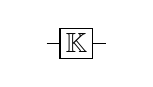
\begin{tikzpicture}[baseline={([yshift=-.5ex]current bounding box.center)}]
    \path (0,0) node (A) {}
    ++ (0.5,0) node[kernel] (K) {$\kernel{K}$}
    ++ (0.5,0) node (B) {};
    \draw (A) -- (K) -- (B);
\end{tikzpicture}\\
\kernel{P}&:= 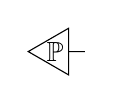
\begin{tikzpicture}[baseline={([yshift=-.5ex]current bounding box.center)}]
    \path (0,0) node[dist] (K) {$\kernel{P}$}
    ++ (0.5,0) node (B) {};
    \draw (K) -- (B);
\end{tikzpicture}
\end{align}

Two Markov kernels $\kernel{L}:X\kto Y$ and $\kernel{M}:Y\kto Z$ have a product $\kernel{L}\kernel{M}:X\kto Z$, given in the discrete case by the matrix product $ \kernel{L}\kernel{M}(z|x) = \sum_{y\in Y} \kernel{M}(z|y)\kernel{L}(y|x)$. Graphically, we represent products between compatible Markov kernels by joining wires together:

\begin{align}
    \kernel{L}\kernel{M}:= 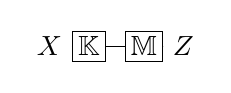
\begin{tikzpicture}[baseline={([yshift=-.5ex]current bounding box.center)}]
    \path (0,0) node (A) {$X$}
    ++ (0.5,0) node[kernel] (K) {$\kernel{K}$}
    ++ (0.7,0) node[kernel] (M) {$\kernel{M}$}
    ++ (0.5,0) node (B) {$Z$};
    \draw (A) -- (K) -- (M) -- (B);
\end{tikzpicture}
\end{align}

The Cartesian product $X\times Y:=\{(x,y)|x\in X, y\in Y\}$. Given kernels $\kernel{K}:W\kto Y$ and $\kernel{L}:X\kto Z$, the tensor product $\kernel{K}\otimes\kernel{L}:W\times X\kto Y\times Z$ given by $(\kernel{K}\otimes\kernel{L})(y,z|w,x):=K(y|w) L(z|x)$. The tensor product is graphically represeted by drawing kernels in parallel:

\begin{align}
    \kernel{K}\otimes \kernel{L}&:=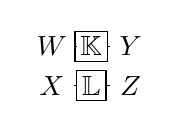
\begin{tikzpicture}[baseline={([yshift=-.5ex]current bounding box.center)}]
    \path (0,0) node (A) {$W$}
    ++ (0.5,0) node[kernel] (K) {$\kernel{K}$}
    ++ (0.5,0) node (B) {$Y$};
    \path (0,-0.5) node (C) {$X$}
    ++ (0.5,0) node[kernel] (L) {$\kernel{L}$}
    ++ (0.5,0) node (D) {$Z$};
    \draw (A) -- (K) -- (B);
    \draw (C) -- (L) -- (D);
\end{tikzpicture}
\end{align}

We read diagrams from left to right (this is somewhat different to \citet{fritz_synthetic_2020,cho_disintegration_2019,fong_causal_2013} but in line with \citet{selinger_survey_2011}), and any diagram describes a set of nested products and tensor products of Markov kernels. There are a collection of special Markov kernels for which we can replace the generic ``box'' of a Markov kernel with a diagrammatic elements that are visually suggestive of what these kernels accomplish.

The identity map $\text{id}_X:X\kto X$ defined by $(\text{id}_X)(x'|x)= \llbracket x = x' \rrbracket$, where the Iverson bracket $\llbracket \cdot \rrbracket$ evaluates to $1$ if $\cdot$ is true and $0$ otherwise, is a bare line:

\begin{align}
    \mathrm{id}_X&:=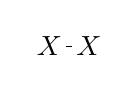
\begin{tikzpicture}[baseline={([yshift=-.5ex]current bounding box.center)}]
    \path (0,0) node (A) {$X$} ++ (0.5,0) node (B) {$X$};
    \draw (A) -- (B);
\end{tikzpicture}
\end{align}

We choose a particular 1-element set $\{*\}$ that acts as the identity in the sense that $\{*\}\times A\cong A\times \{*\} \cong A$ for any set $A$. The erase map $\text{del}_X:X\kto \{*\}$ defined by $(\text{del}_X)(*|x) = 1$ is a Markov kernel that ``discards the input''. It is drawn as a fuse:

\begin{align}
    \text{del}_X&:=\begin{tikzpicture}[baseline={([yshift=-.5ex]current bounding box.center)}]
    \path (0,0) ++ (1,0) node (B) {$X$};
    \draw[-{Rays[n=8]}] (A) -- (B);
\end{tikzpicture}
\end{align}

The copy map $\text{copy}_X:X\kto X\times X$ defined by $(\text{copy}_X)(x',x''|x)=\llbracket x=x' \rrbracket \llbracket x=x'' \rrbracket$ is a Markov kernel that makes two identical copies of the input. It is drawn as a fork:

\begin{align}
    \text{copy}_X&:=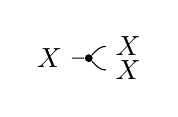
\begin{tikzpicture}[baseline={([yshift=-.5ex]current bounding box.center)}]
    \path (0,0) node (A) {$X$} 
    ++ (0.5,0) node[copymap] (copy0) {}
    ++ (0.5,0.15) node (B) {$X$}
    + (0,-0.3) node (C) {$X$};
    \draw (A) -- (copy0) to [out=45,in=180] (B) (copy0) to [out=-45, in=180] (C);
\end{tikzpicture}
\end{align}

The swap map $\text{swap}_{X,Y}:X\times Y\kto Y\times X$ defined by $(\text{swap}_{X,Y})(y',x'|x,y)=\llbracket x=x' \rrbracket\llbracket y=y' \rrbracket$ swaps two inputs, and is represented by crossing wires:

\begin{align}
    \text{swap}_X &:=  
\begin{tikzpicture}[baseline={([yshift=-.5ex]current bounding box.center)}]
        \path (0,0) node (A) {} 
        + (0,-0.5) node (B) {}
        ++ (1,0) node (C) {}
        + (0,-0.5) node (D) {};
        \draw (A) to [out=0,in=180] (D) (B) to [out=0, in=180] (C);
    \end{tikzpicture}
\end{align}

Because we anticipate that the graphical notation will be unfamiliar, we will include some examples in the next section.

\subsubsection{Examples}

When translating string diagram notation to integral notation, a number of identities can speed up the process.

For arbitrary $\kernel{K}:X\times Y\to Z$, $\kernel{L}:W\to Y$

\begin{align}
 [(\text{id}_X\otimes \kernel{L})\kernel{K}](A|x,w) &= \int_{Y}\int_X   \kernel{K}(z|x',y')\kernel{L}(dy'|w)\text{id}_X(dx'|x)\\
                                           &= \int_Y  \kernel{K}(z|x,y') \kernel{L}(dy'|w)
\end{align}

That is, an identity map passes its input to the next kernel in the product. 

For arbitrary $\kernel{K}: X\times Y\times Y\to Z$ (where we apply the above shorthand in the first line):

\begin{align}
 [(\text{id}_X\otimes \text{copy}_Y)\kernel{K}](A|x,y) &= \int_Y\int_Y \kernel{K}(A|x,y',y'') \text{copy}_Y(dy'\times dy''|y)\\
                                           &= \kernel{K}(A|x,y,y)
\end{align}

That is, the copy map passes along two copies of its input to the next kernel in the product. 

For a collection of kernels $\kernel{K}^n:Y^n\to Z$, $n\in[n]$, define $(y)^{n}=(y|i\in[n])$ and:

\begin{align}
    \text{copy}^n_Y &:= \begin{cases}
    \text{copy}^{n-1}_Y(\text{id}_{Y^{n-2}}\otimes \text{copy}_Y) & n>2\\
    \text{copy}_Y & n=2
    \end{cases}\\
    (\text{copy}^2_Y\kernel{K}^2)(z|y) &= \kernel{K}^2(z|y,y)\\
\end{align}

Suppose for induction
\begin{align}
(\text{copy}^{n-1}_Y\kernel{K}^{n-1})(z|y) &= \kernel{K}^{n-1}(z|(y)^{n-1})
\end{align}

then
\begin{align}
(\text{copy}^n_Y\kernel{K}^n)(z|y) &= (\text{copy}^{n-1}_Y(\text{id}_{Y^{n-2}}\otimes \text{copy}_Y)\kernel{K}^n)(z|y)\\
                                     &= \sum_{y'\in Y^{n-1}}(\text{id}_{Y^{n-2}}\otimes \text{copy}_Y)(\mathbf{y}'|(y)^{n-1})\kernel{K}^n(z|\mathbf{y}')\\
                                     &= \kernel{K}^n(z|(y)^n)
\end{align}

That is, we can define the $n$-fold copy map that passes along $n$ copies of its input to the next kernel in the product.

\subsubsection{Example: comb insertion}

The following examples illustrate 2-combs and the insertion operation, both of which we will define later. As an example in translating diagrams, we show how the diagrams for a 2-comb and 2-comb with an inserted Markov kernel can be translated to integral notation.

Consider the Markov kernels $\kernel{K}:W\kto X$, $\kernel{L}:X\times W\times Y\kto Z$ and the 2-comb $\kernel{M}:W\times Y\kto X\times Z$ defined as

\begin{align}
    \kernel{M} = \tikzfig{2_comb}\label{eq:2comb_M}
\end{align}

Following the rules above, we can translate this to ordinary notation by first breaking it down into products and tensor products, and then evaluating these products

\begin{align}
    \kernel{M}(A\times B|w,y) = [&(\text{copy}_W\otimes \text{id}_Y)(\kernel{K}\otimes \text{id}_{W\times Y})\\
    &(\text{copy}_X\otimes \text{id}_{W\times Y})(\text{id}_X\otimes\kernel{L})](A\times B|w,y)\\
                        = [&(\kernel{K}\otimes \text{id}_{W\times Y})(\text{copy}_X\otimes \text{id}_{W\times Y})\\
                        &(\text{id}_X\otimes\kernel{L})](A\times B|w,w,y)\\
                        = \;&\int_{X}  (\text{id}_X\otimes\kernel{L})(A\times B|x',w,y) \kernel{K} (dx'|w)
                        ](y,z|y',x)\\
                        = \;&\int_X \text{id}_X(A|x') \kernel{L}(B|x',w,y)\kernel{K}(dx'|w)\\
                        = \;&\int_A \kernel{L}(B|x',w,y)\kernel{K}(dx'|w)
\end{align}

If we are given additionally $\kernel{J}:X\times W\kto Y$, we can define a new Markov kernel $\kernel{N}:W\kto Z$ given by ``inserting'' $\kernel{J}$ into $\kernel{M}$:

\begin{align}
    \kernel{N} = \tikzfig{2comb_inserted_anon}\label{eq:2comb_winsert}
\end{align}


We can translate Equation \ref{eq:2comb_winsert} to

\begin{align}
    \kernel{N}(A\times B\times C|w) = &[\text{copy}_W(\kernel{K}\text{copy}^3_Y\otimes \text{id}_W)\\
    &(\text{id}_Y\otimes\kernel{J}\otimes \text{id}_Y)(\text{id}_Y \otimes \text{copy}_X\otimes \text{id}_Y)\\
    &(\kernel{L}\otimes \text{id}_X\otimes \text{id}_Y)] (A\times B\times C|w)\\
                    = &[(\kernel{K}\text{copy}^3_Y\otimes \text{id}_W)(\text{id}_Y\otimes\kernel{J}\otimes \text{id}_Y)\\
                    &(\text{id}_Y \otimes \text{copy}_X\otimes \text{id}_Y)\\
                    &(\kernel{L}\otimes \text{id}_X\otimes \text{id}_Y)] (A\times B\times C|w,w)\\
                    = &\int_X\int_Y\kernel{L}(C|x',w,y') \text{id}_X(A|x') \text{id}_Y(B|y') \kernel{J}(dy'|x',w)\kernel{K}(dx'|w)\\
                    = &\int_A\int_B\kernel{L}(C|x',w,y') \kernel{J}(dy'|x',w)\kernel{K}(dx'|w)
\end{align}

%!TEX root = main.tex


\subsection{Probability sets}\label{sec:probability_sets}

A probability set is a set of probability measures. This section establishes a number of useful properties of conditional probability with respect to probability sets. Unlike conditional probability with respect to a probability space, conditional probabilities don't always exist for probability sets. Where they do, however, they are almost surely unique and we can marginalise and disintegrate them to obtain other conditional probabilities with respect to the same probability set.

\begin{definition}[Probability set]
A probability set $\prob{P}_C$ on $(\Omega,\sigalg{F})$ is a collection of probability measures on $(\Omega,\sigalg{F})$. In other words it is a subset of $\mathscr{P}(\Delta(\Omega))$, where $\mathscr{P}$ indicates the power set.
\end{definition}

Given a probability set $\prob{P}_C$, we define marginal and conditional probabilities as probability measures and Markov kernels that satisfy Definitions \ref{def:pushforward} and \ref{def:disint} respectively for \emph{all} base measures in $\prob{P}_C$. There are generally multiple Markov kernels that satisfy the properties of a conditional probability with respect to a probability set, and this definition ensures that marginal and conditional probabilities are ``almost surely'' unique (Definition \ref{def:asequal}) with respect to probability sets.

\begin{definition}[Marginal probability with respect to a probability set]
Given a sample space $(\Omega,\sigalg{F})$, a variable $\RV{X}:\Omega\to X$ and a probability set $\prob{P}_C$, the marginal distribution $\prob{P}_C^{\RV{X}}=\prob{P}_\alpha^{\RV{X}}$ for any $\prob{P}_\alpha\in\prob{P}_C$ if a distribution satisfying this condition exists. Otherwise, it is undefined.
\end{definition}

\begin{definition}[Uniform conditional distribution]\label{def:cprob_pset}
Given a sample space $(\Omega,\sigalg{F})$, variables $\RV{X}:\Omega\to X$ and $\RV{Y}:\Omega\to Y$ and a probability set $\prob{P}_C$, a uniform conditional distribution $\prob{P}_C^{\RV{Y}|\RV{X}}$ is any Markov kernel $X\kto Y$ such that $\prob{P}_C^{\RV{Y}|\RV{X}}$ is an $\RV{Y}|\RV{X}$ conditional probability of $\prob{P}_\alpha$ for all $\prob{P}_\alpha\in \prob{P}_C$. If no such Markov kernel exists, $\prob{P}_C^{\RV{Y}|\RV{X}}$ is undefined.
\end{definition}

Given a conditional distribution $\mu^{\RV{ZY}|\RV{X}}$ we can define a higher order conditional $\mu^{\RV{Z}|(\RV{Y}|\RV{X})}$, which is a version of $\mu^{\RV{Z}|\RV{XY}}$. This is useful because uniform conditionals don't always exist, but we can use higher order conditionals to show that if a probability set $\prob{P}_C$ has a uniform conditional $\prob{P}_C^{\RV{ZY}|\RV{X}}$ then it also has a uniform conditional $\prob{P}_C^{\RV{Z}|\RV{XY}}$ (Theorems \ref{th:ho_cond_psets} and \ref{th:higher_order_conditionals}). Given $\mu^{\RV{XY}|\RV{Z}}$ and $\RV{X}:\Omega\to X$, $\RV{Y}:\Omega\to Y$ standard measurable, it has recently been proven that a higher order conditional $\mu^{\RV{Z}|(\RV{Y}|\RV{X})}$ exists \citet{bogachev_kantorovich_2020}, Theorem 3.5.

\begin{definition}[Higher order conditionals]
Given a probability space $(\mu,\Omega,\sigalg{F})$ and variables $\RV{X}:\Omega\to X$, $\RV{Y}:\Omega\to Y$ and $\RV{Z}:\Omega\to Z$, a higher order conditional $\mu^{\RV{Z}|(\RV{Y}|\RV{X})}:X\times Y\to Z$ is any Markov kernel such that, for some $\mu^{\RV{Y}|\RV{X}}$, 
\begin{align}
    \mu^{\RV{ZY}|\RV{X}}(B\times C|x) &=\int_B \mu^{\RV{Z}|(\RV{Y}|\RV{X})}(C|x,y)\mu^{\RV{Y}|\RV{X}}(dy|x)\\ 
    &\iff\\
    \mu^{\RV{ZY}|\RV{X}} &= \tikzfig{disintegration_existence}\label{eq:disint_def}
\end{align}
\end{definition}

\begin{definition}[Uniform higher order conditional]\label{def:ho_cprob_pset}
Given a sample space $(\Omega,\sigalg{F})$, variables $\RV{X}:\Omega\to X$, $\RV{Y}:\Omega\to Y$ and $\RV{Z}:\Omega\to Z$ and a probability set $\prob{P}_C$, if $\prob{P}_C^{\RV{ZY}|\RV{X}}$ exists then a uniform higher order conditional $\prob{P}_C^{\RV{Z}|(\RV{Y}|\RV{X})}$ is any Markov kernel $X\times Y\kto Z$ that is a higher order conditional of some version of $\prob{P}_C^{\RV{ZY}|\RV{X}}$. If no $\prob{P}_C^{\RV{ZY}|\RV{X}}$ exists, $\prob{P}_C^{\RV{Z}|(\RV{Y}|\RV{X})}$ is undefined.
\end{definition}


% \begin{lemma}[Equivalence of pushforward definitions]\label{lem:prod_pushf}
% Given a probability space $\kernel{M}:W\to \Omega$ and $\RV{X}:\Omega\to X$, define $\kernel{K}^{\RV{X}|\RV{W}}:W\kto X$ by $\kernel{K}^{\RV{X}|\RV{W}}(x|w):=\kernel{M}(\RV{X}\yields x|w)$ for any $x\in X$m $w\in W$ and $\kernel{L}^{\RV{X}}:W\kto X$ by
% \begin{align}
%   \kernel{L}^{\RV{X}|\RV{W}} = \kernel{M}\kernel{F}_{\RV{X}}
% \end{align}
% Then
% \begin{align}
% \kernel{L}^{\RV{X}|\RV{W}} =\kernel{K}^{\RV{X}|\RV{W}}
% \end{align}
% \end{lemma}

% \begin{proof}
% For any $x\in X$, $w\in W$
% \begin{align}
%   \kernel{L}^{\RV{X}|\RV{W}}(x|w) &= \sum_{\omega\in \Omega} \llbracket x=\RV{X}(\omega)\rrbracket \kernel{M}(\omega|w)\\
%                                   &= \sum_{\omega\in \RV{X}^{-1}(x)} \kernel{M}(\omega|w)\\
%                                   &= \kernel{M}(\RV{X}\yields x|w)\\
%                                   &= \kernel{K}^{\RV{X}|\RV{W}}(x|w)
% \end{align}
% \end{proof}

\begin{definition}[Almost sure equality]
Two Markov kernels $\kernel{K}:X\kto Y$ and $\kernel{L}:X\kto Y$ are $\prob{P}_C,\RV{X},\RV{Y}$-almost surely equal if for all $A\in\sigalg{X}$, $B\in \sigalg{Y}$, $\alpha\in C$
\begin{align}
    \int_A \kernel{K}(B|x)\prob{P}_\alpha^{\RV{X}}(\mathrm{d}x) = \int_A\kernel{L}(B|x)\prob{P}_\alpha^{\RV{X}}(\mathrm{d}x)
\end{align}
we write this as $\kernel{K}\overset{\prob{P}_C}{\cong}\kernel{L}$, as the variables $\RV{X}$ and $\RV{Y}$ are clear from the context.
\end{definition}

Equivalently, $\kernel{K}$ and $\kernel{L}$ are almost surely equal if the set $C:\{x|\exists B\in\sigalg{Y}:\kernel{K}(B|x)\neq\kernel{L}(B|x)\}$ has measure 0 with respect to $\prob{P}_\alpha^{\RV{X}}$ for all $\alpha\in C$.

\subsection{Extended conditional independence}

Just like we defined uniform conditional probability as a version of ``conditional probability'' appropriate for probability sets, we need some version of ``conditional independence'' for probability sets. One such has already been given in some detail: it is the idea of \emph{extended conditional independence} defined in \citet{constantinou_extended_2017}.

We will first define regular conditional independence. We define it in terms of a having a conditional that ``ignores one of its inputs'', which, provided conditional probabilities exists, is equivalent to other common definitions (Theorem \ref{th:cho_ci_equiv}).

\begin{definition}[Conditional independence]\label{def:ci}
For a \emph{probability model} $\model{P}_{\alpha}$ and variables $\RV{A},\RV{B},\RV{Z}$, we say $\RV{B}$ is conditionally independent of $\RV{A}$ given $\RV{C}$, written $\RV{B}\CI_{\model{P}_{\alpha}}\RV{A}|\RV{C}$, if
\begin{align}
    \prob{P}^{\RV{Y}|\RV{WX}} &\overset{\prob{P}}{\cong} \tikzfig{cond_indep_erase}\\
    \iff
    \prob{P}^{\RV{Y}|\RV{WX}}(A|w,x) &\overset{\prob{P}}{\cong} \prob{K}(A|w)&\forall A\in \sigalg{Y}
\end{align}
\end{definition}

Conditional independence can equivalently be stated in terms of the existence of a conditional probability that ``ignores'' one of its inputs.

\begin{theorem}\label{th:cho_ci_equiv}
Given standard measurable $(\Omega,\sigalg{F})$, a probability model $\prob{P}$ and variables $\RV{W}:\Omega\to W$, $\RV{X}:\Omega\to X$, $\RV{Y}:\Omega\to Y$, $\RV{Y}\CI_{\prob{P}}\RV{X}|\RV{W}$ if and only if there exists some version of $\prob{P}^{\RV{Y}|\RV{WX}}$ and $\kernel{K}:W\kto Y$ such that
\begin{align}
    \prob{P}^{\RV{Y}|\RV{WX}} &\overset{\prob{P}}{\cong} \tikzfig{cond_indep_erase}\\
    \iff
    \prob{P}^{\RV{Y}|\RV{WX}}(A|w,x) &\overset{\prob{P}}{\cong} \prob{K}(A|w)&\forall A\in \sigalg{Y}
\end{align}
\end{theorem}

\begin{proof}
See \citet{cho_disintegration_2019}.
\end{proof}

Extended conditional independence as introduced by \citet{constantinou_extended_2017} is defined using ``nonstochastic variables'' on the choice set C. We don't make use of this feature here, and we limit ourselves to a special case of extended conditional independence. 

\begin{definition}[Uniform conditional independence]\label{def:eci}
Given a probability set $\prob{P}_C$ and variables $\RV{X}$, $\RV{Y}$ and $\RV{Z}$, the uniform conditional independence $\RV{Y}\CI^e_{\prob{P}_C} \RV{X} C|\RV{Z}$ holds if $\prob{P}_C^{\RV{Y}|\RV{XZ}}$ and $\prob{P}_C^{\RV{Y}|\RV{X}}$ exist and
\begin{align}
    \prob{P}_C^{\RV{Y}|\RV{XZ}} &\overset{\prob{P}_C}{\cong} \tikzfig{eci_def}\\
    &\iff\\
    \prob{P}_C^{\RV{Y}|\RV{XZ}}(A|x,z) &\overset{\prob{P}_C}{\cong} \prob{P}_C^{\RV{Y}|\RV{Z}}(A|z)&\forall A\in \sigalg{Y},(x,z)\in X\times Z\label{eq:eci}
\end{align}
\end{definition}

Unlike the general definition of extended conditional independence, uniform conditional independence requires that the functions on the right hand side of Equation \ref{eq:eci} are Markov kernels (Definition \ref{def:mkern}). Otherwise, $\RV{Y}\CI^e_{\prob{P}_C} \RV{X} C|\RV{Z}$ is equivalent to the definition provided by \citet{constantinou_extended_2017}, given an appropriate choice of nonstochastic variables.

% Global conditional independence is a weaker condition: we require conditional independence for each $\alpha\in C$, but not the existence of the corresponding uniform conditionals.

% \begin{definition}[Global conditional independence]
% Given a probability set $\prob{P}_C$ and variables $\RV{X}$, $\RV{Y}$ and $\RV{Z}$, the global conditional independence $\RV{Y}\CI^e_{\prob{P}_C} \RV{X} |(\RV{Z},C)$ holds if for all $\alpha\in C$ $\RV{Y}\CI_{\prob{P}_\alpha} \RV{X}|\RV{Z}$.
% \end{definition}

Extended conditional independence requires nonstochastic variables (here, the set ``$C$'') to appear on the right hand side of the $\CI^e$ symbol. Otherwise, for countable sets $C$, we can reason with collections of extended conditional independence statements as if they were regular conditional independence statements. In particular, the following rules hold:

\begin{enumerate}
    \item Symmetry: $\RV{X}\CI_{\prob{P}_C}^e \RV{Y} C|\RV{Z}$ iff $\RV{Y}\CI_{\prob{P}_C}^e \RV{X} C|\RV{Z}$
    \item Decomposition: $\RV{X}\CI_{\prob{P}_C}^e (\RV{Y},\RV{Z})C|\RV{W}$ implies $\RV{X}\CI_{\prob{P}_C}^e\RV{Y}C|\RV{W}$ and $\RV{X}\CI_{\prob{P}}\RV{Z}C|\RV{W}$
    \item Weak union: $\RV{X}\CI_{\prob{P}_C}^e(\RV{Y},\RV{Z})C|\RV{W}$ implies $\RV{X}\CI_{\prob{P}_C}^e\RV{Y}C|(\RV{Z},\RV{W})$
    \item Contraction: $\RV{X}\CI_{\prob{P}_C}^e\RV{Z}C|\RV{W}$ and $\RV{X}\CI_{\prob{P}_C}^e\RV{Y}C|(\RV{Z},\RV{W})$ implies $\RV{X}\CI_{\prob{P}_C}^e(\RV{Y},\RV{Z})C|\RV{W}$
\end{enumerate} 

\subsection{Examples}

\begin{example}[Choice variable]\label{ex:choice_var}
Suppose we have a decision procedure $\proc{S}_C:=\{\proc{S}_\alpha|\alpha\in C\}$ that consists of a measurement procedure for each element of a denumerable set of choices $C$. Each measurement procedure $\proc{S}_\alpha$ is modeled by a probability distribution $\prob{P}_\alpha$ on a shared sample space $(\Omega,\sigalg{F})$ such that we have an observable ``choice'' variable $(\RV{D},\RV{D}\circ\proc{S}_\alpha)$ where $\RV{D}\circ\proc{S}_\alpha$ always yields $\alpha$.

Furthermore, Define $\RV{Y}:\Omega\to \Omega$ as the identity function. Then, by supposition, for each $\alpha\in A$, $\prob{P}_\alpha^{\RV{Y}\RV{C}}$ exists and for $A\in \sigalg{Y}$, $B\in \sigalg{C}$:

\begin{align}
    \prob{P}_\alpha^{\RV{YC}}(A\times B) &= \prob{P}_\alpha(A)\delta_\alpha(B)
\end{align}

This implies, for all $\alpha\in C$

\begin{align}
    \prob{P}_\alpha^{\RV{Y}|\RV{D}} &= \prob{P}_\alpha^{\RV{Y}}
\end{align}

Thus $\prob{P}_C^{\RV{Y}|\RV{D}}$ exists and

\begin{align}
    \prob{P}_C^{\RV{Y}|\RV{D}}(A|\alpha) &= \prob{P}_\alpha^{\RV{Y}} (A)&\forall A\in \sigalg{Y},\alpha\in C 
\end{align}

Because only deterministic marginals $\prob{P}_\alpha^{\RV{D}}$ are available, for every $\alpha\in C$ we have $\RV{Y}\CI_{\prob{P}_\alpha} \RV{D}$. This reflects the fact that \emph{after we have selected a choice $\alpha$} the value of $\RV{C}$ provides no further information about the distribution of $\RV{Y}$, because $\RV{D}$ is deterministic given any $\alpha$. It does not reflect the fact that ``choosing different values of $\RV{C}$ has no effect on $\RV{Y}$''.
\end{example}

\begin{theorem}[Uniform conditional independence representation]\label{th:uci_rep}
Given a probability set $\prob{P}_C$ with a uniform conditional probability $\prob{P}^{\RV{XY}|\RV{Z}}_C$,
\begin{align}
    \prob{P}^{\RV{XY}|\RV{Z}}_C &\overset{\prob{P}_C}{\cong} \tikzfig{eci_rep}\\
    &\iff\\
    \prob{P}^{\RV{XY}|\RV{Z}}_C(A\times B|z) &\overset{\prob{P}_C}{\cong} \prob{P}_C^{\RV{X}|\RV{Z}}(A|z)\prob{P}_C^{\RV{Y}|\RV{Z}}(B|z)&\forall A\in \sigalg{X},B\in \sigalg{Y},z\in Z
\end{align}
if and only if $\RV{Y}\CI_{\prob{P}_C}^e \RV{X}C|\RV{Z}$
\end{theorem}

\begin{proof}
If:
By Theorem \ref{th:higher_order_conditionals}
\begin{align}
    \prob{P}^{\RV{XY}|\RV{Z}}_C &= \tikzfig{eci_rep_1}\\
    &\overset{\prob{P}_C}{\cong} \tikzfig{eci_rep_2}\\
    &= \tikzfig{eci_rep}
\end{align}
Only if:
Suppose
\begin{align}
    \prob{P}^{\RV{XY}|\RV{Z}}_C &\overset{\prob{P}_C}{\cong} \tikzfig{eci_rep}
\end{align}
and suppose for some $\alpha\in C$, $A\times C\in \sigalg{X}\otimes\sigalg{Z}$, $B\in \sigalg{Y}$ $\prob{P}_\alpha^{\RV{XZ}}(A\times C)>0$ and
\begin{align}
    \prob{P}_C^{\RV{Y}|\RV{XZ}}(B|x,z) &> \prob{P}_C^{\RV{Y}|\RV{Z}}(B|z)& \forall (x,z)\in A\times C \label{eq:assume_ieq}
\end{align}
then
\begin{align}
    \prob{P}_\alpha^{\RV{XYZ}\RV{Z}}(A\times B\times C) &= \int_{A\times C} \prob{P}_C^{\RV{Y}|\RV{XZ}}(B|x,z)\prob{P}_C^{\RV{X}|\RV{Z}}(\mathrm{dx}|z)\prob{P}_\alpha^{\RV{Z}}(\mathrm{dz})\\
    &> \int_{A\times C} \prob{P}_C^{\RV{Y}|\RV{X}}(B|z)\prob{P}_C^{\RV{X}|\RV{Z}}(\mathrm{dx}|z)\prob{P}_\alpha^{\RV{Z}}(\mathrm{dz})\\
    &= \int_{C} \prob{P}_C^{\RV{XY}|\RV{X}}(A\times B|z)\prob{P}_\alpha^{\RV{Z}}(\mathrm{dz})\\
    &= \prob{P}_\alpha^{\RV{XYZ}\RV{Z}}(A\times B\times C)
\end{align}
a contradiction. An analogous argument follows if we replace ``$>$'' with ``$<$'' in Eq. \ref{eq:assume_ieq}.
\end{proof}

% \begin{theorem}[Disintegrations are conditional probabilities]
% Suppose we have a fundamental probability set $\Omega$ variables $\RV{W}:\Omega\to W$, $\RV{X}:\Omega\to X$, $\RV{Y}:\Omega\to Y$ and $\RV{Z}:\Omega\to Z$ and a probability set $\prob{P}_C$ such that $\prob{P}_C^{\RV{X}|\RV{Y}}$ is a $\RV{Y}|\RV{X}$ conditional probability and there is some $\kernel{K}^{\RV{$
% \end{theorem}

% Given a conditional probability with respect to a probability gap model, we can also find additional conditional probabilities by disintegrating the original conditional probability.

% \begin{lemma}[Recursive disintegration]
% Suppose we have a fundamental probability set $\Omega$, variables $\RV{W}:\Omega\to W$, $\RV{X}:\Omega\to X$ and $\RV{Y}:\Omega\to Y$, $\RV{Z}:\Omega\to Z$ and a probability set $\prob{P}_C$ such that $\prob{P}_C^{\RV{X}|\RV{Y}}$ is a $\RV{Y}|\RV{X}$ conditional probability. Define $\prob{Q}_C$ as the largest probability set such that $\prob{Q}_C^{\RV{Y}|\RV{X}}=\prob{P}_C^{\RV{Y}|\RV{X}}$. Then if $\prob{Q}_C^{\RV{Z}|\RV{W}}$ is a $\RV{Z}|\RV{W}$ conditional probability of $\prob{Q}_C$, it is also a $\RV{Z}|\RV{W}$ conditional probability of $\prob{P}_C$.
% \end{lemma}

% \begin{proof}
% $\prob{Q}_C\supset \prob{P}_C$, so any conditional probability of $\prob{Q}_C$ is also a conditional probability of $\prob{P}_C$.
% \end{proof}



% \begin{definition}[Conditional independence with respect to a probability comb]
% Conditional independence $\RV{A}\CI_{\prob{P}_\square}\RV{B}|\RV{C}$ holds for an arbitrary probability comb $\model{P}_\square:A\to \mathscr{P}(\Delta(\Omega))$ if $\RV{A}\CI_{\prob{P}_\alpha}\RV{B}|\RV{C}$ holds for all probability models $\prob{P}_\alpha$, $\alpha\in A$.
% \end{definition}

%!TEX root = main.tex



\section{Syntax and semantics of causal consequences}

Causal Bayesian networks and potential outcomes employ different naming conventions to distinguish ``causal effects'' from ``simple correlations''. Causal Bayesian networks write $P(\RV{Y}|do(\RV{X}))$ and $P(\RV{Y}|\RV{X})$, while potential outcomes distinguishes $P(\RV{Y}|\RV{X})$ from $x\mapsto P(\RV{Y}^x)$. If we are not going to worry too much about details of interpretation, we can interpret the expression $P(\RV{Y}|\RV{X})$ as expressing something like this: there is an objective probability $P(\RV{Y},\RV{X})$ that describes a sequence of independent and identically distributed observations, and $P(\RV{Y}|\RV{X})$ is a disintegration of this probability. The existence of an objective probability $P(\RV{Y},\RV{X})$ can be justified by an assumption that the sequence of observations should be modeled exchangeably.

We pursue a similar line of thinking with respect to understanding causal consequences like $P(\RV{Y}|do(\RV{X}))$ or $x\mapsto P(\RV{Y}^x)$. We assume that ``causal consequences'' are conditional probabilities of the form $\prob{P}_\square^{\RV{Y}|\RV{D}\RV{H}}$ where $\RV{Y}$ is an outcome, $\RV{D}$ is some decision, $\RV{H}$ is a hypothesis and $\prob{P}_\square$ is a probability gap model. Our interest is in understanding what causal consequences are \emph{from the point of view of someone choosing a decision function}. We do not address the question of how they may be inferred from observed data.

 We show that conditional probability models that are \emph{causally contractible} with respect to a sequence of decisions and a corresponding sequence of outcomes are representible by mixtures of ``objective but unknown'' conditional probabilities. This is analogous to De Finetti's theorem that shows exchangeable probability distributions are representable by mixtures of ``objective but unknown'' independent and identically distributed probability distributions. A similar argument to ours is found in \citet{dawid_decision-theoretic_2020}.

We also consider the question of when causal contractibility could be supposed to hold. This is a subtle question, as the answer appears to differ for situations that are quite similar. For example, consider:
\begin{enumerate}
    \item Dr Alice is going to see two patients who are both complaining of lower back pain and are otherwise unknown to Alice. Prior to seeing them, she considers the available research and formulates a general sense of whether or not she'll treat each one, which she quantifies with $\prob{P}_\alpha^{\RV{D}_1\RV{D}_2}$
    \item As before, but prior to seeing the patients she considers the available research and decides to treat on the basis of applying a function to a random number generator with known characteristics. The choice of function and random number generator allow her to quantity probability of treatment with $\prob{P}_\alpha^{\RV{D}_1\RV{D}_2}$
\end{enumerate}

\todo[inline]{I removed the discussion of probability combs for simplicity, so I have not considered policies for treatment that depend on earlier experiments in the examples above}

We will argue that Alice could reasonably assume causal contractibility in the second case but not the first. While we are unable to offer a general theory of when causal contractibility holds, we note that an apparently key difference between the two situations is that in the first case the ``decision'' $\RV{D}_1$ is indeterministic for some $\alpha$, though $\RV{D}_2$ is deterministic, while in the second case both $\RV{D}_1$ and $\RV{D}_2$ are determinstic functions.

\subsection{Repeatable experiments}

A conditional probability model $(\prob{P}_\square^{\overline{\RV{Y}|\RV{D}}},A)$ is a model of a sequential experiment if $\RV{Y}:=\RV{Y}_M=(\RV{Y}_i)_{i\in M}$ and $\RV{D}:=\RV{D}_M=(\RV{D}_i)_{i\in M}$ for some index set $M$. We say that $\RV{Y}_i$ is the consequence corresponding to the decision $\RV{D}_i$ for all $i\in M$. We identify a ``causal consequence'' with a conditional probability of the form $\prob{P}_\square^{\RV{Y}_i|\RV{H}\RV{D}_i}$, where $\RV{H}$ is a hypothesis that is deterministically identical for every $i$. Causal consequences do not generally exist, see Definition \ref{def:cprob_pset}.

If $(\prob{P}_\square^{\overline{\RV{Y}|\RV{D}}},A)$ represents a sequential experiment, we might guess that causal consequences exist if the experiment is in some sense ``repeatable''. We consider two precise notions of repeatability. The first condition is \emph{commutativity of exchange}, which is the assumption that swapping the choices that we apply at each step and then applying the corresponding inverse swap to consequences leaves the model unchanged. The second condition is \emph{commutativity of marginalisation} -- if we perform the whole experiment multiple times, making the same choice $\RV{D}_i$ at any point $i$ gets the same results, regardless of what other choices are made.

Commutativity of exchange is similar to the condition of \emph{post-treatment exchangeability} found in \citet{dawid_decision-theoretic_2020}, and commutativity of marginalisation is similar to the stable unit treatment distribution assumption (SUTDA) in the same, as well as the ``no interference'' part of the stable unit treatment value assumption (SUTVA) with which it shares a name. Commutativity of exchange is also very similar to the exchangeability assumption of \citet{greenland_identifiability_1986} for further discussions of exchangeability in the context of causal modelling, and note that both authors consider exchanging to be an operation that alters which person receives which treatment. The assumption of exchangeability found in \citet{banerjee_chapter_2017} can also be regarded as similar to commutativity of exchange.

\todo[inline]{Not sure if or where I want to put this, I just think it helps to illustrate the difference}

Commutativity of exchange is not equivalent to exchangeability in the sense of De Finetti's well-known theorem \citet{de_finetti_foresight_1992}. The latter can be understood as expressing an indifference between conducting the experiment as normal, or conducting the experiment and then swapping some labels. However, swapping \emph{choices} will (usually) lead to different ``pieces of the experiment'' receiving different treatment, which is something that can't be achieved by swapping labels after the experiment has concluded.

The difference is illustrated by the following pair of diagrams.

Exchangeability (swapping labels):

\begin{align}
    \tikzfig{exchangeability}
\end{align}

Commutativity of exchange (swapping choices $\sim$ swapping labels):

\begin{align}
    \tikzfig{commutativity of exchange}
\end{align}

Commutativity of exchange is a property of probability gap models, not a property of fixed probability model for which there is no analogue of ``attaching a different choice'' in that case.

\todo[inline]{----end not sure where to put------}


% Another way to see where we are going is to consider graphical statements of our and De Finetti's result.

% Take $S=\{0,1\}$ and identify the space $\Delta(S)$ of probability measures on $S$ with the interval $[0,1]$. De Finetti showed that any infinite exchangeable probability measure $\prob{P}_\alpha$ on $\{0,1\}^\mathbb{N}$ can be represented by a prior $\prob{P}_\alpha^{\RV{H}}\in [0,1]$ for some $\RV{H}:\Omega\to H$ and a conditional probability $\prob{P}^{\RV{S}_0|\RV{H}}:[0,1]\kto \{0,1\}$ such that

% \begin{align}
%     \prob{P}_\alpha &= \tikzfig{de_finetti_rep0}\label{eq:definettirep}
% \end{align}

% Here $\prob{P}^{\RV{S}_0|\RV{H}}$ can be defined concretely by $\prob{P}^{\RV{S}_0|\RV{H}}(1|h)=h$. Equivalently, the probability gap model on $S^\mathbb{N}$ defined by the assumption of exchangeability is equivalent to the probability gap model defined by the conditional probability

% \begin{align}
%     \prob{P}^{\RV{S}|\RV{H}} = \tikzfig{de_finetti_conditional}
% \end{align}

% That is, there is some hypothesis $\RV{H}$ and conditional on $\RV{H}$ the measurements are independent and identically distributed. The proof of this is constructive -- $\RV{H}$ is a function of $\RV{S}$.



% \begin{align}
%     \prob{P}^{\RV{Y}|\RV{HD}} = \tikzfig{do_model_representation}
% \end{align}

% We will further argue that the class of see-do models considered in CBN and potential outcomes literature is equivalent to the family of causally contractible and exchangeable do-models where the decision rule for the first $n$ places is fixed to an unknown value, and may be freely chosen thereafter.

% \begin{theorem}[Existence of conditional in do models]
% Given a do model $(\prob{P}_{\square}^{\RV{Y}\|\RV{D}},R)$, for all $\alpha\in R$, $n\in\mathbb{N}$
% \begin{align}
%     \prob{P}_\alpha^{\RV{Y}_{[n]}\RV{D}_i} = \prob{P}_\alpha^{\RV{D}_{[n]}}\odot \prob{P}_\square^{\RV{Y}_{[n]}\|\RV{D}_{[n]}}
% \end{align}
% That is, $\prob{P}_\square^{\RV{Y}_{[n]}\|\RV{D}_{[n]}}\cong \prob{P}_\square^{\RV{Y}_{[n]}|\RV{D}_{[n]}}$
% \end{theorem}

% \begin{proof}
% For any $n>1\in \mathbb{N}$, $\alpha\in R$

% \begin{align}
%     \prob{P}_\alpha^{\RV{Y}_{[n]}\RV{D}_{[n]}} &= \tikzfig{do_model_1}\\
%     &= \tikzfig{do_model_2}\\
%     &= \tikzfig{do_model_3}\\
%     &= \tikzfig{do_model_4}\\
%     \implies \prob{P}_\alpha^{\RV{Y}_{[n]}|\RV{D}_{[n]}} &= \tikzfig{do_model_5}\\
%     &= \prob{P}_\alpha^{\RV{Y}_{[n-1]}|\RV{D}_{[n-1]}}\combprod \prob{P}_\square^{\RV{Y}_n|\RV{Y}_{[n-1]}\RV{D}_n}
% \end{align}

% Applying this recursively with $\prob{P}_\alpha^{\RV{Y}_{[1]}|\RV{D}_{[1]}}=\prob{P}_\square^{\RV{Y}_{[1]}|\RV{D}_{[1]}}$ yields

% \begin{align}
%     \prob{P}_\alpha^{\RV{Y}_{[n]}|\RV{D}_{[n]}} = \prob{P}_\square^{\RV{Y}_{[n]}\|\RV{D}_{[n]}}
% \end{align}
% as desired.
% \end{proof}
More precisely, a conditional probability model ``commutes with exchange'' if applying any finite permutation to blind choices or separately applying the corresponding permuation to consequences each yields the same result. We can apply the exchange ``before'' multiplying by the conditional $\prob{P}_{\square}^{\RV{Y}|\RV{D}}$ or after it and we get the same result.

\begin{definition}[Swap map]
Given $M\subset \mathbb{N}$ a finite permutation $\rho:M\to M$ and a variable $\RV{X}:\Omega\to X^M$ such that $\RV{X}=(\RV{X}_i)_{i\in M}$, define the Markov kernel $\text{swap}_{\rho(\RV{X})}:X^M\kto X^M$ by $(d_i)_{i\in\mathbb{N}}\mapsto \delta_{(d_{\rho(i)})_{i\in\mathbb{N}}}$.
\end{definition}

\begin{definition}[Commutativity of exchange]\label{def:caus_exch}
Suppose we have a sample space $(\Omega,\sigalg{F})$ and a conditional probability model $(\prob{P}_{\square}^{\overline{\RV{Y}|\RV{D}}},A)$ with $\RV{Y}=\RV{Y}_M$, $\RV{D}=\RV{D}_M$, $M\subseteq \mathbb{N}$. If, for any two decision rules $\alpha^{\overline{\RV{D}}},\beta^{\overline{\RV{D}}} \in A$,
\begin{align}
    \alpha^{\RV{D}}\odot \text{swap}_{\rho(\RV{D})} \prob{P}_{\square}^{\RV{Y}|\RV{D}} &= \alpha^{\RV{D}}\odot \prob{P}_{\square}^{\RV{Y}|\RV{D}}\text{swap}_{\rho(\RV{Y})}
\end{align}
Then $\prob{P}_\square$ \emph{commutes with exchanges}.
\end{definition}

A do model is non interfering if it gives identical results for identical subsequences of different choices when we limit our attention to the corresponding subsequences of consequences. For example, if we have $\RV{D}=(\RV{D}_1,\RV{D}_2,\RV{D}_3)$ and $\RV{Y}=(\RV{Y}_1,\RV{Y}_2,\RV{Y}_3)$ and $\alpha^{\RV{D}_1\RV{D}_3}=\prob{P}_\beta^{\RV{D}_1\RV{D}_3}$ then $\prob{P}_{\alpha}^{\RV{Y}_1\RV{D}_1\RV{Y}_3\RV{D}_3}=\prob{P}_\beta^{\RV{Y}_1\RV{D}_1\RV{Y}_3\RV{D}_3}$.

\begin{definition}[Commutativity of marginalisation]\label{def:caus_cont}
Suppose we have a sample space $(\Omega,\sigalg{F})$ and a conditional probability model $(\prob{P}_{\square}^{\overline{\RV{Y}|\RV{D}}},A)$ with $\RV{Y}=\RV{Y}_M$, $\RV{D}=\RV{D}_M$, $M\subseteq \mathbb{N}$. For any $S=(s_i)_{i\in Q}$, $Q\subset M$, and $i<j\implies p_i<p_j \And q_i<q_j$, let $\RV{D}_S:=(\RV{D}_i)_{i\in S}$ and $\RV{D}_T:=(\RV{D}_i)_{i\in T}$. If for any $\alpha,\beta\in R$
\begin{align}
    \prob{P}_\alpha^{\RV{D}_{S}}&=\prob{P}_\beta^{\RV{D}_{S}}\\
    \implies \prob{P}_\alpha^{(\RV{D_i,Y_i})_{i\in S}}&=\prob{P}_\beta^{(\RV{D_i,Y_i})_{i\in S}}
\end{align}
then $\prob{P}_\square$ \emph{commutes with marginalisation}.
\end{definition}

Neither condition implies the other. 
\begin{lemma}
Commutativity of exchange does not imply commutativity or vise versa.
\end{lemma}

\begin{proof}
Suppose $D=Y=\{0,1\}$ and we have a conditional probability model $(\prob{P}_\square^{\overline{\RV{Y}|\RV{D}}},A)$ where $\RV{D}=(\RV{D}_1,\RV{D}_2)$, $\RV{Y}=(\RV{Y}_1,\RV{Y}_2)$ and A contains all deterministic probability measures in $\Delta(D^2)$. If

\begin{align}
    \prob{P}_\square^{\RV{Y}_1\RV{Y}_2|\RV{D}_1\RV{D}_2}(y_1,y_2|d_1,d_2) &= \llbracket (y_1,y_2)= (d_1+d_2,d_1+d_2) \rrbracket
\end{align}

Then $\prob{P}_{\delta_{00}}^{\RV{Y}_1\RV{D}_1}(y_1) = \llbracket y_1=0\rrbracket$ while $\prob{P}_{\delta_{01}}^{\RV{Y}_1} = \llbracket y_1=1 \rrbracket$. However, $\delta_00^{\RV{D}_1}=\delta_{01}^{\RV{D}_1}=\delta_0^{\RV{D}_1}$ so $\prob{P}_\square$ does not commute with marginalisation. However, taking $(d_i,d_j):=\delta_{d_i d_j}\in A$,

\begin{align}
    \prob{P}_{d_2,d_1}^{\RV{Y}_1\RV{D}_1\RV{Y}_2\RV{D}_2}(y_1,d_1,y_2,d_2) &= \llbracket (y_1,y_2)= (d_2+d_1,d_2+d_1) \rrbracket\\
    &= \llbracket (y_2,y_1)= (d_1+d_2,d_1+d_2) \rrbracket\\
    &= \prob{P}_{d_1,d_2}^{\RV{Y}_1\RV{D}_1\RV{Y}_2\RV{D}_2}(y_2,d_2,y_1,d_1)
\end{align}

so $\prob{P}_\square$ commutes with exchange.

Alternatively, suppose the same setup, but define $\prob{P}_\square$ instead by, for all $\alpha\in A$

\begin{align}
    \prob{P}_\square{\RV{Y}_1\RV{Y}_2|\RV{D}_1\RV{D}_2}(y_1,y_2|d_1,d_2) &= \llbracket (y_1,y_2)= (0,1) \rrbracket
\end{align}

Then $\prob{P}_\square$ commutes with marginalisation. If $\prob{P}_\alpha^{\RV{D}_S}=\prob{P}_\beta^{\RV{D}_S}$ for $S\subset\{0,1\}$ then

\begin{align}
    \prob{P}_{\alpha}^{\RV{Y}_S\RV{D}_S}(y_s,d_s) &= \sum_{y'_2\in \{0,1\}^{S^C}} \llbracket (y_1,y_2)= (0,1) \rrbracket\prob{P}_\alpha^{\RV{D}_S}(d_s) \\
                                                  &= \prob{P}_{\beta}^{\RV{Y}_S\RV{D}_S}(y_s,d_s)
\end{align}
but not exchange. For all $\alpha,\beta \in A$:

\begin{align}
    \prob{P}_\alpha{\RV{Y}_1\RV{Y}_2}(y_1,y_2) &= \llbracket (y_1,y_2)= (0,1) \rrbracket\\
    &\neq \prob{P}_\beta{\RV{Y}_1\RV{Y}_2}(y_2,y_1)
\end{align}
\end{proof}

Although commutativity of marginalisation seems to be a bit like non-interference -- the marginal distribution I get for $\RV{Y}_i$ depends only on the decision $\RV{D}_i$ -- it still allows for some models in which we seem to have interference of a kind. For example: in the first experiment I flip a coin and decide either to pass the results to the second experiment ($\RV{D}_1=0$) or flip another coin and pass those results second experiment ($\RV{D}_1=1$). In the second I either copy the results I have been given ($\RV{D}_2=0$) or invert them ($\RV{D}_2=1$). Then
\begin{itemize}
    \item The marginal distribution of both experiments is $\text{Bernoulli}(0.5)$ no matter what choices I make, so it satisfies Definition \ref{def:caus_cont}
    \item Nevertheless, the choice for the first experiment seems to ``affect'' the result of the second experiment (affect in quotes because it is an intuitive judgement, not a formal property)
\end{itemize}

Here we are most interested in the conjunction of these assumptions, a condition we call \emph{causal contractibility}

\begin{definition}[Causal contractibility]
A conditional probability model $(\prob{P}_{\square}^{\overline{\RV{Y}|\RV{D}}},A)$ is causally contractible if it is both commutative with exchange and commutative with marginalisation.
\end{definition}

% \begin{proposition}[Representation of do-models that commute with exchange]
% Suppose we have a fundamental probability set $\Omega$ and a do model $(\prob{P},\RV{D},\RV{Y},R)$ such that $\RV{D}:=(\RV{D}_i)_{i\in \mathbb{N}}$ and $\RV{Y}:=(\RV{Y}_i)_{i\in\mathbb{N}}$ where $\prob{P}$ commutes with exchange and there is some $\alpha^*\in R$ such that $\prob{P}^{\alpha^*}\gg\prob{P}_\beta$ for all $\beta in R$. Then there exists a symmetric function $\RV{H}:(Y\times D)^\mathbb{N}\to H$ such that  $\prob{P}^{\RV{Y}|\RV{DH}}$ exists and $\RV{Y}_i\CI_{\prob{P}}(\RV{D}_j,\RV{Y}_j)_{j\in \mathbb{N}}\setminus \{i\}|\RV{H}\RV{D}_i$, or equivalently 
% \begin{align}
%     \prob{P}^{\RV{Y}} &= \tikzfig{do_model_representation}
% \end{align}
% \end{proposition}

% % \begin{lemma}[Contraction and independence]
% % Let $\RV{J}$, $\RV{K}$ and $\RV{L}$ be variables on $\Omega$ and $\prob{Q}\in \Delta(\Omega)$ a base measure such that $\prob{Q}^{\RV{JK}}=\prob{Q}^{\RV{JL}}$ and $\sigma{K}\subset \sigma{L}$. Then $\RV{J}\CI\RV{L}|\RV{K}$. 
% % \end{lemma}

% % \begin{proof}
% % From Lemma 1.3 in \citet{kallenberg_basic_2005}.
% % \end{proof}

% \begin{proof}
% If $\prob{P}$ commutes with exchange, then for any $\alpha\in R$ such that $\prob{P}_\alpha^{\RV{D}}$ is exchangeable then $\prob{P}_\alpha$ is also exchangeable. Then there exists $\RV{H}$ a symmetric function of $(\RV{Y}_i,\RV{D}_i)_{i\in\mathbb{N}}$ such that $\RV{Y}_i\CI_{\prob{P}}(\RV{D}_j,\RV{Y}_j)_{j\in \mathbb{N}}\setminus \{i\}|\RV{H}\RV{D}_i$. This is De Finetti's representation theorem, and many proofs exists, see for example \citep{kallenberg_basic_2005}.

% In particular, let 

% \begin{align}
%     \RV{H}:=A\times B\mapsto \lim_{n\to\infty} \frac{1}{n}\sum_{i\in n} \mathds{1}_{A\times B}((\RV{Y}_i, \RV{D}_i))
% \end{align}

% Then for all $\alpha\in R$,
% \begin{align}
%     \prob{P}_\alpha^{(\RV{Y}_i,\RV{D}_i)_{i\in\mathbb{N}}|\RV{H}}(A\times B|h) \overset{a.s.}{=} h(A\times B)\label{eq:given_h}
% \end{align}

% The proof that the limit exists and the above equality holds can again be found int \citep{kallenberg_basic_2005}.
% \end{proof}

\subsection{Causal consequences exist if the model is causally contractible}

The main result in this section is Theorem \ref{th:iid_rep} which shows that a conditional probability model $\prob{P}_\square$ is causally contractible if and only if it can be represented as the product of a distribution over hypotheses $\prob{P}_\square^{\RV{H}}$ and a collection of identical conditional probabilities $\prob{P}_\square^{\RV{Y}_1|\RV{D}_1\RV{H}}$. This can be interpreted as expressing the idea that all $(\RV{Y}_i,\RV{D}_i)$ pairs share a canonical but unknown ``consequence function'' $D\kto Y$. As discussed in Section \ref{sec:curry}, the existence of such a consequence function implies the existence of a common unknown curried consequence function. Curried consequence functions look very similar to potential outcomes models, but they don't necessarily support any counterfactual interpretation.

\begin{lemma}[Exchangeable curried representation]\label{th:table_rep}
A conditional probability model $(\prob{P}^{\RV{Y}|\RV{D}}_\square,A)$ such that $\RV{D}:=(\RV{D}_i)_{i\in \mathbb{N}}$ and $\RV{Y}:=(\RV{Y}_i)_{i\in \mathbb{N}}$. $\prob{P}_\square$ is causally contractible if and only if
\begin{align}
    \prob{P}_\square^{\RV{Y}|\RV{D}} &= \tikzfig{lookup_representation}\\
    &\iff\\
    \prob{P}_\square^{\RV{Y}|\RV{D}}(y|d) &= \prob{P}^{(\RV{Y}^D_{d_i i})_{\mathbb{N}}}(y)
\end{align}
Where $\prob{P}^{\RV{Y}^D}$ is an exchangeable probability measure on $Y^{D\times\mathbb{N}}$, for convenience we extend the sample space with the random variable $\RV{Y}^D:=(\RV{Y}_{ij}^D)_{i\in D,j\in \mathbb{N}}$ and $\prob{L}^{\RV{D},\RV{Y}^D}$ is the Markov kernel associated with the lookup function
\begin{align}
    l:D^\mathbb{N}\times Y^{D\times \mathbb{N}}&\to Y\\
    ((d_i)_\mathbb{N},(y_{ij})_{i\in D,j\in \mathbb{N}})&\mapsto y_{d_i i}
\end{align}
\end{lemma}

\begin{proof}
Only if:
Choose $e:=(e_i)_{i\in\mathbb{N}}$ such that $e_{|D|i+j}$ is the $i$th element of $D$ for all $i,j\in \mathbb{N}$. Abusing notation, write $e$ also for the decision function that chooses $e$ deterministically.

Define
\begin{align}
    \prob{P}^{\RV{Y}^D}((y_{ij})_{D\times \mathbb{N}}):=\prob{P}_e^{\RV{Y}}((y_{|D|i+j})_{i\in D, j\in \mathbb{N}})
\end{align}

Now consider any $d:=(d_i)_{i\in \mathbb{N}}\in D^{\mathbb{N}}$. By definition of $e$, $e_{|D|d_i + i}=d_i$ for any $i,j\in \mathbb{N}$.

\begin{align}
    \prob{Q}:D\kto Y\\
    \prob{Q}:= \tikzfig{lookup_representation}
\end{align}

and consider some ordered sequence $A\subset \mathbb{N}$ and $B:= ((|D|d_i+i))_{i\in A}$. Note that $e_B:=(e_{|D|d_i +i})_{i\in B}=d_A=(d_i)_{i\in A}$. Then 

\begin{align}
    \sum_{y\in \RV{Y}^{-1}(y_A)} \prob{Q}(y|d) &= \sum_{y\in \RV{Y}^{-1}(y_A)} \prob{P}^{(\RV{Y}^{D}_{d_ii})_{A}}(y) \\
    &= \sum_{y\in \RV{Y}^{-1}(y_A)} \prob{P}_e^{(\RV{Y}_{|D|d_i+i})_{A}}(y)\\
    &= \prob{P}_e^{\RV{Y}_{B}}(y_A)\\
    &= \prob{P}_{d}^{\RV{Y}_A}(y_A)&\text{by causal contractibility}
\end{align}

Because this holds for all $A\subset\mathbb{N}$, by the Kolmogorov extension theorem

\begin{align}
    \prob{Q}(y|d) &= \prob{P}_d^{\RV{Y}}(y)
\end{align}

Because $d$ is the decision function that deterministically chooses $d$, for all $d\in D$

\begin{align}
    \prob{Q}(y|d) &= \prob{P}_d^{\RV{Y}|\RV{D}}(y|d)
\end{align}

And because $\prob{P}_d^{\RV{Y}|\RV{D}}(y|d)$ is unique for all $d\in D^{\mathbb{N}}$ and $\prob{P}^{\RV{Y}|\RV{D}}$ exists by assumption

\begin{align}
    \prob{P}^{\RV{Y}|\RV{D}}=\prob{Q}
\end{align}

Next we will show $\prob{P}^{\RV{Y}^D}$ is contractible. Consider any subsequences $\RV{Y}^D_S$ and $\RV{Y}^D_T$ of $\RV{Y}^D$ with $|S|=|T|$. Let $\rho(S)$ be the ``expansion'' of the indices $S$, i.e. $\rho(S)=(|D|i+j)_{i\in S,j\in D}$. Then by construction of $e$, $e_{\rho(S)}=e_{\rho(T)}$ and therefore

\begin{align}
    \prob{P}^{\RV{Y}^D_S}&= \prob{P}_e^{\RV{Y}_{\rho(S)}})\\
    &= \prob{P}_e^{\RV{Y}_{\rho(T)}})&\text{by contractibility of }\prob{P}\text{ and the equality } e_{\rho(S)}=e_{\rho(T)}\\
    &= \prob{P}^{\RV{Y}^D_T}
\end{align}


If:
Suppose 
\begin{align}
    \prob{P}^{\RV{Y}|\RV{D}} &= \tikzfig{lookup_representation}
\end{align}

and consider any two deterministic decision functions $d,d'\in D^{\mathbb{N}}$ such that some subsequences are equal $d_S=d'_T$.

Let $\RV{Y}^{d_S}=(\RV{Y}_{d_i i})_{i\in S}$.

By definition,

\begin{align}
    \prob{P}^{\RV{Y}_S|\RV{D}}(y_S|d) &= \sum_{y^D_S\in Y^{|D|\times |S|}}\prob{P}^{\RV{Y}^D_S}(y^D_S)\prob{L}^{\RV{D}_S,\RV{Y}^S}(y_S|d,y^D_S)\\
    &= \sum_{y^D_S\in Y^{|D|\times |T|}}\prob{P}^{\RV{Y}^D_T}(y^D_S)\prob{L}^{\RV{D}_S,\RV{Y}^S}(y_S|d,y^D_S)&\text{ by contractibility of }\prob{P}^{\RV{Y}^D_T}\\
    &= \prob{P}^{\RV{Y}_T|\RV{D}}(y_S|d)
\end{align}
\end{proof}

The curried representation of Lemma \ref{th:table_rep} does not need to support an interpretation as a distribution of potential outcomes. For example, consider a series of bets on fair coinflips -- in this case, the consequence $\RV{Y}_i$ is uniform on $\{0,1\}$ for any decision $\RV{D}_i$. Tha $D=Y=\{0,1\}$ and $\prob{P}_\alpha^{\RV{Y}_n}(y)=\prod_{i\in [n]} 0.5$ for all $n$, $y\in Y^n$, $\alpha\in R$. Then the construction in Lemma \ref{th:table_rep} yields $\prob{P}^{Y^D_i}(y^D_i)=\prod_{j\in D} 0.5$ for all $y^D_i\in Y^D$. That is, $\RV{Y}^0_i$ and $\RV{Y}^1_i$ are independent and uniformly distributed. However, if we wanted $\RV{Y}^0_i$ to represent ``what would happen if I bet on outcome 0 on turn $i$'' and $\RV{Y}^1$ to represent ``what would happen if I bet on outcome 1 on turn $i$'', then it seems that we ought to have $\RV{Y}^0_i = 1-\RV{Y}^1_i$. 

We could suppose that Lemma \ref{th:table_rep} provides necessary but not sufficient conditions for the existence of a potential outcomes representation of a conditional probability model. However, it doesn't seem to succeed at that either. We note, for example, that \citet{rubin_causal_2005} does not assume that the distribution of potential outcomes is exchangeable. A non-exchangeable $\prob{P}^{\RV{Y}^D}$ does not induce a causally contractible conditional probability model, and at the same time commutativity with marginalisation is not sufficient for a conditional probability model to support a curried representation in the sense of Lemma \ref{th:table_rep}. What seems to be missing is an additional assumption that consequences are mutually independent of one another given the associated decision. 

We can also represent contractible conditional probability models repeated copies of an unknown ``consequence function'', a Markov kernel that maps from decisions to probability distributions over consequences, coupled by a common hypothesis $\RV{H}$. 

\begin{theorem}\label{th:iid_rep}
Suppose we have a fundamental probability set $\Omega$ and a do model $(\prob{P},\RV{D},\RV{Y},R)$ such that $\RV{D}:=(\RV{D}_i)_{i\in \mathbb{N}}$ and $\RV{Y}:=(\RV{Y}_i)_{i\in\mathbb{N}}$. $\prob{P}$ is causally contractible if and only if there exists some $\RV{H}:\Omega\to H$ such that $\prob{P}^{\RV{Y}_i|\RV{H}\RV{D}_i}$ exists for all $i\in \mathbb{N}$ and
\begin{align}
    \prob{P}^{\RV{Y}|\RV{H}\RV{D}} &= \tikzfig{do_model_representation}\\
    &\iff\\
    \RV{Y}_i&\CI_{\prob{P}} \RV{Y}_{\mathbb{N}\setminus i},\RV{D}_{\mathbb{N}\setminus i}|\RV{H}\RV{D}_i&\forall i\in \mathbb{N}\\
    \land \prob{P}^{\RV{Y}_i|\RV{H}\RV{D}_i} &= \prob{P}^{\RV{Y}_0|\RV{H}\RV{D}_0} & \forall i\in \mathbb{N}
\end{align}
\end{theorem}

\begin{proof}
We make use of Lemma \ref{th:table_rep} to show that we can represent the conditional probability as an exchangeable tabular probability distribution. We then use the property of exchangeability of the columns of that distribution in conjunction with De Finetti's theorem to derive the result.
\end{proof}

\subsection{Modelling different measurement procedures}

An important question is: when is it reasonable to assume causal contractibility? We're going to focus just on the assumption of commutativity of exchange because we have more interesting things to say about it. There is a tempting but false line of argument one could adopt: $(\prob{P}_\square^{\RV{Y}_M|\RV{D}_M},A)$ is a model of $|M|$ indistinguishable ``experimental units'', because they are indistinguishable they can be interchanged without altering the appropriate model, and so commutativity of exchange holds.

The problem with this line of reasoning is that interchangeability of ``experimental units'' doesn't imply commutativity of exchange. The problem is, roughly speaking, we may have indistinguishable experimental units when a decision function is chosen, but the decision function might leave some uncertainty over the actual decisions, which means the experimental units may be distinguishable when the actual decisions are made. If the decision function is deterministic, this possibility is ruled out. We'll explain this in more detail with an example, and in the next section we'll discuss randomisation.

\subsection{Example: commutativity of exchange in the context of treatment choices}

To justify an assumption of commutativity of exchange, we will argue as follows:
\begin{itemize}
    \item Two measurement procedures should be considered equivalent in the sense that the same model is appropriate for both
    \item The models associated with the two procedures are related to one another by composition with the relevant swap maps
    \item Therefore the model associated with the first experiment is equivalent to the same model composed with the relevant swap maps
\end{itemize}

First, we want to spell out in detail how composing a model of one measurement procedure with a swap map can result in a model appliccable to a different measurement procedure. Recall that we assume that a single master measurement procedure $\proc{S}$ taking values in $\Psi$, and observables are all functions of $\proc{S}$. Given a model $(\prob{P}_\square,A)$ associated with $\proc{S}$, the model does not in general apply to an alternative measurement procedure $\proc{S}'$.

However, it is also a principle of measurement procedures that a measurement procedure followed by the application of a function is itself a measurement procedure. Thus a model $(\prob{P}_\square,A)$ associated with $\proc{S}$ may also be informative about a procedure $f\circ \proc{S}$ for any $f:\Psi\to X$.

In particular, consider measurement procedures related by \emph{swaps}. For example, suppose we have $(\proc{D}_1,\proc{D}_2)$ and $(\proc{D}^{\text{swap}}_1,\proc{D}^{\text{swap}}_2):=(\proc{D}_2,\proc{D}_1)$. Then, given any probability model $\prob{P}_\alpha^{\RV{D}_1\RV{D}_2}$ we have $\prob{P}_\alpha^{\RV{D}_1^{\text{swap}}\RV{D}_2^{\text{swap}}} = \prob{P}_\alpha^{\RV{D}_1\RV{D}_2}$. In this way, $\prob{P}_\alpha^{\RV{D}_1\RV{D}_2}$ is a model of $(\proc{D}_1,\proc{D}_2)$ and induces a unique model of $(\proc{D}^{\text{swap}}_1,\proc{D}^{\text{swap}}_2)$ via composition with a swap map.

Technically, this requires an assumption: if $\RV{X}$ is associated with $\proc{X}$ then $f\circ \RV{X}$ is associated with $f\circ \proc{X}$ (roughly: the abstract mathematical idea of composing a function with something and the actual process of applying a function to something and obtaining a result are treated as the same thing)

Concretely, commutativity of exchange can be justified if we suppose that the same model $(\prob{P}_\square^{\RV{Y}_M|\RV{D})_M},A)$ should describe
\begin{itemize}
    \item A measurement procedure $\proc{S}$ that yields $|M|$ outcomes $\proc{Y}_M$ and and $|M|$ decisions $\proc{D}_M$
    \item Any other $|M|$ outcomes $\proc{Y}^{\text{swap}}_M$ and $|M|$ decisions $\proc{D}^{\text{swap}}_M$, related to the originals by a swap.
\end{itemize}

Consider the following two scenarios:

\begin{enumerate}
    \item Dr Alice is going to see two patients who are both complaining of lower back pain and are otherwise unknown to Alice. Prior to seeing them, she settles on a decision function $\alpha$ which deterministically sets her treatment choices according to a function $\text{decisions}(\alpha)$
    \item As before, but $\alpha$ is a ``decision inclination'' and $\prob{P}_\alpha^{\RV{D}_1\RV{D}_2}$ nondeterministic
\end{enumerate}

Alice could model both situations with a sequential conditional probability model $(\prob{P}_\square^{\RV{Y}_1\RV{Y}_2|\RV{D}_1\RV{D}_2},A)$ with the elements of $A$ identified with probability models of the form $\prob{P}_\alpha^{\RV{D}_1\RV{D}_2}$. Might she, in one or both situations, consider this condiitonal probability model to be causally contractible?

We will assume that both satisfy commutativity of marginalisation -- that is, the first patient's outcomes are expected to be the same no matter what is planned for the second patient and vise versa. We want to know if they satisfy commutativity of exchange.

The argument we want to make (if it can be supported) is:
\begin{itemize}
    \item We can describe two measurement procedures that should share the same model
    \item The first is a measurement procedure for $(\RV{D}_1,\RV{D}_2,\RV{Y}_1,\RV{Y}_2)$
    \item The second is a measurement procedure for $(\RV{D}^{\text{swap}}_1,\RV{D}^{\text{swap}}_2,\RV{Y}^{\text{swap}^{-1}}_1,\RV{Y}^{\text{swap}^{-1}}_2)$
\end{itemize}

At the outset, Alice does not know any features that might distinguish the two patients, so it is reasonable to think that she should adopt the same model for a) the original experiment and b) the same experiment, except with the patients interchanged. Note that interchanging \emph{patients} does not correspond directly to any operation on the model $(\prob{P}_\square^{\RV{Y}_1\RV{Y}_2|\RV{D}_1\RV{D}_2},A)$ which describes decisions and, not patients.

We will define measurement procedures using pseudocode, because we find it a lot easier to keep track of operations like swaps in this format. This presentation has the unintended effect of suggesting that measurement procedures are like computer programs. We're not sure if this is a helpful way to think about things -- one of the key points of this example is that precise and imprecise measurement procedures may need quite different models, but thinking of measurement procedures as computer programs suggests that all measurement procedures are precise, which is not the case. Some steps may be precise, and we can express these steps with pseudocode, while other steps may be less precise. 

Suppose the first scenario corresponds to the following procedure $\proc{S}$ which yields values in $A\times D^2\times Y^2$. $\RV{D}_i$ is the projection $(\alpha,d_1,d_2,y_1,y_2)\mapsto d_i$ composed with $\proc{S}$ and $\RV{Y}_i$ is the projection $(\alpha,d_1,d_2,y_1,y_2)\mapsto y_i$ composed with $\proc{S}$.
\begin{algorithmic}
    \Procedure{$\proc{S}$}{}
    \Assert{patient A knowledge=patient B knowledge}
    \State $\alpha \gets \mathrm{choose\_alpha}$
    \State $(\proc{D}_1,\proc{D}_2) \gets \mathrm{decisions}(\alpha)$
    \State $\proc{Y}_1\gets \mathrm{apply}(\proc{D}_1,\mathrm{patient\;A})$
    \State $\proc{Y}_2\gets \mathrm{apply}(\proc{D}_2,\mathrm{patient\;B})$
    \State \Return $(\alpha,\proc{D}_1,\proc{D}_2,\proc{Y}_1,\proc{Y}_2)$
    \EndProcedure
\end{algorithmic}


Make the assumption that, on the basis that the patients are indistinguishable to Alice at the time of model construction, the same model is appropriate for the original measurement procedure and a modified measurement procedure in which the patients are swapped (we say the measurement procedures are ``equivalent''). Assume also that swapping the order of treatment and swapping the order in which outcomes are recorded yields an equivalent measurment procedure (in \citet{walley_statistical_1991}'s language, the first assumption is based on ``symmetry of evidence'' and the second on ``evidence of symmetry''). Putting these two assumptions together, the following procedure $\proc{S}'$ is equivalent to the original:

\begin{algorithmic}
    \Procedure{$\proc{S}'$}{}
    \Assert{patient A knowledge=patient B knowledge}
    \State $\alpha \gets \mathrm{choose\_alpha}$
    \State $(\proc{D}_1,\proc{D}_2) \gets \mathrm{decisions}(\alpha)$
    \State $\proc{Y}_2\gets \mathrm{apply}(\proc{D}_2,\mathrm{patient\;A})$
    \State $\proc{Y}_1\gets \mathrm{apply}(\proc{D}_1,\mathrm{patient\;B})$
    \State \Return $(\alpha,\proc{D}_1,\proc{D}_2,\proc{Y}_1,\proc{Y}_2)$
    \EndProcedure
\end{algorithmic}

Consider another measurement procedure $\proc{S}''$, which is a modified version of $\proc{S}$ where steps are added to swap decisions after they are chosen, then outcomes are swapped back once they have been observed:

\begin{algorithmic}
    \Procedure{$\proc{S}''$}{}
    \Assert{patient A knowledge=patient B knowledge}
    \State $\alpha \gets \mathrm{choose\_alpha}$
    \State $(\proc{D}_1,\proc{D}_2) \gets \mathrm{decisions}(\alpha)$
    \State $(\proc{D}_1^{\mathrm{swap}},\proc{D}_2^{\mathrm{swap}}) \gets (\proc{D}_2,\proc{D}_1)$
    \State $\proc{Y}^{\mathrm{swap}}_1\gets \mathrm{apply}(\proc{D}_1^{\mathrm{swap}},\mathrm{patient A})$
    \State $\proc{Y}_2^{\mathrm{swap}}\gets \mathrm{apply}(\proc{D}_2^{\text{swap}},\text{patient B})$
    \State $(\proc{Y}_1,\proc{Y}_2)\gets (\proc{Y}^{\mathrm{swap}}_2,\proc{Y}^{\mathrm{swap}}_1)$
    \State \Return $(\alpha,\proc{D}_1,\proc{D}_2,\proc{Y}_1,\proc{Y}_2)$
    \EndProcedure
\end{algorithmic}

Instead of explicitly performing the swaps, we can substitute $\proc{D}_2$ for $\proc{D}_1^{\text{swap}}$, $\proc{Y}_2$ for $\proc{Y}_1^{\text{swap}}$ and so on. The result is a procedure identical to $\proc{S}'$

\begin{algorithmic}
    \Procedure{$\proc{S}''$}{}
    \Assert{patient A knowledge=patient B knowledge}
    \State $\alpha \gets \mathrm{choose\_alpha}$
    \State $(\proc{D}_1,\proc{D}_2) \gets \mathrm{decisions}(\alpha)$
    \State $\proc{Y}_2\gets \mathrm{apply}(\proc{D}_2,\mathrm{patient\;A})$
    \State $\proc{Y}_1\gets \mathrm{apply}(\proc{D}_1,\mathrm{patient\;B})$
    \State \Return $(\alpha,\proc{D}_1,\proc{D}_2,\proc{Y}_1,\proc{Y}_2)$
    \EndProcedure
\end{algorithmic}

Thus $\proc{S}''$ is exactly the same as $\proc{S}'$, which by assumption is equivalent to the original $\proc{S}$, and so the assumptions of interchangeable patients and reversible order of treatment application imply the model should commute with exchange. Thus, if we could extend this example to an infinite sequence of patients, there would exist a Markov kernel $\prob{P}_\square^{\RV{Y}|\RV{DH}}:D\times H\kto Y$ representing a ``definite but unknown causal consequence'' shared by all experimental units.

This argument does \emph{not} hold for scenario 2. In the absence of a deterministic function $\text{decisions}(\alpha)$ which defines the procedure for obtaining $\proc{D}_1$ and $\proc{D}_2$, there is some flexibility for how exactly these variables are measured (or chosen). In particular, we can posit measurement procedures such that permuting patients is not equivalent to permuting decisions and then appying the reverse permutation to outcomes.

For example, procedure $\proc{T}$ is compatible with scenario 2 (note that there are many procedures compatible with the given description)

\begin{algorithmic}
    \Procedure{$\proc{T}$}{}
    \Assert{patient A knowledge=patient B knowledge}
    \State $\alpha \gets \mathrm{choose\_alpha}$
    \State patient A knowledge$\gets \mathrm{inspect}$(patient A)
    \State patient B knowledge$\gets \mathrm{inspect}$(patient B)
    \State $(\proc{D}_1,\proc{D}_2) \gets \mathrm{vagueDecisions}(\alpha$, patient A knowledge, patient B knowledge)
    \State $\proc{Y}_1\gets \mathrm{apply}(\proc{D}_1,\mathrm{patient\;A})$
    \State $\proc{Y}_2\gets \mathrm{apply}(\proc{D}_2,\mathrm{patient\;B})$
    \State \Return $(\alpha,\proc{D}_1,\proc{D}_2,\proc{Y}_1,\proc{Y}_2)$
    \EndProcedure
\end{algorithmic}

Permutation of patients and treatment order now yields

\begin{algorithmic}
    \Procedure{$\proc{T}'$}{}
    \Assert{patient A knowledge=patient B knowledge}
    \State $\alpha \gets \mathrm{choose\_alpha}$
    \State patient B knowledge$\gets \mathrm{inspect}$(patient B)
    \State patient A knowledge$\gets \mathrm{inspect}$(patient A)
    \State $(\proc{D}_1,\proc{D}_2) \gets \mathrm{vagueDecisions}(\alpha$, patient B knowledge, patient A knowledge)
    \State $\proc{Y}_2\gets \mathrm{apply}(\proc{D}_2,\mathrm{patient\;A})$
    \State $\proc{Y}_1\gets \mathrm{apply}(\proc{D}_1,\mathrm{patient\;B})$
    \State \Return $(\alpha,\proc{D}_1,\proc{D}_2,\proc{Y}_1,\proc{Y}_2)$
    \EndProcedure
\end{algorithmic}

While paired permuation of decisions and outcomes yields

\begin{algorithmic}
    \Procedure{$\proc{T}''$}{}
    \Assert{patient A knowledge=patient B knowledge}
    \State $\alpha \gets \mathrm{choose\_alpha}$
    \State patient A knowledge$\gets \mathrm{inspect}$(patient A)
    \State patient B knowledge$\gets \mathrm{inspect}$(patient B)
    \State $(\proc{D}_1,\proc{D}_2) \gets \mathrm{vagueDecisions}(\alpha$, patient A knowledge, patient B knowledge)
    \State $\proc{Y}_2\gets \mathrm{apply}(\proc{D}_2,\mathrm{patient\;A})$
    \State $\proc{Y}_1\gets \mathrm{apply}(\proc{D}_1,\mathrm{patient\;B})$
    \State \Return $(\alpha,\proc{D}_1,\proc{D}_2,\proc{Y}_1,\proc{Y}_2)$
    \EndProcedure
\end{algorithmic}

$\proc{T}'$ is not the same as $\proc{T}''$. In scenario 1, because decisions were deterministic on $\alpha$, there was no room to pick anything different once $\alpha$ was chosen, so it doesn't matter if we add patient inspection steps or not. In scenario 2, decisions are not deterministic and there is vagueness in the procedure, so it is possible to describe compatible procedures where decisions depend on patient characteristics, and this dependence is not ``undone'' by swapping decisions.


\subsection{Causal consequences of non-deterministic variables}

In the previous section we gave an example of how commutativity of exchange can hold when we have a sequence of decisions such that we accept the follwing:

\begin{itemize}
    \item Reordering the time at which decisions are made yields an equivalent problem
    \item The available information relevant to each decision is symmetric at the time the decision function is adopted
    \item The decision function deterministically prescribes which decisions are taken
\end{itemize}

We also discussed how the absence of the determinism assumption undermines the argument.

The determinism assumption rules out choosing decisions randomly. However, if we have causal consequences for deterministic decision variables, it is sometimes possible to extend them to indeterministic variables. 

\begin{lemma}
Given $(\prob{P}_\square,A)$ with decisions $\RV{D}_M$ and consequences $\RV{Y}_M$, if $\prob{P}_\square^{\RV{Y}_M|\RV{D}_M}$ is causally contractible with consequence map $\prob{P}_\square^{\RV{Y}_0|\RV{D}_0\RV{H}}$ and there exists $\RV{X}_i=f\circ \RV{Y}_i$ for some $f:Y\to X$ such that $\RV{Y}_i\CI_{\prob{P}_\square} \RV{D}_i|\RV{HX}_i$ for all $i\in M$, then a causally contractible conditional probability $\prob{P}_\square^{\RV{Y}_M|\RV{X}_M}$ exists.
\end{lemma}

\begin{proof}
We want to show $\RV{Y}_i\CI_{\prob{P}_\square} \RV{Y}_{\{i\}^C}\RV{X}_{\{i\}^C} |\RV{H}\RV{X}_i$ for all $i\in M$, $\prob{P}_\square^{\RV{Y}_i|\RV{H}\RV{X}_i}$ exists for all $i\in M$ and $\prob{P}_\square^{\RV{Y}_i|\RV{H}\RV{X}_i}=\prob{P}_\square^{\RV{Y}_j|\RV{H}\RV{X}_j}$.

Because $\RV{X}_i$ is a function of $\RV{Y}_i$, and $\RV{Y}_i\CI_{\prob{P}_\square} \RV{Y}_{\{i\}^C}\RV{D}_{\{i\}^C} |\RV{H}\RV{D}_i$, we also have $\RV{YX}_i\CI_{\prob{P}_\square} \RV{Y}_{\{i\}^C}\RV{X}_{\{i\}^C} |\RV{H}\RV{D}_i$, and by weak union $\RV{Y}_i\CI_{\prob{P}_\square} \RV{Y}_{\{i\}^C}\RV{X}_{\{i\}^C} |\RV{H}\RV{D}_i\RV{X}_i$

Thus by contraction, $\RV{Y}_i\CI_{\prob{P}_\square} \RV{Y}_{\{i\}^C}\RV{D}_{M} |\RV{H}\RV{X}_i$.

By Corollary \ref{cor:ci_cp_exist} and the existence of $\prob{P}^{\RV{Y}_i\RV{X}_i|\RV{H}\RV{D}_i}$ for all $i\in M$, $\prob{P}_\square^{\RV{Y}_i|\RV{H}\RV{X}_i}$ exists for all $i$. Furthermore, because $\prob{P}^{\RV{Y}_i\RV{X}_i|\RV{H}\RV{D}_i}=\prob{P}^{\RV{Y}_j\RV{X}_j|\RV{H}\RV{D}_j}$ for all $i,j\in M$, $\prob{P}_\square^{\RV{Y}_i|\RV{H}\RV{X}_i}=\prob{P}_\square^{\RV{Y}_j|\RV{H}\RV{X}_j}$ for all $i,j\in M$.
\end{proof}

If the condition $\RV{Y}_i\CI_{\prob{P}_\square} \RV{D}_i|\RV{HX}_i$ for all $i\in M$, we can say $\RV{X}_i$ is a proxy for controlling $\RV{Y}_i$.

As an example of this, suppose $\RV{X}:\Omega\to X$ is a source of random numbers, the set of decisions $D$ is a set of functions $X\to T$ for treatments $\RV{T}:\Omega\to T$ and $\RV{W}:\Omega\to W$ are the ultimate patient outcomes, with $\RV{Y}_i=(\RV{W}_i,\RV{T}_i)$. Then it may be reasonable to assume that $\RV{W}_i\CI(\RV{D}_i,\RV{X}_i)|\RV{T}_i\RV{H}$ (where conditioning on $\RV{H}$ can be thought of as saying that this independence holds under infinite sample size). In this case, $\RV{T}_i$ is a proxy for controlling $\RV{Y}_i$, and there exists a causal consequence $\prob{P}_\square^{\RV{Y}_0|\RV{T}_0\RV{H}}$.

A ``causal consequence of body mass index'' is unlikely to exist on the basis of symmetric information and deterministic decisions because there are no actions available to set body mass index deterministically. However, given an underlying problem where we have symmetric information over a collection of patients and some kind of decision that can be made deterministically, causal consequences of body mass index may exist if body mass index is a proxy for controlling the outcomes of interest.

\subsection{Intersubjective causal consequences}

While the assumption of causal contractibility itself does not depend on any notion of subjectivity, our discussion of the appliccability of this assumption assumed that a conditional probability model was being used to model Dr Alice's subjective uncertain knowledge. Crucially, the justification hinged on an assumption of the symmetry of Alice's information regarding different patients.

Causal inference is often performed in an intersubjective setting, where Ben might perform the experimeng, Carmel might do the analysis and Dr Alice make the ultimate decisions. This complicates the question of when the assumption of causal contractibility is appliccable. We leave the appropriate way to generalise this theory to such a setting open.
%!TEX root = main.tex

\subsection{Conclusion}

Given a set of choices and the ability to compare the desirability of different outcomes, if we want to to compare the desirability of different choices then we need a function from choices to outcomes. If outcomes are to be represented probabilistically, we have proposed that we can represent the relevant kinds of functions using probability gap models, which are themselves defined using probability sets. Probability sets give us natural generalisations of well-established ideas of probabilistic variables, conditional probability and conditional independence, which we can make use of to reason about probabilistic models of choices and consequences.

Using this framework, we examine a particular question relevant to causal inference: when do ``objective'' collections of interventional distributions or distributions over potential outcomes exist? De Finetti previously addressed a similar question: when does an ``objective'' probability distribution describing a sequence of observations exist? He showed that under the assumption that the observations could be modeled exchangeably, an objective probability distribution appears as a parameter shared by a sequence of identically distributed observations, independent conditional on that parameter. We hypothesise that, generalising this argument to models with actions and responses, an ``objective collection of interventional distributions'' is a parameter shared by a conditionally independent and identical sequence of response conditionals.

Under this interpretation, we show that the existence of an ``objective'' response conditional is equivalent to the property of \emph{causal contractibility} of a model of choices and outcomes. We discuss experiments where we thing causal contractibility might hold and experiments where we think it might not. The differences between the two can sometimes be subtle. This refines the idea put forward by \citet{noauthor_does_2016} that potential outcomes are well-defined when they are suitably precisely specified; in particular, we argue that the necessary kind of ``precision'' is that actions are deterministically specified when the decision maker's knowledge is consistent with a judgement of causal contractibility.

There are two challenges that arise when we try to apply this approach to typical causal inference problems. The first is that choice variables (that is, variables that represent a decision maker's choices) play a prominent role in our theory but in many common causal investigations they do not play such a role. Strictly speaking, conditional probability models may be appliccable to situations where no decision makers can be identified. However, they do seem to be a particularly natural fit for modelling the prospects a decision maker faces at the point of selecting a choice, and this interpretation played an important role in our investigation of the property of causal contractibility.

The second challenge, somewhat related to the first, is that we are often interested in causal investigations where the observed data are collected under somewhat different circumstances to the outcomes of actions. For example, observations might come from experiments conducted by another party with an action plan that is unknown to the decision maker.

A property of conditional probability models that may help bridge this gap is what we call \emph{proxy control}. This is the condition where, given a sequence of experiments with choices $\RV{D}_i$ and outcomes $\RV{Y}_i$ causally contractibile with respect $(\RV{D}_i,\RV{Y}_i)$ pairs, if there exists some intermediate $\RV{X}_i$ such that $\RV{Y}_i\CI\RV{D}_i|\RV{X}_i$ then causal contractibility also holds with respect to $(\RV{X}_i,\RV{Y}_i)$ pairs. This implies, for example, in a randomised experiemnt where the choices $\RV{D}_i$ are functions from a random source $\RV{R}_i$ to treatments $\RV{X}_i$, we not only have response conditionals $\prob{P}_\square^{\RV{Y}_i|\RV{D}_i}$ that tell us how outcomes respond to treatment assignment functions, but also response conditionals $\prob{P}_\square^{\RV{Y}_i|\RV{X}_i}$ that tell us how outcomes respond to treatments.

The principle of proxy control is likely to be useful to analyse decision problems beyond idealised randomised experiments. For example, \emph{causal inference by invariant prediction} \citep{peters_causal_2016} is a method of causal inference in which data is divided according to a number of different environments, characterised as ``distributions observed under different interventions'', and sets of variables that predict an outcome in the same manner in all environments are taken to be a sufficient set of causal ancestors fo the outcome. We speculate that, where causal inference by invariant prediction is possible, the situation can be modeled with a conditional probability model causally contractible with respect to $(\RV{E},\RV{Y})$ where $\RV{E}$ is a variable representing the environment. Then, if we have $\RV{Y}\CI\RV{E}|\RV{X}$, we also have causal contractibility with respect to $(\RV{X},\RV{Y})$.


%!TEX root = main.tex

\section{Appendix, needs to be organised}

\subsection{Existence of conditional probabilities}


\begin{lemma}[Conditional pushforward]\label{th:recurs_pushf}
Suppose we have a sample space $(\Omega,\sigalg{F})$, variables $\RV{X}:\Omega\to X$ and $\RV{Y}:\Omega\to Y$, $\RV{Z}:\Omega\to Z$ and a probability set $\prob{P}_{\{\}}$ with conditional $\prob{P}_{\{\}}^{\RV{X}|\RV{Y}}$ such that $\RV{Z}=f\circ \RV{Y}$ for some $f:Y\to Z$. Then there exists a conditional probability $\prob{P}_{\{\}}^{\RV{Z}|\RV{X}}=\prob{P}_{\{\}}^{\RV{Y}|\RV{X}}\kernel{F}_{f}$.
\end{lemma}

\begin{proof}
Note that $(\RV{X},\RV{Z})=(\text{id}_X\otimes f)\circ (\RV{X},\RV{Y})$. Thus, by Lemma \ref{lem:pushf_kprod}, for any $\prob{P}_\alpha\in \prob{P}_{\{\}}$

\begin{align}
    \prob{P}_\alpha^{\RV{XZ}} = \prob{P}_\alpha^{\RV{XY}}\kernel{F}_{\text{id}_X\otimes f}
\end{align}

Note also that for all $A\in\sigalg{X}$, $B\in \sigalg{Z}$, $x\in X$, $y\in Y$:

\begin{align}
\prob{F}_{\text{id}_X\otimes f}(A\times B|x,y)&=\delta_x(A)\delta_{f(y)}(B)\\
&= \prob{F}_{\text{id}_X} (A|x)\otimes \prob{F}_f(B|y)\\
\implies \prob{F}_{\text{id}_X\otimes f} &= \prob{F}_{\text{id}_X} \otimes \prob{F}_f
\end{align}

Thus

\begin{align}
    \prob{P}_\alpha^{\RV{XZ}} &= (\prob{P}_\alpha^{\RV{X}}\odot \prob{P}_{\{\}}^{\RV{Y}|\RV{X}})\kernel{F}_{\text{id}_X}\otimes \kernel{F}_f\\
    &= \tikzfig{conditional_pushforward}
\end{align}

Which implies $\prob{P}_{\{\}}^{\RV{Y}|\RV{X}}\kernel{F}_{f}$ is a version of $\prob{P}_{\alpha}^{\RV{Z}|\RV{X}}$. Because this holds for all $\alpha$, it is therefore also a version of $\prob{P}_{\{\}}^{\RV{Z}|\RV{X}}$.
\end{proof}

\begin{theorem}[Existence of regular conditionals]
Suppose we have a sample space $(\Omega,\sigalg{F})$, variables $\RV{X}:\Omega\to X$ and $\RV{Y}:\Omega\to Y$ with $Y$ standard measurable and a probability model $\prob{P}_{\alpha}$ on $(\Omega,\sigalg{F})$. Then there exists a conditional $\prob{P}_\alpha^{\RV{Y}|\RV{X}}$.
\end{theorem}

\begin{proof}
This is a standard result, see for example \cite{cinlar_probability_2011} Theorem 2.18.
\end{proof}

\begin{theorem}[Existence of higher order valid conditionals with respect to probability sets]\label{th:ho_cond_psets}
Suppose we have a sample space $(\Omega,\sigalg{F})$, variables $\RV{X}:\Omega\to X$ and $\RV{Y}:\Omega\to Y$, $\RV{Z}:\Omega\to Z$ and a probability set $\prob{P}_{\{\}}$ with regular conditional $\prob{P}_{\{\}}^{\RV{YZ}|\RV{X}}$ and $Y$ and $Z$ standard measurable. Then there exists a regular $\prob{P}_{\{\}}^{\RV{Z}|(\RV{Y}|\RV{X})}$.
\end{theorem}

\begin{proof}
Given a Borel measurable map $m:X\kto Y\times Z$ let $f:Y\times Z\to Y$ be the projection onto $Y$. Then $f\circ (\RV{Y},\RV{Z})=\RV{Y}$. \citet{bogachev_kantorovich_2020}, Theorem 3.5 proves that there exists a Borel measurable map $n:X\times Y\kto Y\times Z$  such that 
\begin{align}
    n(f^{-1}(y)|x,y) = 1\label{eq:proper}\\
    m(\RV{Y}^{-1}(A)\cap B|x) = \int_A n(B|x,y) m\kernel{F}_{f}(dy|x)&\forall A\in \sigalg{Y},B\in\sigalg{Y\times Z}\label{eq:conditional1}
\end{align}
In particular, $\prob{P}_{\{\}}^{\RV{YZ}|\RV{X}}$ is a Borel measurable map $X\kto Y\times Z$. Thus equation \ref{eq:conditional1} implies for all $A\in \sigalg{Y},B\in\sigalg{Y\times Z}$

\begin{align}
    \prob{P}_{\{\}}^{\RV{YZ}|\RV{X}}(\RV{Y}^{-1}(A)\cap B|x) &= \int_A n(B|x,y) \prob{P}_{\{\}}^{\RV{YZ}|\RV{X}}\kernel{F}_{f}(dy|x)\\
    &=\int_A n(B|x,y) \prob{P}_{\{\}}^{\RV{Y}|\RV{X}}(dy|x)\label{eq:rec_push}
\end{align}

Where Equation \ref{eq:rec_push} follows from Lemma \ref{th:recurs_pushf}.

Then, for any $\prob{P}_\alpha\in\prob{P}_{\{\}}$

\begin{align}
    \prob{P}_{\{\}}^{\RV{YZ}|\RV{X}}(\RV{Y}^{-1}(A)\cap B|x) &= \int_A n(B|x,y) \prob{P}_{\alpha}^{\RV{Y}|\RV{X}}(dy|x)
\end{align}

which implies $n$ is a version of $\prob{P}_{\{\}}^{\RV{YZ}|(\RV{Y}|\RV{X})}$. By Lemma \ref{th:recurs_pushf}, $n\kernel{F}_{f}$ is a version of $\prob{P}_{\{\}}^{\RV{Z}|(\RV{Y}|\RV{X})}$.
\end{proof}

We might be motivated to ask whether the higher order conditionals in Theorem \ref{th:ho_cond_psets} can be chosen to be valid. Despite Lemma \ref{lem:proper_implies_valid} showing that the existence of proper conditional probabilities implies the existence of valid ones, we cannot make use of this in the above theorem because Equation \ref{eq:proper} makes $n$ proper with respect to the ``wrong'' sample space $(Y\times Z, \sigalg{Y}\otimes\sigalg{Z})$ while what we would need is a proper conditional probability with respect to $(\Omega,\sigalg{F})$.

We can choose higher order conditionals to be valid in the case of discrete sets, and whether we can choose them to be valid in more general measurable spaces is an open question.

\begin{theorem}[Higher order conditionals]\label{th:higher_order_conditionals}
Suppose we have a sample space $(\Omega,\sigalg{F})$, variables $\RV{X}:\Omega\to X$ and $\RV{Y}:\Omega\to Y$, $\RV{Z}:\Omega\to Z$ and a probability set $\prob{P}_{\{\}}$ with conditional $\prob{P}_{\{\}}^{\RV{YZ}|\RV{X}}$. Then $\prob{P}_{\{\}}^{\RV{Z}|(\RV{Y}|\RV{X})}$ is a version of $\prob{P}_{\{\}}^{\RV{Z}|\RV{Y}\RV{X}}$ 
\end{theorem}

\begin{proof}
For arbitrary $\prob{P}_{\alpha}\in \prob{P}_{\{\}}$
\begin{align}
    \prob{P}_\alpha^{\RV{YZ}|\RV{X}} &= \tikzfig{higher_order_disint}\\
    \implies \prob{P}_\alpha^{\RV{XYZ}} &= \tikzfig{higher_order_disint_0}\\
    &= \tikzfig{higher_order_disint_1}\\
    &= \tikzfig{higher_order_disint_2}
\end{align}
Thus $\prob{P}_{\{\}}^{\RV{Z}|(\RV{Y}|\RV{X})}$ is a version of $\prob{P}_{\alpha}^{\RV{Z}|\RV{Y}\RV{X}}$ for all $\alpha$ and hence also a version of $\prob{P}_{\{\}}^{\RV{Z}|\RV{Y}\RV{X}}$.
\end{proof}


\begin{theorem}
Given probability gap model $\prob{P}_{\{\}}$, $\RV{X}$, $\RV{Y}$, $\RV{Z}$ such that $\prob{P}_{\{\}}^{\RV{Z}|\RV{YX}}$ exists, $\prob{P}_{\{\}}^{\RV{Z}|\RV{Y}}$ exists iff $\RV{Z}\CI_{\prob{P}_{\{\}}} \RV{X}|\RV{Y}$.
\end{theorem}

\begin{proof}
If:
If $\RV{Z}\CI_{\prob{P}_{\{\}}} \RV{X}|\RV{Y}$ then by Theorem \ref{th:cho_ci_equiv}, for each $\prob{P}_\alpha\in \prob{P}_{\{\}}$ there exists $\prob{P}_{\alpha}^{\RV{Z}|\RV{Y}}$ such that
\begin{align}
    \prob{P}_\alpha^{\RV{Y}|\RV{WX}} &= \tikzfig{cond_indep_erase}
\end{align}
\end{proof}


\begin{theorem}[Valid higher order conditionals]
Suppose we have a sample space $(\Omega,\sigalg{F})$, variables $\RV{X}:\Omega\to X$ and $\RV{Y}:\Omega\to Y$, $\RV{Z}:\Omega\to Z$ and a probability set $\prob{P}_{\{\}}$ with regular conditional $\prob{P}_{\{\}}^{\RV{YZ}|\RV{X}}$, $Y$ discrete and $Z$ standard measurable. Then there exists a valid regular $\prob{P}_{\{\}}^{\RV{Z}|\RV{XY}}$.
\end{theorem}

\begin{proof}
By Theorem \ref{th:ho_cond_psets}, we have a higher order conditional $\prob{P}_{\{\}}^{\RV{Z}|(\RV{Y}|\RV{X})}$ which, by Theorem \ref{th:higher_order_conditionals} is also a version of $\prob{P}_{\{\}}^{\RV{Z}|\RV{XY}}$.

We will show that there is a Markov kernel $\kernel{Q}$ almost surely equal to $\prob{P}_{\{\}}^{\RV{Z}|\RV{XY}}$ which is also valid. For all $x,y\in X\times Y$, $A\in\sigalg{Z}$ such that $(\RV{X},\RV{Y},\RV{Z})\yields\{(x,y)\}\times A=\emptyset$, let $\kernel{Q}(A|x,y)=\prob{P}_{\{\}}^{\RV{Z}|\RV{XY}}(A|x,y)$.

By validity of $\prob{P}_{\{\}}^{\RV{YZ}|\RV{X}}$, $x\in \RV{X}(\Omega)$ and $(\RV{X},\RV{Y},\RV{Z})\yields\{(x,y)\}\times A=\emptyset$ implies $\prob{P}_{\{\}}^{\RV{YZ}|\RV{X}}(\{y\}\times A|x)=0$. Thus we need to show

\begin{align}
    \forall A\in \sigalg{Z}, x\in X, y\in Y: \prob{P}_{\{\}}^{\RV{YZ}|\RV{X}}(\{y\}\times A|x)=0 \implies \left(\prob{Q}(A|x,y) = 0\right) \lor \left((\RV{X},\RV{Y})\yields \{(x,y)\} = \emptyset\right)
\end{align}

For all $x,y$ such that $\kernel{P}_{\{\}}^{\RV{Y}|\RV{X}}(\{y\}|x)$ is positive, we have $\model{P}^{\RV{YZ}|\RV{X}}(\{y\}\times A|x)=0\implies \prob{P}_\square^{\RV{Z}|\RV{XY}}(A|x,y)=0=:\kernel{Q}(A|x,y)$.

Furthermore, where $\kernel{P}_{\{\}}^{\RV{Y}|\RV{X}}(\{y\}|x)=0$, we either have $(\RV{X},\RV{Y},\RV{Z})\yields\{(x,y)\}\times A= \emptyset$ or can choose some $\omega\in (\RV{X},\RV{Y},\RV{Z})\yields\{(x,y)\}\times A$ and let $\kernel{Q}(\RV{Z}(\omega)|x,y) = 1$. This is an arbitrary choice, and may differ from the original $\prob{P}_{\{\}}^{\RV{Z}|\RV{XY}}$. However, because $Y$ is discrete the union of all points $y$ where $\kernel{P}_{\{\}}^{\RV{Y}|\RV{X}}(\{y\}|x)=0$ is a measure zero set, and so $\kernel{Q}$ differs from $\kernel{P}_{\{\}}^{\RV{Y}|\RV{X}}$ on a measure zero set.
\end{proof}


\subsection{Validity}

Validity is related to \emph{proper} conditional probabilities. In particular, valid conditional probabilities exist when regular proper conditional probabilities exist.

\begin{definition}[Regular proper conditional probability]
Given a probability space $(\mu,\Omega,\sigalg{F})$ and a variable $\RV{X}:\Omega\to X$, a regular proper conditional probbability $\mu^{|\RV{X}}:X\kto \Omega$ is Markov kernel such that
\begin{align}
    \mu(A\cap \RV{X}^{-1}(B))&=\int_{B} \mu^{|\RV{X}}(A|x) \mu^{\RV{X}}(\mathrm{d}x) &\forall A\in \sigalg{X}, B\in \sigalg{F}\\
    &\iff\\
    \mu&= \tikzfig{disint_def}
\end{align}
and
\begin{align}
    \mu^{|\RV{X}}(\RV{X}^{-1}(A)|x) &= \delta_x(A)
\end{align}
\end{definition}

\begin{lemma}\label{lem:proper_implies_valid}
Given a probability space $(\mu,\Omega,\sigalg{F})$ and variables $\RV{X}:\Omega\to X$, $\RV{Y}:\Omega\to Y$, if there is a regular proper conditional probability $\mu^{|\RV{X}}:X\kto \Omega$ then there is a valid conditional distribution $\mu^{\RV{Y}|\RV{X}}$.
\end{lemma}

\begin{proof}
Take $\kernel{K}=\mu^{|\RV{X}}\kernel{F}_{\RV{Y}}$. We will show that $\kernel{K}$ is valid, and a version of $\mu^{\RV{Y}|\RV{X}}$.

Defining $\RV{O}:=\text{id}_{\Omega}$ (the identity function $\Omega\to \Omega$), $\mu^{|\RV{X}}$ is a version of $\mu^{\RV{O}|\RV{X}}$. Note also that $\RV{Y}=\RV{Y}\circ\RV{O}$. Thus by Lemma \ref{th:recurs_pushf}, $\kernel{K}$ is a version of $\mu^{\RV{Y}|\RV{X}}$.

It remains to be shown that $\kernel{K}$ is valid. Consider some $x\in X$, $A\in \sigalg{Y}$ such that $\RV{X}^{-1}(\{x\})\cap \RV{Y}^{-1}(A)=\emptyset$. Then by the assumption $\mu^{|\RV{X}}$ is proper
\begin{align}
    \kernel{K}(\RV{Y}\yields A|x) &= \delta_x(\RV{Y}^{-1}(A))\\
    &= 0
\end{align}

Thus $\kernel{K}$ is valid.
\end{proof}


\begin{theorem}[Validity]\label{th:completion}
Given $(\Omega,\sigalg{F})$, $\RV{X}:\Omega\to X$, $\kernel{J}\in \Delta(X)$ with $\Omega$ and $X$ standard measurable, there exists some $\mu\in \Delta(\Omega)$ such that $\mu^{\RV{X}}=\kernel{J}$ if and only if $\kernel{J}$ is a valid distribution.
\end{theorem}

\begin{proof}
If:
This is a Theorem 2.5 of \citet{ershov_extension_1975}.
Only if:
This is also found in \citet{ershov_extension_1975}, but is simple enough to reproduce here. Suppose $\kernel{J}$ is not a valid probability distribution. Then there is some $x\in X$ such that $\RV{X}\yields x = \emptyset$ but $\kernel{J}(x)>0$. Then
\begin{align}
    \mu^{\RV{X}}(x) &= \mu (\RV{X}\yields x)\\
    &= \sum_{x'\in X} \kernel{J}(x') \kernel{K}(\RV{X}\yields x|x')\\
    &= 0\\
    &\neq \kernel{J}(x)
\end{align}
\end{proof}


\begin{lemma}[Semidirect product is an intersection of probability sets]\label{th:intersection}
Given $(\Omega,\sigalg{F})$, $\RV{X}:\Omega\to (X,\sigalg{X})$, $\RV{Y}:\Omega\to (Y,\sigalg{Y})$, $\RV{Z}:\Omega\to (Z,\sigalg{Z})$ all standard measurable and valid candidate conditionals $\prob{P}_{\{\}}^{\RV{Y}|\RV{X}}$ and $\prob{Q}_{\{\}}^{\RV{Z}|\RV{YX}}$ defining probability sets $\prob{P}_{\{\}}$ and $\prob{Q}_{\{\}}$, then the probability set $\prob{R}_{\{\}}$ defined by $\prob{R}_{\{\}}^{\RV{YZ}|\RV{X}}:=\prob{P}_{\{\}}^{\RV{Y}|\RV{X}}\odot \prob{Q}_{\{\}}^{\RV{Z}|\RV{YX}}$ is equal to $\prob{P}_{\{\}}\cap\prob{Q}_{\{\}}$.
\end{lemma}

\begin{proof}
By assumption

\begin{align}
    \prob{R}_{\{\}}^{\RV{YZ}|\RV{X}}:=\prob{P}_{\{\}}^{\RV{Y}|\RV{X}}\odot \prob{Q}_{\{\}}^{\RV{Z}|\RV{YX}}
\end{align}

Therefore for any $\prob{R}_a\in\prob{R}_{\{\}}$

\begin{align}
    \prob{R}_{a}^{\RV{XYZ}} &= \prob{R}_a^{\RV{X}}\odot \prob{P}_{\{\}}^{\RV{Y}|\RV{X}}\odot \prob{Q}_{\{\}}^{\RV{Z}|\RV{YX}}\\
    \implies \prob{R}_{a}^{\RV{XY}} &= \prob{R}_a^{\RV{X}}\odot \prob{P}_{\{\}}^{\RV{Y}|\RV{X}}\\
    \land \prob{R}_{a}^{\RV{XYZ}} &= \prob{R}_{a}^{\RV{XY}}\odot \prob{Q}_{\{\}}^{\RV{Z}|\RV{YX}}
\end{align}

Thus $\prob{P}_{\{\}}^{\RV{Y}|\RV{X}}$ is a version of $\prob{R}_{\{\}}^{\RV{Y}|\RV{X}}$ and $\prob{Q}^{\RV{Z}|\RV{YX}}$ is a version of $\prob{R}_{\{\}}^{\RV{Z}|\RV{YX}}$ so $\prob{R}_{\{\}}\subset \prob{P}_{\{\}}\cap\prob{Q}_{\{\}}$.

Suppose there's an element $\prob{S}$ of $\prob{P}_{\{\}}\cap\prob{Q}_{\{\}}$ not in $\prob{R}_{\{\}}$. Then by definition of $\prob{R}_{\{\}}$, $\prob{R}_{\{\}}^{\RV{YZ}|\RV{X}}$ is not a version of $\prob{S}_{\{\}}^{\RV{YZ}|\RV{X}}$. But by construction of $\prob{S}$, $\prob{P}_{\{\}}^{\RV{Y}|\RV{X}}$  is a version of $\prob{S}^{\RV{Y}|\RV{X}}$ and  $\prob{Q}^{\RV{Z}|\RV{YX}}$ is a version of $\prob{S}^{\RV{Z}|\RV{YX}}$. But then by the definition of disintegration, $\prob{P}_{\{\}}^{\RV{Y}|\RV{X}} \odot \prob{Q}_{\{\}}^{\RV{Z}|\RV{YX}}$ is a version of $\prob{S}_{\{\}}^{\RV{YZ}|\RV{X}}$ and so $\prob{R}_{\{\}}^{\RV{YZ}|\RV{X}}$ is a version of $\prob{S}_{\{\}}^{\RV{YZ}|\RV{X}}$, a contradiction.
\end{proof}


\begin{lemma}[Equivalence of validity definitions]\label{th:valid_agree}
Given $\RV{X}:\Omega\to X$, with $\Omega$ and $X$ standard measurable, a probability measure $\prob{P}^{\RV{X}}\in \Delta(X)$ is valid if and only if the conditional $\prob{P}^{\RV{X}|*}:=*\mapsto \prob{P}^{\RV{X}}$ is valid.
\end{lemma}

\begin{proof}
$*\yields *=\Omega$ necessarily. Thus validity of $\prob{P}^{\RV{X}|*}$ means 

\begin{align}
    \forall A\in \sigalg{X}: \RV{X}\yields A=\emptyset \implies \prob{P}^{\RV{X}|*}(A|*)&=0
\end{align}

But $\prob{P}^{\RV{X}|*}(A|*)=\prob{P}^{\RV{X}}(A)$ by definition, so this is equivalent to

\begin{align}
    \forall A\in \sigalg{X}: \RV{X}\yields A=\emptyset \implies \prob{P}^{\RV{X}}(A)&=0
\end{align}
\end{proof}


\begin{lemma}[Semidirect product of valid candidate conditionals is valid]\label{lem:valid_extendability}
Given $(\Omega,\sigalg{F})$, $\RV{X}:\Omega\to X$, $\RV{Y}:\Omega\to Y$, $\RV{Z}:\Omega\to Z$ (all spaces standard measurable) and any valid candidate conditional $\prob{P}^{\RV{Y}|\RV{X}}$ and $\prob{Q}^{\RV{Z}|\RV{Y}\RV{X}}$, $ \prob{P}^{\RV{Y}|\RV{X}}\odot \prob{Q}^{\RV{Z}|\RV{Y}\RV{X}}$ is also a valid candidate conditional.
\end{lemma}

\begin{proof}
Let $\prob{R}^{\RV{YZ}|\RV{X}}:=\prob{P}^{\RV{Y}|\RV{X}}\odot \prob{Q}^{\RV{Z}|\RV{Y}\RV{X}}$.

We only need to check validity for each $x\in \RV{X}(\Omega)$, as it is automatically satisfied for other values of $\RV{X}$.

For all $x\in \RV{X}(\Omega)$, $B\in \sigalg{Y}$ such that $\RV{X}\yields \{x\}\cap\RV{Y}\yields B=\emptyset$, $\prob{P}^{\RV{Y}|\RV{X}}(B|x)=0$ by validity. Thus for arbitrary $C\in \sigalg{Z}$
\begin{align}
    \prob{R}^{\RV{YZ}|\RV{X}}(B\times C|x) &= \int_B \prob{Q}^{\RV{Z}|\RV{YX}}(C|y,x)\prob{P}^{\RV{Y}|\RV{X}}(dy|x)\\
                                  &\leq \prob{P}^{\RV{Y}|\RV{X}}(B|x)\\
                                  &=0
\end{align}

For all $\{x\}\times B$such that $\RV{X}\yields \{x\}\cap\RV{Y}\yields B\neq \emptyset$ and $C\in \sigalg{Z}$ such that $(\RV{X},\RV{Y},\RV{Z})\yields \{x\}\times B\times C=\emptyset$, $\prob{Q}^{\RV{Z}|\RV{YX}}(C|y,x)=0$ for all $y\in B$ by validity. Thus:
\begin{align}
    \prob{R}^{\RV{YZ}|\RV{X}}(B\times C|x) &= \int_B \prob{Q}^{\RV{Z}|\RV{YX}}(C|y,x)\prob{P}^{\RV{Y}|\RV{X}}(dy|x)\\
                                            &=0
\end{align}
\end{proof}

\begin{corollary}[Valid conditionals are validly extendable to valid distributions]\label{corr:valid_extend_order1}
Given $\Omega$, $\RV{U}:\Omega\to U$, $\RV{W}:\Omega\to W$ and a valid conditional $\prob{T}^{\RV{W}|\RV{U}}$, then for any valid conditional $\prob{V}^{\RV{U}}$, $\prob{V}^{\RV{U}}\odot \prob{T}^{\RV{W}|\RV{U}}$ is a valid probability.
\end{corollary}

\begin{proof}
Applying Lemma \ref{lem:valid_extendability} choosing $\RV{X}=*$, $\RV{Y}=\RV{U}$, $\RV{Z}=\RV{W}$ and $\prob{P}^{\RV{Y}|\RV{X}}=\prob{V}^{\RV{U}|*}$ and $\prob{Q}^{\RV{Z}|\RV{YX}}=\prob{T}^{\RV{W}|\RV{U*}}$ we have $\prob{R}^{WU|*}:=\prob{V}^{\RV{U}|*}\odot \prob{T}^{\RV{W}|\RV{U}*}$ is a valid conditional probability. Then $\prob{R}^{\RV{WU}}\cong \prob{R}^{\RV{WU}|*}$ is valid by Theorem \ref{th:valid_agree}.
\end{proof}

\begin{theorem}[Validity of conditional probabilities]\label{th:valid_conditional_probability}
Suppose we have $\Omega$, $\RV{X}:\Omega\to X$, $\RV{Y}:\Omega\to Y$, with $\Omega$, $X$, $Y$ discrete. A conditional $\prob{T}^{\RV{Y}|\RV{X}}$ is valid if and only if for all valid candidate distributions $\prob{V}^{\RV{X}}$, $\prob{V}^{\RV{X}}\odot \prob{T}^{\RV{Y}|\RV{X}}$ is also a valid candidate distribution.
\end{theorem}

\begin{proof}
If: this follows directly from Corollary \ref{corr:valid_extend_order1}.

Only if: suppose $\prob{T}^{\RV{Y}|\RV{X}}$ is invalid. Then there is some $x\in X$, $y\in Y$ such that $\RV{X}\yields(x)\neq \emptyset$, $(\RV{X},\RV{Y})\yields(x,y)=\emptyset$ and $\prob{T}^{\RV{Y}|\RV{X}}(y|x)>0$. Choose $\prob{V}^{\RV{X}}$ such that $\prob{V}^{\RV{X}}(\{x\})=1$; this is possible due to standard measurability and valid due to $\RV{X}^{-1}(x)\neq \emptyset$. Then
\begin{align}
    (\prob{V}^{\RV{X}}\odot \prob{T}^{\RV{Y}|\RV{X}})(x,y) &= \prob{T}^{\RV{Y}|\RV{X}}(y|x) \prob{V}^{\RV{X}}(x)\\
                                                                     &= \prob{T}^{\RV{Y}|\RV{X}}(y|x)\\
                                                                     &>0
\end{align}
Hence $\prob{V}^{\RV{X}}\odot \prob{T}^{\RV{Y}|\RV{X}}$ is invalid.
\end{proof}

% \begin{theorem}[Existence of valid conditional probabilities]\label{th:valid_disint}
% Given a probability gap model $\prob{P}_\square:A\to \Delta(\Omega)$ along with a valid conditional probability $\model{P}_\square^{\RV{XY}|\RV{W}}$, there exists a valid conditional probability $\prob{P}_\square^{\RV{Y}|\RV{WX}}$.
% \end{theorem}

% \begin{proof}
% From Lemma \ref{lem:disint_exist}, we have the existence of some Markov kernel $\prob{P}_\square^{\RV{Y}|\RV{WX}}:W\times X\to Y$ such that
% \begin{align}
%     \prob{P}_\square^{\RV{XY}|\RV{W}}=\prob{P}_\square^{\RV{X}|\RV{W}}\odot \prob{P}_\square^{\RV{Y}|\RV{WX}}\label{eq:k_disint}
% \end{align}

% By definition of conditional probability , for any insert $\alpha\in A$ there exists $\prob{P}_\alpha^{\RV{W}}\in\Delta(W)$ such that

% \begin{align}
%     \prob{P}_\alpha^{\RV{WXY}}=\prob{P}_\alpha^{\RV{W}}\odot\prob{P}_\square^{\RV{XY}|\RV{W}}
% \end{align}

% Thus

% \begin{align}
% \prob{P}_\alpha^{\RV{WXY}}&= \prob{P}_\alpha^{\RV{W}}\odot(\prob{P}_\square^{\RV{X}|\RV{W}}\odot \prob{P}_\square^{\RV{Y}|\RV{WX}})\\
% &= (\prob{P}_\alpha^{\RV{W}}\odot\prob{P}_\square^{\RV{X}|\RV{W}})\odot \prob{P}_\square^{\RV{Y}|\RV{WX}})
% \end{align}

% Let $\text{erasef}_Y:Y\to \{*\}$ be the erase function on $Y$ and $\text{id}_{W\times X}$ be the identity function on $W\times X$. Noting that 
% \begin{align}
% (\RV{W},\RV{X})&=(\text{idf}_{W\times X}\otimes \text{erasef}_Y)\circ (\RV{W},\RV{X},\RV{Y})
% \end{align}
% By Lemma \ref{lem:prod_pushf} together with Theorem \ref{th:recurs_pushf} we have for all $\alpha$:

% \begin{align}
%     \prob{P}_\alpha^{\RV{XW}} &= \prob{P}_\alpha^{\RV{WXY}}(\text{id}_{W\times X}\otimes \text{erase}_Y)\\
%                               &= \prob{P}_\alpha^{\RV{W}}\odot(\prob{P}_\square^{\RV{X}|\RV{W}}\odot \prob{P}_\square^{\RV{Y}|\RV{WX}})(\text{id}_{W\times X}\otimes \text{erase}_Y)\\
%                               &= \prob{P}_\alpha^{\RV{W}}\odot\prob{P}_\square^{\RV{X}|\RV{W}}
% \end{align}

% Then

% \begin{align}
% \prob{P}_\alpha^{\RV{XWY}}&= (\prob{P}_\alpha^{\RV{XW}})\odot \prob{P}_\square^{\RV{Y}|\RV{WX}})
% \end{align}

% And so $\prob{P}_\square^{\RV{Y}|\RV{WX}})$ is a $\RV{Y}|\RV{WX}$ conditional probability. We also want it to be valid, so we will verify that it can be chosen as such.

% We also need to check that $\prob{P}_\square^{\RV{Y}|\RV{WX}}$ can be chosen so that it is valid. By validity of $\model{K}^{\RV{W,Y}|\RV{X}}$, $w\in \RV{W}(\Omega)$ and $(\RV{X},\RV{W},\RV{Y})\yields(x,w,y)=\emptyset \implies \model{P}_\square^{\RV{W,Y}|\RV{X}}=0$, so we only need to check for $(w,x,y)$ such that $\model{P}_\square^{\RV{W,Y}|\RV{X}}(w,y|x)=0$. For all $x,y$ such that $\kernel{K}^{\RV{Y}|\RV{X}}(y|x)$ is positive, we have $\model{P}^{\RV{W,Y}|\RV{X}}(w,y|x)=0\implies \prob{P}_\square^{\RV{Y}|\RV{WX}}(y|w,x)=0$. Furthermore, where $\model{K}^{\RV{W}|\RV{X}}(w|x)=0$, we either have $(\RV{W},\RV{X})\yields(w,x)=\emptyset$ or we can choose some $\omega\in (\RV{W},\RV{X})\yields(w,x)$ and let $\prob{P}^{\RV{Y}|\RV{WX}}(\RV{Y}(\omega)|w,x) = 1$.
% \end{proof}

\subsection{Conditional independence}
\begin{theorem}\label{th:cho_ci_equiv}
Given standard measurable $\Omega$, a probability model $\prob{P}$ and variables $\RV{W}:\Omega\to W$, $\RV{X}:\Omega\to X$, $\RV{Y}:\Omega\to Y$, $\RV{Y}\CI_{\prob{P}}\RV{X}|\RV{W}$ if and only if there exists some version of $\prob{P}^{\RV{Y}|\RV{WX}}$ and $\prob{P}^{\RV{Y}|\RV{W}}$ such that
\begin{align}
    \prob{P}^{\RV{Y}|\RV{WX}} &= \tikzfig{cond_indep_erase}\\
    \iff
    \prob{P}^{\RV{Y}|\RV{WX}}(y|w,x) &= \prob{P}^{\RV{Y}|\RV{W}}(y|w)
\end{align}
\end{theorem}

\begin{proof}
See \citet{cho_disintegration_2019}.
\end{proof}

\subsection{Extended conditional independence}\label{ap:eci}

\citet{constantinou_extended_2017} introduced the idea of \emph{extended conditional independence}, which is a notion of conditional independence with respect to a parametrised collection of probability measures. It is motivated in part by the observation that such parametrised collections can be used to model causal questions. Furthermore, probability sets are closely related to parametrised probability sets -- one can get the former from the latter by simply dropping the parameters. 

\todo[inline]{This needs major revision, and is not a top priority right now}

In the case of a probability gap model $(\prob{P}_{\square}^{\RV{V}|\RV{W}},A)$ where there is some $\alpha\in A$ dominating $A$, we can relate conditional independence with respect to $\prob{P}_\square$ to what , which is a notion they define with respect to a Markov kernel. These concepts may differ if $A$ is not dominated. Theorem 4.4 of \citet{constantinou_extended_2017} proves the following claim:

\begin{definition}[Extended conditional independence]
adf
\end{definition}

\begin{theorem}\label{th:dawid_constantionou}
Let $\RV{A}^*=\RV{A}\circ \RV{V}$, $\RV{B}^*=\RV{B}\circ\RV{V}$, $\RV{C}^*=\RV{C}\circ \RV{V}$ ($(\RV{A},\RV{B},\RV{C})$ are $\sigalg{V}$-measurable) and $\RV{D}^*=\RV{D}\circ \RV{W}$,$\RV{E}^*=\RV{E}\circ \RV{W}$ where $W$ is discrete and $\RV{W}=(\RV{D}^*,\RV{E}^*)$. In addition, let $\prob{P}_\alpha^{\RV{W}}$ be some probability distribution on $\RV{W}$ such that $w\in\RV{W}(\Omega)\implies \prob{P}_\alpha^{\RV{W}}(w)>0$. Then, denoting extended conditional independence with $\CI_{\prob{P},\text{ext}}$ and $\prob{P}_\alpha^{\RV{VW}}:=\prob{P}_\alpha^{\RV{W}}\odot \prob{P}^{\RV{V}|\RV{W}}$
\begin{align}
    \RV{A}\CI_{\prob{P},\text{ext}}(\RV{B},\RV{D})|(\RV{C},\RV{E})\iff \RV{A}^*\CI_{\prob{P}_\alpha}(\RV{B}^*,\RV{D}^*)|(\RV{C}^*,\RV{E}^*)
\end{align}
\end{theorem}

This result implies a close relationship between order 1 condtional independence and extended conditional independence.

\begin{theorem}
Let $\RV{A}^*=\RV{A}\circ \RV{V}$, $\RV{B}^*=\RV{B}\circ\RV{V}$, $\RV{C}^*=\RV{C}\circ \RV{V}$ ($(\RV{A},\RV{B},\RV{C})$ are $\sigalg{V}$-measurable) and $\RV{D}^*=\RV{D}\circ \RV{W}$,$\RV{E}^*=\RV{E}\circ \RV{W}$ where $V,W$ are discrete and $\RV{W}=(\RV{D}^*,\RV{E}^*)$. Then letting $\prob{P}_\alpha^{\RV{VW}}:=\prob{P}_\alpha^{\RV{W}}\odot \prob{P}^{\RV{V}|\RV{W}}$
\begin{align}
    \RV{A}\CI^1_{\prob{P},\text{ext}}(\RV{B},\RV{D})|(\RV{C},\RV{E})\iff \RV{A}^*\CI_{\prob{P}}(\RV{B}^*,\RV{D}^*)|(\RV{C}^*,\RV{E}^*)
\end{align}
\end{theorem}

\begin{proof}
If:

By assumption, $\RV{A}^*\CI_{\prob{P}_\alpha}(\RV{B}^*,\RV{D}^*)|(\RV{C}^*,\RV{E}^*)$ for all $\prob{P}_\alpha^{\RV{D^*E^*}}$. In particular, this holds for some $\prob{P}_\alpha^{\RV{D^*E^*}}$ such that $(d,e)\in (\RV{D}^*,\RV{E}^*)(\Omega)\implies \prob{P}_\alpha^{\RV{D^*E^*}}(d,e) >0$. Then by Theorem \ref{th:dawid_constantionou}, $\RV{A}\CI_{\prob{P},\text{ext}}(\RV{B},\RV{D})|(\RV{C},\RV{E})$.

Only if:

For any $\beta$, $\prob{P}_\beta^{\RV{ABC}|\RV{DE}}= \prob{P}_\beta^{\RV{DE}}\odot \prob{P}^{\RV{ABC}|\RV{DE}}$. By Lemma \ref{th:higher_order_conditionals}, we have $\prob{P}^{\RV{A}|\RV{BCDE}}$ such that

\begin{align}
    \prob{P}_\beta^{\RV{A^*B^*C^*}\RV{D^*E^*}} &= \prob{P}_\beta^{\RV{D^*E^*}}\odot \prob{P}^{\RV{B^*C^*}|\RV{D^*E^*}}\odot \prob{P}^{\RV{A^*}|\RV{B^*C^*D^*E^*}}\\
                                      &= \prob{P}_\beta^{\RV{B^*C^*D^*E^*}}\odot \prob{P}^{\RV{A^*}|\RV{B^*C^*D^*E^*}}\\
                                      &= \prob{P}_\beta^{\RV{C^*E^*}}\odot \prob{P}_\beta^{\RV{B^*D^*}|\RV{C^*E^*}}\odot \prob{P}^{\RV{A}^*|\RV{B^*C^*D^*E^*}}
\end{align}

By Theorem \ref{th:dawid_constantionou}, we have some $\alpha$ such that $\prob{P}_\alpha^{\RV{D^*E^*}}$ is strictly positive on the range of $(\RV{D}^*,\RV{E}^*)$ and $\RV{A}^*\CI_{\prob{P}_\alpha}(\RV{B}^*,\RV{D}^*)|(\RV{C}^*,\RV{E}^*)$.

By independence, for some version of $\prob{P}^{\RV{A}|\RV{BCDE}}$:

\begin{align}
    \prob{P}_\alpha^{\RV{C^*E^*}}\odot \prob{P}_\alpha^{\RV{B^*D^*}|\RV{C^*E^*}}\odot \prob{P}^{\RV{A}^*|\RV{B^*C^*D^*E^*}} &= \tikzfig{indep_strengthen_1}\\
    &= \tikzfig{indep_strengthen_2}\\
    &= \prob{P}_\alpha^{\RV{C^*E^*}}\odot \prob{P}_\alpha^{\RV{B^*D^*}|\RV{C^*E^*}}\odot (\prob{P}_\alpha^{\RV{A}^*|\RV{C^*E^*}}\otimes\text{erase}_{BD})
\end{align}

Thus for any $(a,b,c,d,e)\in A\times B\times C\times D\times E$ such that $\prob{P}_\alpha^{\RV{B^*C^*D^*E^*}}(b,c,d,e)>0$, $\prob{P}^{\RV{A}^*|\RV{B^*C^*D^*E^*}}(a|b,c,d,e) = \prob{P}_\alpha^{\RV{A}^*|\RV{C^*E^*}}(a|c,e)$. However, by assumption, $\prob{P}_\alpha^{\RV{B^*C^*D^*E^*}}(b,c,d,e)=0 \implies \prob{P}_\beta^{\RV{B^*C^*D^*E^*}}(b,c,d,e)=0$, and so $\prob{P}_\beta^{\RV{A}^*|\RV{B^*C^*D^*E^*}}= \prob{P}_\alpha^{\RV{A}^*|\RV{C^*E^*}}(a|c,e)$ everywhere except a set of $\prob{P}_\beta$-measure 0. Thus
    
\begin{align}
    \prob{P}_\beta^{\RV{A^*B^*C^*}\RV{D^*E^*}} &= \tikzfig{indep_strengthen_3}\\
    &= \tikzfig{indep_strengthen_4}
\end{align}
\end{proof}

Conditional independence is a property of variables, we define ``unresponsiveness'' as a property of Markov kernels.

\begin{definition}[Unresponsiveness]
Given discrete $\Omega$, a probability gap model $\prob{P}_\square:A\to \Delta(\Omega)$, variables $\RV{W}:\Omega\to W$, $\RV{X}:\Omega\to X$, $\RV{Y}:\Omega\to Y$, if there is some version of the conditional probability $\prob{P}^{\RV{Y}|\RV{WX}}$ and $\prob{P}_\square^{\RV{Y}|\RV{W}}$ such that
\begin{align}
  \prob{P}_\square^{\RV{Y}|\RV{WX}} &= \tikzfig{cond_indep_erase} \label{eq:higherorder_ci_erase}
\end{align}
then $\prob{P}_\square^{\RV{Y}|\RV{WX}}$ is \emph{unresponsive} to $\RV{X}$.
\end{definition}

\begin{definition}[Domination]
Given a probability set $\prob{P}_{\{\}}\subset \Delta(\Omega)$, $\prob{P}_\alpha$ dominates $\prob{P}_{\{\}}$ if $\prob{P}_\beta(B)>0\implies \prob{P}_\alpha(B)>0$ for all $\prob{P}_\beta in \prob{P}_{\{\}}$, $B\in \sigalg{F}$.
\end{definition}

\begin{theorem}[Conditional independence from kernel unresponsiveness]\label{th:cons_ci}
Given standard measurable $\Omega$, variables $\RV{W}:\Omega\to W$, $\RV{X}:\Omega\to X$, $\RV{Y}:\Omega\to Y$ and a probability set $\prob{P}_{\{\}}:A\to \Delta(\Omega)$ with conditional probability $\prob{P}_{\{\}}^{\RV{Y}|\RV{WX}}$ such that there is $\prob{P}_\alpha\in \prob{P}_{\{\}}$ dominating $\prob{P}_{\{\}}$, $\RV{Y}\CI_{\prob{P}_{\{\}}}\RV{X}|\RV{W}$ if and only if there is a version of $\prob{P}_{\{\}}^{\RV{Y}|\RV{WX}}$ unresponsive to $\RV{W}$. 
\end{theorem}

\begin{proof}
If:
For every $\alpha\in A$ we can write
\begin{align}
  \prob{P}_\alpha^{\RV{Y}|\RV{WX}} &= \tikzfig{cond_indep_erase_alpha}
\end{align}
And so, by Theorem \ref{th:cho_ci_equiv}, $\RV{Y}\CI_{\prob{P}_\alpha}\RV{X}|\RV{W}$ for all $\alpha\in A$, and so $\RV{Y}\CI_{\prob{P}_{\{\}}}\RV{X}|\RV{W}$.
Only if:
For $\prob{P}_{\alpha}$ dominating $\prob{P}_{\{\}}$, by Theorem \ref{th:cho_ci_equiv}, there exists a version of $\prob{P}_\alpha^{\RV{Y}|\RV{WX}}$ unresponsive to $\RV{W}$. Because $\prob{P}_{\alpha}$ dominates $\prob{P}_{\{\}}$, $\prob{P}_\alpha^{\RV{Y}|\RV{WX}}$ differs from $\prob{P}_\beta^{\RV{Y}|\RV{WX}}$ on a set of measure 0 for any $\prob{P}_{\beta}\in \prob{P}_{\{\}}$, thus $\prob{P}_\alpha^{\RV{Y}|\RV{WX}}$ is a version of $\prob{P}_{\{\}}^{\RV{Y}|\RV{WX}}$ also.
\end{proof}

\begin{corollary}\label{cor:ci_cp_exist}
Given standard measurable $\Omega$, variables $\RV{W}:\Omega\to W$, $\RV{X}:\Omega\to X$, $\RV{Y}:\Omega\to Y$ and a probability set $\prob{P}_{\{\}}:A\to \Delta(\Omega)$ with conditional probability $\prob{P}_{\{\}}^{\RV{Y}|\RV{WX}}$, $\prob{P}_{\{\}}^{\RV{Y}|\RV{W}}$ exists if $\RV{Y}\CI_{\prob{P}_{\{\}}}\RV{X}|\RV{W}$.
\end{corollary}

\begin{proof}
By Theorem \ref{th:cons_ci}, there is $\kernel{K}:W\kto Y$ such that for all $\alpha$
\begin{align}
    \prob{P}_{\alpha}^{\RV{WY}} &= \tikzfig{conditional_independence_cprob_exist}\\
    &= \tikzfig{conditional_independence_cprob_exist2}\\
    &= \tikzfig{conditional_independence_cprob_exist3}
\end{align}

Thus $\kernel{K}$ is a version of $\prob{P}_{\{\}}^{\RV{Y}|\RV{W}}$.
\end{proof}

This result can fail to hold in the absence of the domination condition. Consider $A$ a collection of inserts that all deterministically set a variable $\RV{X}$; then for any variable $\RV{Y}$ $\RV{Y}\CI_{\prob{P}_\square} \RV{X}$ because $\RV{X}$ is deterministic for any $\alpha\in A$. But $\prob{P}_\square^{\RV{Y}|\RV{X}}$ is not necessarily unresponsive to $\RV{X}$.

Note that in the absence of the assumption of the existence of $\prob{P}_\square^{\RV{Y}|\RV{WX}}$, $\RV{Y}\CI_{\prob{P}_\square}\RV{X}|\RV{W}$ does \emph{not} imply the existence of $\prob{P}_\square^{\RV{Y}|\RV{W}}$. If we have, for example, $A=\{\alpha,\beta\}$ and $\prob{P}_\alpha^{\RV{XY}}$ is two flips of a fair coin while $\prob{P}_\beta^{\RV{XY}}$ is two flips of a biased coin, then $\RV{Y}\CI_{\prob{P}}\RV{X}$ but $\prob{P}^{\RV{Y}}$ does not exist.


% \input{chapter_4_statistical_decision_theory}
% \input{chapter_5_interventions_counterfactuals}
% \input{chapter_6_imitability_inference}
% \input{chapter_7_godscomputer}

\bibliographystyle{plainnat}
\bibliography{references}

\appendix
\newpage
\section*{Appendix:}

% \input{appendix_AIstats}

\end{document}
